
\chapter{Quantum Field Theory, canonical quantization}



\section{On the transition to a quantized field theory}
The idea now is to take the equations of classical field theory and develop a quantization scheme analogously to quantizing classical point theory. Recall that in point theory we had the fundamental Poisson-brackets
\begin{equation}
	\{q_i,q_k\}_P==, \quad \{p_i,p_k\}_P=0,\quad \{q_i,p_k\}_P=\delta_{ik}
\end{equation}
which we modified to quantize the dynamical variable of point theory $x$ and $p$ by demanding
\begin{equation}
	[\hat{ x}_i,\hat{ x}_j]=0,\quad [\hat{p}_i,\hat{p}_j]=0\quad [\hat{ x}_i,\hat{p}_j]=i\delta_{ij}.
\end{equation}
You will see how closely we will continue this idea in the context of the dynamical variables of field theory $\phi$ and the conjugate field $\pi$.\\
\\
Following quantization, we will have to very carefully rethink results of classical field theory (FT), since we are now dealing with completely altered objects. ONe of the central identities from FT that is no loner true in QFT is the Hamiltonian principle
\begin{equation}
	\delta S=0.
\end{equation}
Even though we will carry the free equations of motion over to QFT, after solving the interacting equations as operator equations we will encounter so called off-shell fields, i.e. fields that do not follow the path of extreme action and therefore do not obey the classical equations of motion. In Feynman's approach of pathintegrals we will eventually be able to replace Hamilton's principle by a much more powerful one which keeps Hamilton's principle as the limit of the most likely (but not exclusive) path.\\
\\
Another statement that does not necessarily hold for quantized systems is Noether's theorem: \\
the symmetry of a Lagrangian can be broken by quantization which we will see much later in the context of \emph{anomalous symmetries}. An example will be the axial symmetry of the Dirac field. All of this is most elegantly discussed in Feynman's pathintegral formulation later on.
\subsection{Principles of quantum theory}
\begin{mybox}{}
The following postulates of QM are taken over to QFT:
\begin{enumerate}
	\item States are normalized elements of a Hilbert space
	\begin{equation}
	\label{eq:statenormalization}
		\ket{\psi_n} \in \mH \; \mathrm{with} \; \abs{\braket{\psi_n}{\psi_n}}^2 =1 \;\mathrm{for\;all\;} n,
	\end{equation}
	\item Observables are eigenvalues of hermitian operators on that Hilbert space
	\begin{equation}
		\mathcal{O}=\mathcal{O}^\dagger,
	\end{equation}
	\item Transition probabilities between states are squares of scalar products on that Hilbert space
	\begin{equation}
	\label{eq:transitionprob}
		P(\psi \rightarrow\psi_n) = \abs{\braket{\psi}{\psi_n}}^2.
	\end{equation}
	
\end{enumerate}
\end{mybox}
The normalization \ref{eq:statenormalization} makes it possible to interpret \ref{eq:transitionprob} as probabilities since only then is
\begin{equation}
	\sum_n \abs{\braket{\psi}{\psi_n}}^2 =1
\end{equation}
and the hermiticity of the operators associated with observables makes it possible to interpret its eigenvalues as results of measurements, since only then are the eigenvalues real, i.e.
\begin{equation}
	\mathcal{O}\ket{\psi_\lambda} = \lambda \ket{\psi_\lambda} \; \mathrm{with}\; \lambda \in \mR \mathrm{\;for\;all\;} \psi_\lambda.
\end{equation}
Since these axioms carry over to QFT, QM is not useless at all. In fact all the structures found in QM will carry over to QFT and simply be supplemented by the principle of relativity. It is this combination of axioms that will inevitably lead to QFT. QFT will explain the appearance of the half integer spin, where the Landé factor between the magnetic moment $\mu$ and the momentum $J$ was needed initially
\begin{equation}
	\mu^i = - g \mu_B J^i
\end{equation}
to match experiment with an input parameter not predicted by QM. In QFT, we will understand it as an implication of Lorentz invariance and even derive the Landé factor from these first principles. The ad hoc definition of momentum operators 
\begin{equation}
	[J^\alpha,J^\beta]=i\epsilon^{\alpha \beta}_\gamma J^\gamma
\end{equation}
can be understood as part of a defining commutator of the Lorentz group.\\
\\
Furthermore, we will be able to understand the appearance of gauge invariance in the classical field theory of electrodynamics
\begin{equation}
	\phi \rightarrow\phi + \frac{\partial \chi}{\partial t} \quad \& \quad \vec{A}\rightarrow \vec{A}+\vec{\nabla}\chi
\end{equation}
as a necessity of implementing Lorentz invariance in the Hilbert space of massless spin $1$ particles.\\
\\
In fact all of QM will be contained in QFT as the limit of zero spatial dimension $d\rightarrow0$, i.e. QM should be quantum quantum point mechanics as CM should be called classical point mechanics since it is the limit $d\rightarrow0$ of classical field theory. All of classical field theory will furthermore be contained in QT as the limit $\hbar \rightarrow0$, which will be most obvious in the pathintegral formalism of QFT. The limit $c\rightarrow\infty$ brings us from relativistic field theory to non-relativistic field theory, and from there $d\rightarrow0$ finally brings us to classical point mechanics just as $\hbar \rightarrow 0$ brings us there from QM. Everything prior to QFT is therefore just an approximation of QFT in certain limits.\\
\\
Taking over the principles of QM also entails taking over the discussions around the interpretation of quantum theories, which are still relevant today. For example whter a probabilistic axiom such as \ref{eq:transitionprob} should exist in a fundamental theory is still discussed.\\
\\
QM is often called non-deterministic in this context, but this is misleading. QM is probabilistic \emph{and} deterministic in its prediction of these probabilities. The evolution of the states is completely determined by the eom, which we will soon find. It is only non-deterministic in its prediction of a \emph{single} measurement, but does determine exactly the evolution of probability distributions and thereby the result that \emph{infinitely many } measurements will converge to. Of course, this kind of talk about infinitely many measurements is exactly the source of doubt over the usefulness of a probabilistic axiom and the question stans why probabilities should ever come into play if there are deterministic equations working in the background. Maybe more obviously problematic is the introduction of observables via hermitian operators, which makes a fundamental distinction between an "observer" and the system which is described by the observer by mentioning an "observable". Surely if the theory is fundamental it should \emph{describe} the observer and the measurement process and not simply postulate the collapse of a state. The distinction between a measurement apparatus and the measured object should arise from the theory and not be hard-wired into it at the axiomatic level. It seems that mentioning an observer is really the same as mentioning consciousness and doing so in an axiomatic way means giving up on ever explaining how consciousness arises from first principles.


\subsection{Wigner's theorem}
If a system of states $\{\psi,\psi_1,\dots\}$ has a symmetry $U$ such that
\begin{equation}
	\abs{\braket{\psi}{\psi_n}}^2 = \abs{\braket{\psi^\prime}{\prime^\prime_n}}^2 \mathrm{\, for\,all\,}$n$\, \text{as } \psi \rightarrow \psi^\prime
\end{equation}
i.e. the postulated probability of transition is invariant, then
\begin{align}
	\braket{U\psi}{U\psi_n} &= \braket{\psi}{\psi_n} \; \mathrm{and} \; U(\alpha \psi + \beta \psi_n) = \alpha U \psi + \beta U \psi_n \\
	or \braket{U\psi}{U\psi_n} &= \braket{\psi}{\psi}^* \; \mathrm{and\;} U(\alpha \psi+ \beta \psi_n) = \alpha^* U\psi + \beta^* U \psi_n
\end{align}
i.e. $U$ is either linear and unitary or antilinear and antiunitary.
\subsection{Lorentz invariance in quantum theory}
Transformation of a state via $\infty$-dimensional unitary representation $U(\Lambda)$ (acc. to Wigner)
\begin{equation}
	\ket{\alpha}\rightarrow \ket{\alpha^\prime} = U(\Lambda) \ket{\alpha} \;\mathrm{with}\; UU^\dagger = \mathcal{I}.
\end{equation}
Alternatively we can interpret this as a transformation of the field operator where $x\rightarrow\Lambda x$ as
\begin{equation}
	\psi(x) \rightarrow \psi^\prime(x^\prime) = U^{-1}(\Lambda)\psi(\Lambda^{-1} x^\prime) U(\Lambda) \stackrel{\ref{eq:fieldsLorentztrafo}}{=} D(\Lambda) \psi(\Lambda^{-1}x^\prime).
\end{equation}
Analogously to $\phi^\prime(x^\prime) = \phi(x)$ in classical field theory, we now define a quantized scalar field as
\begin{equation}
	\bra{\alpha^\prime}\phi(x^\prime) \ket{\beta^\prime} = \bra{\alpha} \phi(x) \ket{\beta} \; \Leftrightarrow\; \phi(x) \mathrm{\,is\,a\,scalar\,field}
\end{equation}
or generally analogous to  \ref{eq:fieldsLorentztrafo}
\begin{equation}
	\bra{\alpha^\prime}\psi(x^\prime)\ket{\beta^\prime} = \bra{\alpha}D(\Lambda) \psi(\Lambda^{-1} x^\prime)\ket{\beta}.
\end{equation}
\todo{Go through different kinds of discrete and continuous symmetries in QFT}
\subsection{Necessary principles to built a QFT}
The bottom line is that quantum mechanics plus Lorentz invariance plus cluster decomposition implies quantum field theory. Cluster decomposition principle requires that distant
experiments give uncorrelated results.










\section{Symmetries}
\marginpar{The particle picture in QFT is useful as it is easy, but it requires a high degree of symmetry of the vacuum.}
\begin{mybox}{Definition}
A transformation $\psi(x) \rightarrow \psi^\prime (x^\prime)$ is a symmetry if it leaves the action invariant
\begin{equation}
	S[\phi] \rightarrow S^\prime [\phi^\prime] = S[\phi].
\end{equation}
\end{mybox}
\begin{mybox}{State of the symmetry in a theory}
	A symmetry is
	\begin{enumerate}
		\item unbroken \\$\Leftrightarrow$ $S\rightarrow S$ action is invariant and the vacuum is invariant $\ket{vac}\rightarrow\ket{vac}$.\\
		Most of the symmetries we know are not exact, i.e. most global symmetries are broken a little bit (little ito. scale of the system).
		\item Explicitly broken \\$\Leftrightarrow S\rightarrow S+\underbrace{\Delta S}_{\neq 0}$.
		\item Spontaneously broken\\
		$\Leftrightarrow S\rightarrow S$ is invariant, but the vacuum is not $\ket{vac}\rightarrow \ket{vac}^\prime \neq  \ket{vac}$. Thus, the particle states change here. See further \ref{sec:spontaneoussymmetrybraking}.
	\end{enumerate}
\end{mybox}
A symmetry is either
\begin{enumerate}
	\item Continuous \\
	$\Leftrightarrow$ symmetry transformations continuously depend on some parameter
	\item Discrete
\end{enumerate}
\subsection{Discrete Symmetries}
Discrete symmetries are often called $\mathbb{Z}_m$ as you rotate a point by $\frac{2 \pi}{N}$, i.e. $\mathbb{Z}_2$ rotates field $\rightarrow-$field.
\subsubsection{Parity}
$\vec{p}\rightarrow - \vec{p}$\\
Parity inversion of a scalar field operator is
\begin{equation}
	P^{-1} \phi(t,\vec{x}) P = \phi(t,-\vec{x}).
\end{equation}
The parity inversion of a vector field operator is
\begin{equation}
	P^{-1}A^\mu(t,\vec{x})P = P^\mu_\nu A^\nu(t,-\vec{x})
\end{equation}
with
\begin{equation}
P^\mu_\nu = 
\begin{pmatrix}
+1&&&\\&-1&&\\
&&-1&\\
&&&-1
\end{pmatrix}.
\end{equation}
The parity inversion of a spinor field operator with $\Lambda^{-1} \gamma^\mu \Lambda = \Lambda^\mu_\nu \gamma^\nu$ is
\begin{align}
	P^{-1}\psi(t,\vec{x})P &= P^A_B \psi^B(t,-\vec{x})\quad \mathrm{with}\\
	P^A_B&=(\gamma^0)^A_{\;B}.
\end{align}

\subsubsection{Time reversal}
$t\rightarrow-t$\\
Time inversion of a scalar field operator is
\begin{equation}
	T^{-1} \phi(t,\vec{x}) T = \phi(-t,\vec{x}).
\end{equation}
The time inversion of a vector field operator is
\begin{equation}
	T^{-1} A^\mu(t,\vec{x})T = T^\mu_\nu A^\nu(t,-\vec{x})
\end{equation}
with
\begin{equation}
T^\mu_\nu=
\begin{pmatrix}
-1&&&\\&+1&&\\
&&+1&\\
&&&+1-
\end{pmatrix}.
\end{equation}
The time inversion of a spinor field operator with $\Lambda^{-1} \gamma^\mu \Lambda = \Lambda^\mu_\nu \gamma^\nu$ is
\begin{align}
	T^{-1}\psi(t,\vec{x}) T &= T^A_B \psi^B(-t,\vec{x})\quad \mathrm{with}\\
	T^A_{\;B} &=-i(\gamma^1\gamma^3)^A_{\;B}.
\end{align}
The infinite dimensional representation of $T$ is anti-unitary and anti-linear.
\subsubsection{Charge conjugation}
 $e^- \rightarrow e^+$\\
 Charge conjugation is given by
 \begin{align}
 	C^{-1}\psi(x)C &= -i (\bar{\psi}(x) \gamma^0 \gamma^2)^T\\
 	C^{-1} j^\mu(x) C &= - j^\mu(x)\\
 	C^{-1} A^\mu(x) C &= - A^\mu(x).
 \end{align}
 \subsubsection{Discrete symmetries (CPT)}
Whether a theory is parity, time inversion or charge conjugation invariant, i.e. whether $P\ket{\Omega}=\ket{\Omega}$,$T\ket{\Omega}=\ket{\Omega}$, $C\ket{\Omega}=\ket{\Omega}$ has to be tested case by case, e.g. weak interactions are \emph{not} charge conjugation invariant (but invariant under the combination $CPT$); the electromagnetic interactions are invariant under $P,C,T$ individually.
\subsubsection{CPT-theorem}
\begin{mybox}{CPT-theorem }
	For a Lorentz invariant theory with a stable vacuum, i.e. a vacuum with an energy expectation value that is bounded from below,
	one has
	\begin{equation}
	\label{eq:cpttheorem}
		CPT \ket{\Omega}=\ket{\Omega}.
	\end{equation}
\end{mybox}. 
in any reasonable QFT we therefore have $CPT=\mI$. CP is not conserved in the SM (CKM matrix rotates quarks and leading to mixing).
\subsubsection{Dark Matter}
Dark matter has to be cosmologically stable (i.e. lives longer than the age of the Universe), how can you protect DM from decay ?\\
One possibility are Beyond SM theories (BSM) 
\begin{equation*}
	BSM = [SM] \otimes [DS],
\end{equation*}
where the dark sector $[DS]$ has to contain DM as its lightest particle which has to be stable. Hypothesize there to exist a $\mathbb{Z}_2$ symmetry:
\begin{equation*}
	fields_{SM} \stackrel{\mathbb{Z}_2}{\rightarrow} fields_{SM}
\end{equation*}
are invariant, but 
\begin{equation*}
	fields_{DS} \stackrel{\mathbb{Z_2}}{\rightarrow} - fields_{DS}.
\end{equation*}
Where the symmetry is constrained by the general requirement that \emph{DM has to interact with SM in some way, because otherwise it would not have been produced at Big Bang in the first place}.\\
This symmetry is the simplest possibility to make DM stable (prohibits decay into SM, can only be produced in pairs due to $\mathbb{Z}_2$ symmetry of initial and final state). Thus logic is to postulate a discrete symmetry under which DM has parity $-1$, whilst SM is invariant under it.\\
\todo{Look into this} We know that there has to be a mixing of the SM and dark sector, i.e. there being possible interactions beside gravity, as otherwise DM would not have been produced after BB in the first place (decoupled then).
\subsubsection{Field symmetry}
Could have $\mathbb{Z}_2$ symmetry of real scalar field $\phi^4$ theory which is symmetry under $\phi \rightarrow - \phi$.
\subsection{Continuous symmetry}
Consider for example a complex scalar field theory, which would be invariant under $U(1)$ symmetry $\phi(x) \rightarrow e^{-i \alpha} \phi(x)$, a continuous symmetry as $\alpha$ is a continuous parameter.
\begin{mybox}{Types of continuous symmetry}
We distinguish continuous symmetries between
\begin{enumerate}
	\item global, i.e. for $\alpha=$constant.
	\item local, i.e. for $\alpha=\alpha(x)$ a function depending locally on spacetime. Note that for $U \in$ $G_{\text{symmetry group}}$, where $G$ is a Lie group as we are considering a continuous symmetry, if
	\begin{equation*}
		U = U(x) \Leftrightarrow \text{local symmetry } \Leftrightarrow \text{ gauge symmetry}.
	\end{equation*}
	\item Note that the process of promoting $\alpha \rightarrow \alpha(x)$ a global to a local symmetry is called \emph{gauging}, c.f. QED.
\end{enumerate}
\end{mybox}
\begin{mybox}{Noether current }
	Every global, continuous symmetry has a conserved Noether current associated with it, which then again has a time independent Noether charge
	\begin{equation*}
	Q=\int \md^3 x j(x),\quad \frac{\md Q}{\md t}=0,
	\end{equation*}
i.e. the charge is a conserved quantity. Note further that it holds that
\begin{statements}
$\#$ generators of symmetry $=\#$ Noether currents $=\#$ conserved charges. 
\end{statements}
See further \ref{subssec:noethersymmetries}.
\end{mybox}
\subsection{Gauge symmetries}
Gauge symmetries are continuous local symmetries.\\
Note that global and gauge symmetries are on a very different footing:
\begin{enumerate}
	\item A gauge symmetry is a redundancy of the description of the system.
	\item A global symmetry is a true symmetry between different field configurations.
\end{enumerate}
\subsubsection{How do we construct abelian gauge theories -- Doppelt sich mit QED part von Weigand --  crude description}
 For example consider $\mL_D$ where the Dirac fermion is invariant under a global $U(1)$ transformation $\psi(x)  \rightarrow e^{-i e \alpha} \psi(x)$, the Noether charge is the electric charge $e=Q \abs{e}, Q_D=\pm 1$ of $\psi,\bar{ \psi}$.\\
Now we make the transformation local, it will not be invariant under $U(1)$ anymore
\begin{equation*}
	U(x) = e^{-i e\alpha(x)} \Rightarrow \mL \rightarrow\mL+ \underbrace{\bar{ \psi}i \gamma^\mu \psi (-i \partial_\mu \alpha(x))}_{\neq 0}.
\end{equation*}
Modify the Lagrangian therefore in order to make it invariant under the local continuous symmetry, i.e. to make it gauge invariant. For this endeavour , we add compensating fields, nowadays known as \emph{gauge fields}. The fields transform like
\begin{equation}
	\psi(x) \rightarrow U(x) \psi(x), \quad \bar{ \psi}(x) \rightarrow\bar{ \psi}(x) U^\dagger(x)
\end{equation}
and we add a gauge field $A_\mu(x)$ which we require to transform like the following under the gauge transformation
\begin{equation}
	A_\mu(x)\rightarrow U(x) \left[A_\mu(x) - \frac{i}{e} \partial_\mu\right] U^\dagger(x) = A_\mu(x) + \frac{1}{e} \partial \alpha(x).
\end{equation}
Then we can make $\mL$ gauge-invariant by introducing the $U(1)$ \emph{gauge covariant derivative} $D_\mu = \partial_\mu + i e A_\mu$, such that
\begin{equation}
	\mL_D \stackrel{\partial_\mu \rightarrow D_\mu}{\longrightarrow} \mL_{QED}=\bar{ \psi}(i \slashed{D}-m) \psi - \frac{1}{4}F\munu F^{\mu\nu}.
\end{equation}
The resulting Lagrangian has the following properties
\begin{enumerate}
	\item It is gauge invariant by virtue of coupling the fermion to the gauge field $A_\mu$ via the gauge coupling constant of our gauge theory $U(1)$, the gauge invariance of the Lagrangian is due to the transformation behaviour of the gauge field by construction.
	\item Gauge symmetry of the Lagrangian then implies interactions ($3$vertex $\psi \slashed{A}\bar{ \psi}$) due to the coupling to the gauge field
	\item The gauge field has a propagating degree of freedom, i.e. the kinetic term $\tr(F^2)$.
	\item Note that objects like $( \partial_\mu A_\nu)(\partial^\mu A^\nu)$ and $m^2 \half A_\mu A^\mu$ are not gauge invariant.
\end{enumerate}
\begin{mybox}{Minimal coupling scheme}
	In total we made the Lagrangian gauge-invariant by two steps
	\begin{equation}
		\partial_\mu \rightarrow D_\mu,\quad \oplus \frac{1}{4} F\munu F^{\mu \nu}
	\end{equation}
	which is the so-called \emph{minimal coupling scheme} as it automatically includes interactions by construction. Note that the vertex of this interaction, i.e. $-e \gamma^\mu$ in QED, is fixed by gauge invariance.
\end{mybox}
\subsubsection{How do we construct a non-abelian gauge theory - Crude description}
This is a broad description, for more details see further down in \ref{sec:nonabeliangaugetheory}. \\
A non-abelian gauge theory is called a Yang-Mills theory, with a non-abelian gauge group $SU(N)$ and transformations $U(x) = e^{-i T^a \theta^a}$, where $T^a,a=1,\dots,N^2-1$ are the generators of the gauge group.\\
Again we can construct a gauge-invariant Lagrangian via the minimal coupling scheme, but the order of operators in the transformation matters now. We have for $\mL_D$
\begin{equation}
	\psi(x) \rightarrow U(x) \psi(x),\quad \bar{ \psi}(x) \rightarrow \bar{ \psi}(x) U^\dagger(x)
\end{equation}
and we again add a gauge field which we require to transform like
\begin{equation}
	A_\mu(x) \rightarrow U(x) \left[ A_\mu + i \partial_\mu\right]U^\dagger(x),
\end{equation}
note the different trafo behaviour to the abelian case. Introduce the non-abelian gauge covariant derivative $D_\mu = A_\mu - i \partial_\mu$, the field strength is now
\begin{equation*}
	F\munu = \partial_\mu A_\nu-\partial_\nu A_\mu - i [A_\mu,A_\nu].
\end{equation*}
We repackage the gauge fields and field strengths via matrix notation
\begin{equation*}
	A_\mu = g T^a A^a_\mu, \qquad F\munu= g T^a F^a\munu,
\end{equation*}
with $g$ the coupling constant of the gauge group. Then we find this particular Yang-Mills Lagrangian to be
\begin{equation}
	\mL = \bar{ \psi} (i\gamma_\mu D^\mu -m) \psi - \frac{1}{2 g^2} \tr (F\munu F^{\mu \nu}).
\end{equation}
This is just a motivation, look further in \ref{sec:nonabeliangaugetheory}.

\subsubsection{On gauge-QFTs}
\begin{mybox}{Geometrical Interpretation of gauge QFTs}
	Presently we have a geometrical interpretation of classical gauge theories such as electrodynamics and Yang-Mills. The vector potential $A^a_{\mu}$ are connection coefficients on a principal fibre bundle where the structure group is the gauge group ($U(1)$ for electromagnetism, $SU(2)$ for Yang-Mills, and $SU(3)$ for classical chromodynamics). The field strengths $F_{\mu \nu}$ (i.e., the electric and magnetic fields in electrodynamics) are the curvatures associated with the connections (the potentials). The charged matter that the fields couple to are associated vector bundles. From this path integral viewpoint, Quantum Electrodynamics and Quantum Chromodynamics amount to integrals over the space of connection on principal fibre bundles. 
	Compare \ref{subsec:GaugeTheoriesInterpretation}.
\end{mybox}
This is connection of gauge objects on internal vector spaces of the manifold, i.e. fibre bundles, is treated in more detail in my GR notes.\todo{Come back to algebrai QFT at some point}

































\section{The Free Scalar Field}
\subsection{Why Quantum Field Theory?}
QFT describes a many-body system through fields as fundamental entities. These are abstract object that penetrate spacetime by describing the distribution of some physical quantity. Then particles are the excitation of the field, the quantums of oscillation of an abstract field.\\
QM is then QFT's non-relativistic limit, it's a quantum field theory in zero spatial dimensions ($\equiv$ time dimension),
because the combination of QM and SR implies that \emph{particle number is not conserved}, because all particles of the same type are \emph{the same}. Particles are the excitations of one particular specific field that penetrates spacetime, therefore their nature doesn't depend on time and space of their creation.\\
Universality and renormalization are central concepts of QFT, i.e. different "microscopic" theories can describe the same "macroscopic" observable physics.
\subsubsection{Natural Units}
We use natural units, where 
\begin{align*}
	\hbar &= c = 1 \; \Rightarrow \; [energy]=[mass]=[length]^{-1}=[time]^{-1} \\
	\Rightarrow \alpha &= \frac{e^2}{\hbar c}.
\end{align*}
If $X$ has dimensions $(mass)^d$ we will write $[X]=d$.


\subsection{Schrödinger equation and the Schrödinger picture}
\begin{mybox}{Schrödinger equation}
	\begin{equation}
		i \partial^0 \ket{\psi} = H^0 \ket{\psi}.
	\end{equation}
\end{mybox}
The Schrödinger picture has the advantage that it makes manifest the linear nature of QFT, which is the same as that of QM. Another natural property of this formulation is that the "wavefunction" formalism of old fashioned QM can be obtained as the limit of zero spatial dimensions from the "wavefunctional" formalism, which is obtained from the Schrödinger equation.
\subsection{Heisenberg equation and Heisenberg picture}
\begin{mybox}{Heisenberg equation}
	\begin{equation}
	\frac{\md \mathcal{O}}{\md t} = i [H,\mathcal{O}].
	\end{equation}
\end{mybox}
The Heisenberg picture has the advantage that field operator equations of motion can directly be derived from a manifestly Lorentz invariant variational principle of a quantum action which for free theory coincides with classical field theory. Just like in the Lagrangian picture of classical field theory, properties of symmetry and locality are manifest in this picture.
\subsection{Causality}
\begin{mybox}{}
	\begin{equation}
			[\mO_i(x),\mO_j(y)] = 0 \; \mathrm{for}\; (x-y)^2 <0 \mathrm{\; and \, all \,operators}.
	\end{equation}
\end{mybox}
Note that this statement holds true for arbitrary $x^0,y^0$ while the quantizing commutations relations are all equal time relations.
\subsection{Uncertainty}
\begin{mybox}{}
	\begin{align}
		\langle (\Delta \mO_1)^2\rangle \langle (\Delta \mO_2)^2 \rangle &\geq \frac{1}{4} \abs{\langle [\mO_1,\mO_2]\rangle}^2\\
		 \mathrm{\,for\,all\,states,\,and\,} \Delta \mO_i&:= \mO_i -\expval{\mO_i}.\nonumber
	\end{align}
\end{mybox}


\subsection{Classical Scalar Field, Lagrangian Formulation}













By starting with a classical action for a finite number of d.o.f. $q_i(t)$ 
\begin{equation}
	S[q_i] = \int_{t_1}^{t_2} \md t \; L(q_i(t),\dot{q}_i(t)),
\end{equation}
we can make the transition to a scalar field $\phi(t,\vec{x})=\phi(x^{\mu})$ by replacing:
\begin{enumerate}
	\item[First step:] 
	\begin{equation}
		q_i \rightarrow \phi(x^{\mu}),\quad \dot{q}_i \rightarrow \frac{\partial \phi(x^{\mu})}{\partial t},
	\end{equation}
	where we consider a \emph{real} scalar field $\phi:x^{\mu} \rightarrow \phi(x^{\mu}) \in \mR$ that describes \emph{spin-zero} particles 
	\begin{equation}
		S = \int \md^4 x \; \mathcal{L}(\phi(x),\partial_{\mu} \phi(x)),
	\end{equation}
	with $[\mathcal{L}]=4,[S]=0, [\md^4 x]=-4$. This system has an infinite number of degrees of freedom (at least for each point $\vec{x}$ in space).
	\item[Second Step:] Find the Lagrangian:\\
	$\mathcal{L}$ is a Lorentz-scalar and therefore has to depend only on Lorentz-scalars in a relativistic setting.
	\begin{equation}
		S = \int \md^4 x \left[\frac{1}{2} \underbrace{\partial_{\mu}\phi \partial^{\mu} \phi}_{=(\partial \phi)^2} -V(\phi) + \mathcal{O}(\phi^n (\partial \phi)^m)\right],
	\end{equation}
	where $m\geq2 \& n\geq1$ can be left out doesn't change physics.
	Note that the Lagrangian is \emph{local}. No terms in $\mathcal{L}$ that couple $\phi(\vec{x})$ to $\phi(\vec{y}): \Leftrightarrow \mathcal{L}=\mathcal{L}\left(\phi(\vec{x},t),\dot{\phi}(\vec{x},t), \vec{\nabla} \phi(\vec{x},t)\right)$. Only consider $\mathcal{L}$ depending on $\nabla\phi$ and not on higher derivatives, because they are not Lorentz-invariant.\\
	$\partial_{\mu}\partial^{\mu}\phi$ is a \emph{total derivative} and therefore does not alter e.o.m. due to assumptions of boundary terms which can be left out.\\
	Note that
	\begin{align}
		[\phi] &= \mathrm{mass}^1 = \frac{d}{2} -1 \\
		 \Rightarrow \mathcal{L} (\mathrm{scalar \; field, \; real}) &= \frac{1}{2} \eta^{\mu \nu} \partial_{\mu} \phi \partial_{\nu} \partial - \frac{m^2}{2} \phi^2 \nonumber \\
		 &= \frac{1}{2} \dot{\phi}^2 - \frac{1}{2} (\nabla \phi)^2 - \frac{m^2}{2} \phi^2.
	\end{align}
\end{enumerate}
By assuming a global minimum for $V(\phi(x))$ at $\phi_0(x)$ we can expand 
\begin{equation}
	V(\phi(x)) = V_0 + \frac{m^2}{2} \phi^2(x) + \mathcal{O}(\phi^3(x)),
\end{equation}
with\footnote{Note that a minus sign in front of the mass term would imply an unstable potential, i.e. a downward facing parabola. This would describe a Tachyon.} $V_0$ the classical contribution to the ground state or vacuum energy. Higher power of $\phi^{>2}$ in the potential $V(\phi)$ as well as the terms $\mathcal{O}(\phi^n(\partial \phi)^m)$ will give rise to interactions between the particles. Taking these terms into account gives rise to interaction and therefore the field would be described by infinitely anharmonic coupled oscillators:
\begin{mybox}{Free scalar field theory}
	\begin{equation}
		S = \int_{\mR^{3,1}} \md^4x \; \left[\frac{1}{2} (\partial \phi)^2 - \frac{m^2 \phi^2}{2}\right],\quad \phi=\phi^*.
	\end{equation}
\end{mybox}


\begin{mybox}{Klein-Gordon equation}
	I.e. for the free scalar field this yields the
	\begin{equation}	
	(\partial^2+m^2) \phi(x)=0,
	\end{equation}
\end{mybox}


\subsection{Canonical Quantization in the Schrödinger Picture}
Begin with the replacement $q_i \rightarrow \phi(\vec{x},t)$ and the conjugate momentum 
\marginpar{The fields vanish at spatial boundaries. They also vanish inside action evaluated at time boundaries, because action has fixed timepoints.}
\begin{equation}
	p_i = \frac{\partial \mathcal{L}}{\partial \dot{q}_i} \quad \rightarrow \quad \Pi(\vec{x},t):= \frac{\partial \mathcal{L}}{\partial \dot{\phi}(\vec{x},t)}
\end{equation}
with $\Pi$ the \emph{conjugate momentum density}.\\
The Hamiltonian is
\begin{equation}
	H=\int \md^3x\mathcal{H} =\int \md^3 x \left[\Pi(\vec{x},t) \dot{\phi}(\vec{x},t) - \mathcal{L}\right],
\end{equation}
which for the free scalar field is
\begin{equation}
	H = \int_{\mR^3} \md^3 x \left[\frac{1}{2} \dot{\phi}^2 + \frac{1}{2} (\vec{\nabla} \phi)^2+ \frac{m^2}{2} \phi^2 \right].
\end{equation}

To quantize in the Schrödinger picture we go over to
\begin{equation}
	\phi^{(s)} (\vec{x}) = \left(\phi^{(s)}(\vec{x}\right)^{\dagger}, \qquad \Pi^{(s)}(\vec{x})=\left(\Pi^{(s)} (\vec{x})\right)^{\dagger}
\end{equation}
self-adjoint and time independent (all time dependence lies in the states) scalar field operators with the \emph{canonical commutation relations}
\begin{align}
	\left[\phi(\vec{x}),\Pi(\vec{y}) \right] &= i \hbar \delta^{(3)}_D (\vec{x}-\vec{y})= i \delta^{(3)}_D (\vec{x}-\vec{y}),\\
	 \left[\phi(\vec{x}), \phi(\vec{y})\right]&=0, \; \left[\Pi(\vec{x}), \Pi(\vec{y})\right]=0.
\end{align}
Note that this is analogous to the canonical commutation relations of QM, where we quantized $x$ and $p$. This is no longer demanded in QFT. There is no second quantization as historically misunderstood. The only quantized objects from CFT are the fields. Momentum and psace are those of CFT, where they are mere labels of the fields.\\
Also note that although this method of quantization is not manifestly Lorentz invariant (since $\pi(x)$ transforms like the $0$-component of a $4$-vector), it will nevertheless lead to a Lorentz invariant formulation of observables, as will become apparent in the following. For a manifestly Lorentz invariant formulation compare pathintegral quantization.
\subsection{Mode Expansion}
For the example of the free scalar field theory:\\
The classical Lagrangian describes an infinity of coupled harmonic oscillators. Because the coupling is described by $\vec{\nabla}$ with eigenfunctions $e^{i \vec{p} \vec{x}}$, interaction will be diagonal through a Fourier transform
\begin{align}
	\phi(\vec{x}) &= \int \frac{\md^3 p}{(2\pi)^3} \tilde{\phi}(\vec{p}) e^{i \vec{p} \vec{x}} \\
	\Pi (\vec{x}) &= \int \frac{\md^3 p}{(2 \pi)^3} \tilde{\Pi}(\vec{p}) e^{i \vec{p}\vec{x},}
\end{align}
with the reality of the fields ensuring $\tilde{\phi}^{\dagger}(\vec{p})=\tilde{\phi}(-\vec{p}), \tilde{\Pi}^{\dagger}(\vec{p})=\tilde{\Pi}(-\vec{p})$.
One uses the identity of the Dirac distribution 
\begin{equation}
	\int \md^3 x e^{i(\vec{p}+\vec{q}) \vec{x}} = (2 \pi)^3 \delta^{(3)}_D(\vec{p}+\vec{q}).
\end{equation}
This implies the form of the quantized Hamiltonian
\begin{equation}
H = \frac{1}{2} \int \frac{\md^3 p}{(2\pi)^3} \left[\underbrace{\tilde{\Pi}(\vec{p}) \tilde{\Pi}^{\dagger}(\vec{p})}_{=|\tilde{\Pi}(\vec{p}) |^2} + \omega^2_p \underbrace{\tilde{\phi}(\vec{p}) \tilde{\phi}^{\dagger}}_{=|\tilde{\phi}(\vec{p})|^2}\right],
\end{equation}
with $\omega^2_p = \vec{p}^2+m^2$. This is a collection of \emph{decoupled harmonic oscillators} with frequency $\omega_p$ with momentum $p$.\\
The collective Hilbert space of all these oscillators is thus constructed using \emph{creation} and \emph{annihilation} operators constructed from these modes. We define the operators:
\begin{align}
	\hat{a}(\vec{p})&= \frac{1}{2} \left[\sqrt{2 \omega_p} \tilde{\phi}(\vec{p}) + o \sqrt{\frac{2}{\omega_p}} \tilde{\Pi} (\vec{p})\right]; \\
	 \tilde{\phi}(\vec{p}) &= \frac{1}{\sqrt{2 \omega_p}} \left[\hat{a}(\vec{p}) + \hat{a}^{\dagger}(-\vec{p})\right] \\
	\hat{a}^{\dagger}(\vec{p}) &= \frac{1}{2} \left[\sqrt{2 \omega_p} \tilde{\phi}(-\vec{p}) -i \sqrt{\frac{2}{\omega_p}} \tilde{\Pi}(-\vec{p})\right],\\
	 \tilde{\Pi}(\vec{p}) &=-i \sqrt{\frac{\omega_p}{2}} \left[\hat{a}(\vec{p}) - \hat{a}^{\dagger} (-\vec{p})\right],\\
	\mathrm{with} \; \left[\tilde{\phi}(\vec{p}), \tilde{\Pi}(\vec{q}) \right] &= (2 \pi)^3 i \delta^{(3)}_D(\vec{p}+\vec{q}).
\end{align}
\begin{mybox}{Quantized space and momentum operator}
	\begin{align}
		\phi(\vec{x})&= \int_{\mR^3} \pmeasure \; \frac{1}{\sqrt{2 \omega_p}} \left[\hat{a}(\vec{p}) e^{i \vec{x}\vec{p}} +\hat{a}^{\dagger}(\vec{p})e^{ i \vec{x}\vec{p}}  \right]\\
		\Pi(\vec{x}) &= \int_{\mR^3} \pmeasure \; (-i) \sqrt{\frac{\omega_p}{2}} \left[\hat{a}(\vec{p}) e^{i \vec{p}\vec{x}} - \hat{a}^{\dagger}(\vec{p}) e^{-i\vec{p}\vec{x}} \right].
	\end{align}
\end{mybox}
The ladder operators obey the commutation relation
\marginpar{Leave hats off of operators as of now, $\hat{a}\equiv a$.}
\begin{mybox}{Commutation relations}
	\begin{align}
		\left[a(\vec{p}), a^{\dagger} (\vec{q})  \right] &= (2 \pi)^3 \delta^{(3)}_D(\vec{p}-\vec{q}) \\
		\left[a^{\dagger}(\vec{p}), a^{\dagger} (\vec{q}) \right] &=0= \left[a(\vec{p}), a(\vec{q})\right], \qquad \forall \vec{p},\vec{q}.
	\end{align}
\end{mybox}
Therefore, the Hamiltonian in its final form is given by
\begin{equation}
	H = \int_{\mR^3} \pmeasure \omega_p a^{\dagger}(\vec{p}) a(\vec{p}) \; + \; \Delta_H, \quad \omega_p = E_p =\sqrt{\vec{p}^2+m^2},
\end{equation}
where $a^{\dagger}(\vec{p}) a(\vec{p}) $ may be interpreted as the number operator $N_p$ giving the number of particles in a state with momentum $p$.\\
With the \emph{divergent ground state/zero-point energy} $\frac{\hbar \omega_p}{2}$ in
\begin{equation}
\label{eq:divergentGroundstateEnergy}
	\Delta_H = \frac{1}{2} \int \md^3 p \omega_p \delta^{(3)}_D(\vec{0}).
\end{equation}
In a theory without gravity, absolute energy has no meaning, only energy differences do. This Hilbert space possesses a state of lowest energy, the vacuum $\ket{0}$. The vacuum corresponds to the absence of any excitations of the field $\phi$.\\
\\
There is a deeper reason for constructing the Hamiltonian out of creation and annihilation operators, which has nothing to do with whether particles can actually be produced or destroyed. The great advantage of this formalism is that if we express the Hamiltonian as a sum of products of creation and annihilation operators, with suitable non-singular coefficients, then the S-matrix will automatically satisfy a crucial physical requirement, the \emph{cluster decomposition principle}, which says in effect that distant experiments yield uncorrelated results. Indeed, it is for this reason that the formalism of creation and annihilation operators is widely used in non-relativistic quantum statistical mechanics, where the number of particles is typically fixed. In relativistic quantum theories, the cluster decomposition principle plays a crucial part in making a field theory inevitable. It is one of the fundamental principles of physics that experiments that are sufficiently separated in space have unrelated results.The cluster decomposition principle together with Lorentz invariance makes it natural that the interaction density should be constructed out of the annihilation and creation fields.\\
The Hamiltonian obeys the commutation relations
\begin{align}
	\left[H,a(\vec{p})\right] &= - \omega_p a(\vec{p}) \\
	\left[H,a^{\dagger}(\vec{p})\right] &= \omega_p a^{\dagger}(\vec{p}).
\end{align}
Or rather by combining $H$ and the spatial momentum operator
\begin{equation}
	p^i = \int \pmeasure \; p^i a^{\dagger} (\vec{p}) a(\vec{p}) \quad + \underbrace{\Delta_{p_i}}_{=\frac{1}{2} \int \md^3 p \; p^i \delta^{(0)}_D(0) \equiv 0 }
\end{equation}
to the \emph{4-momentum operator}
\begin{equation}
\label{eq:fourmomOperator}
	P^{\mu} = \int_{\mR^3} \pmeasure \; p^{\mu} a^{\dagger}(\vec{p}) a(\vec{p}) \quad+ \Delta_{p^{\mu}}, \quad \Delta p^{\mu} = \left\{ \begin{array}{lr}
	\Delta H & \mu =0 \\
	0 & \mu=1,2,3.
	\end{array}\right\},
\end{equation}
with $p^{\mu} =(p^0,\vec{p})= (\omega_p, \vec{p})$.
\begin{mybox}{Momentum operator of the real scalar field}
The momentum operator is hermitian $P^\mu=(P^\mu)^\dagger$.\\There exists a common set of eigenstates of $H$ and $\vec{P}$, i.e. $\vec{P}$ is locally conserved, the system is translation invariant and
\begin{equation}
	[H,\vec{P}]=0.
\end{equation}
The momentum operator obeys
\begin{equation}
	\partial^\mu \phi = i[P^\mu,\phi]
\end{equation}
which generalizes the Heisenberg equation
\begin{equation}
	\phi(x+a) = e^{i a_\mu P^\mu} \phi(x) e^{-ia_\mu P^\mu}
\end{equation}
which then again identifies the $4$-momentum as the generator of space-time translations.
\end{mybox}
Note that as for any result obtained by using Noether's theorem, we could have obtained the energy-momentum tensor in CFT already. Only after plugging in the field operators we obtain results such as the momentum \emph{operator} \ref{eq:fourmomOperator} exclusive to QFT.\\
\\
One can look at $[H,\vec{P}]=0$ as an immediate implication of the axiom of Poincaré invariance where it is one of the defining commutators of the Poincaré algebra and \emph{prove} the quantization rules (i.e. the canonical commutation relations). Alternatively one can look at lorentz invariant Lagrangians and use the quantization rules axiomatically to \emph{prove} $[H,\vec{P}]=0$.
\begin{mybox}{Construction of the Hilbert space}
	We get the commutation relations
	\begin{align}
		\left[P^{\mu}, a^{\dagger} (\vec{p})\right] & = p^{\mu} a^{\dagger}(\vec{p}), \\
		\left[P^{\mu},a(\vec{p})\right] &= -p^{\mu} a(\vec{p}).
	\end{align}
\end{mybox}
What did we do ?\\
We have started with the assertion that spacetime (here $\mR^{1,3}$) is filled with the real scalar field $\phi(\vec{x})$, which we have taken to be a free field with Lagrangian $\mathcal{L}=\frac{1}{2} (\partial \phi)^2 - \frac{m^2}{2} \phi^2$. This field is interpreted as a field operator, i.e. in the Schrödinger picture at every space point $\vec{x}$ the object $\phi(\vec{x})$ represents a self-adjoint operator that acts on a Hilbert space. This Hilbert space possesses a state of lowest energy, the vacuum $\ket{0}$.


\subsection{The Fock space}

QM asks the question "which particle is on which state". In Qm, the particles are identical, such that exchanging two particles $(\vec{r}_i \leftrightarrow \vec{r}_j)$ does not lead to different many-body quantum states.
\begin{mybox}{spin-statistics-theorem}
	The spin-statistics theorem states, that a many-body wave function is either symmetric (bosons) or antisymmetric (fermions) under particle exchange.
\end{mybox}
In QFT one asks "how many particles are there on each state". In this approach, the many-body state is represented in the occupation number basis and the basis state is labelled by the set of occupation numbers. \\
The occupation number states $\ket{[n_{\alpha}]}$ are known as \emph{Fock states}
\begin{equation}
	\ket{[n_{\alpha}]} \equiv \ket{n_1,n_2,\dots,n_{\alpha}}
\end{equation}
meaning that there are $n_{\alpha}$ particles in the single-particle state $\ket{\alpha}$ (or as $\psi_{\alpha}$). The occupation numbers sum up to total number of particles 
\begin{equation}
	N=\sum_{\alpha} n_{\alpha}.
\end{equation}
The \emph{number operator} $N$ counts the number of particles in a given state in the Fock space
\begin{equation}
	N=\int \pmeasure a^{\dagger}(\vec{p}) a(\vec{p}) \quad \Rightarrow \quad N\ket{p_1,\dots,p_n} = n \ket{p_1,\dots,p_n}
\end{equation}
and
\begin{equation}
[N,H]=0 \quad \leftrightarrow \quad \mathrm{particle \; number \; is \; conserved}.
\end{equation}
This is only a property of \emph{free theories}, but will no longer be true when we consider interactions.\\
\\
For fermions, the occupation number $n_{\alpha}$ can only be $0$ or $1$, due to the Pauli exclusion principle, while for bosons its a non-negative integer
\begin{equation}
	n_{\alpha} = \left\{ \begin{array}{lr}
	0,1 & \mathrm{fermions} \\
	0,1,2,3,... & \mathrm{bosons}
	\end{array}\right\}.
\end{equation}
All the Fock states form a complete set of basis of the many-body Hilbert space, or the \emph{Fock space}. Any generic quantum many-body state can be expressed as a linear combination of Fock states.\\
The Fock state with all occupation numbers equal to zero is called \emph{vacuum state}, $\ket{0}\equiv \ket{\dots,0_{\alpha}, \dots}$.$\ket{0}\leftrightarrow$ state containing zero particles, in a non-interacting (free) field theory.\\
\marginpar{$\ket{n_{\alpha}} \leftrightarrow \psi_{\alpha} \underbrace{\otimes \dots \otimes}_{\mathrm{n-times}} \psi_{\alpha}$.}
\\
Let $\{\ket{k^{\mu}}\}_{k,\mu}$ be a set of eigenstates of $P^{\mu}$, it the follows that
\begin{align}
	P^{\mu} a^{\dagger}(\vec{q}) \ket{k^{\mu}} &= (k^{\mu}+q^{\mu}) a^{\dagger}(\vec{q}) \ket{k^{\mu}}\\
	P^{\mu} a(\vec{q}) \ket{k^{\mu}} &= (k^{\mu}-q^{\mu}) a(\vec{q}) \ket{k^{\mu}}
\end{align}
due to the commutation relations. Thus, $a(\vec{q}),a^{\dagger}(\vec{q})$ are ladder operators which add/subtract 4-momentum $q^{\mu}$ from $\ket{k^{\mu}}$.\\
Because the Hamiltonian is non-negative $\expval{H}{psi} \geq 0$, the vacuum is annihilated as
\begin{equation}
	a(\vec{q}) \ket{0} = 0 \quad \forall \vec{q}, \quad P^{\mu} \ket{0}=\Delta_{p^{\mu}} \ket{0} = \left\{\begin{array}{lr}
	\Delta_H & \mu=0 \\
	0 & \mu =1,2,3 
	\end{array}		\right\}
\end{equation}
with $P^{\mu} a^{\dagger}(\vec{W})\ket{0}=p^{\mu} a^{\dagger}(\vec{p})\ket{0}$.\\
We thus define
\begin{equation}
	P^{\mu} := \tilde{P}^{\mu} := P^{\mu} - \Delta_{p^{\mu}} = \int \pmeasure \; p^{\mu} a^{\dagger}(\vec{p})a(\vec{p}),
\end{equation}
such that $\tilde{P}^{\mu} \ket{0}=0$.
Therefore, an $N$-particle state with energy $E=E_{p_1}+\dots+ E_{p_N}$ and momentum $\vec{p}=\vec{p}_1 +\dots + \vec{p}_N$ is given by 
\begin{equation}
	a^{\dagger}(\vec{p}_1)\dots a^{\dagger}(\vec{p}_N) \ket{0} = \ket{p_1,\dots,p_N} = \ket{p_N, \dots,p_1},
\end{equation}
since all $a^{\dagger}(\vec{p}_i)$ commute $\Rightarrow$ state is symmetric under particle exchange. This definition of a state is not normalized as of yet, see further down below.If one pumps $E_p,\vec{p}$ into some region of spacetime such that the relativistic dispersion relation $E_p = \sqrt{\vec{p}^2+m^2}$ holds, a particle $a^{\dagger}(\vec{p}) \ket{0}$ is created as an excitation of $\phi(\vec{x})$. Since $\phi(x)$ is a scalar field, $a^{\dagger}(\vec{p})\ket{0}$ is a scalar particle.
\begin{mybox}{Field excitation interpretation as a particle}
	The field $\phi(\vec{x})$ is the property of spacetime that in the presence of energy and momentum $(E_p,\vec{p})$ a particle of energy $(E_p, \vec{p})$ can be created.
\end{mybox}
\marginpar{$\phi(\vec{x}) \ket{0}=\ket{\vec{x}}$.}
Scalar particles obey Bose statistics, therefore the $N$-particle bosonic wavefunction is symmetric under permutation.
$\ket{p_1,p_2}=\ket{p_2,p_1}$ state is symmetric under particle exchange because $\left[a^{\dagger}(\vec{p}_1), a^{\dagger}(\vec{p}_2)\right]=0 \Rightarrow$ particles are bosons.
\\
\\
Note that the construction of the Fock space is based on the existence of a mode decomposition of field operators ito. ladder operators, which only exists for free theories.
\subsection{Spin 0 and Bose statistics of the scalar field}
The $1$-particle state at rest has no angular momentum, i.e. the eigenvalue of the angular momentum operator of $(E_{\vec{p}},\vec{0})$ vanishes:
\begin{equation}
	J_i a^\dagger(\vec{0}) \ket{0} = 0.
\end{equation}
We say the \emph{scalar field has spin} $0$.\\
\\
$N$-particle states \ref{eq:fockstates} are invariant under permutations, i.e.
\begin{equation}
\label{eq:bosestatistics}
	\ket{p,q} = \ket{q,p}.
\end{equation}
From this we will later obtain Bose statistics in the context of finite temperature QFT.\\
It may seem like we artificially put \ref{eq:bosestatistics} into our theory by quantizing the scalar field via commutators rather than anticommutators, but in fact the bosonic way is the only way to quantize the scalar field consistently. Imposing anticommutator relations for the scalar field would lead to a Hamiltonian that is unbound from below and therefore has no stable vacuum. This can easily be seen from \ref{eq:fourmomOperator} where a global minus sign appears for $\{a(\vec{p},a^\dagger(\vec{q}))\} =(2\pi)^3 \delta(\vec{p}-\vec{q})$.
\subsection{Technicalities}
\subsubsection{Normalization}
\begin{mybox}{Normalization of momentum eigenstates}
The $N$-particle momentum eigenstates are normalized via 
\begin{align}
	\label{eq:fockstates}
	\ket{\vec{p}_1,\dots,\vec{p}_N} &= \sqrt{2 E_{p_1} \dots 2 E_{p_N}} a^{\dagger}(\vec{p}_1) \dots a^{\dagger}(\vec{p}_N) \ket{0}\\
	\Rightarrow \braket{\vec{q}}{\vec{p}} &= (2 \pi)^3 2 E_p \delta^{(3)}_D (\vec{p}-\vec{q}).
\end{align}
These states are relativistically normalized, thus Lorentz invariant. We can interpret this as the $N$-particle state with energy $E_{\vec{p}_1}+\dots +E_{\vec{p}_N}$ and momentum $\vec{p}_1+\dots+\vec{p}_N$:
\begin{equation}
	P^\mu \ket{p_1,\dots,p_N} = (p^\mu_1+\dots+p^\mu_N) \ket{p_1,\dots,p_N} \mathrm{\,with\,} p^0_i=\sqrt{\abs{\vec{p}_i}^2+m^2}.
\end{equation}
The space spanned by $\ket{p_1},\ket{p_1,p_2},\dots,\ket{p_1,\dots,p_N}$ for $N\rightarrow\infty$ is called the Fock space
\begin{equation}
	\mathcal{F} := \bigoplus_{n=1}^\infty \mH_n
\end{equation}
and the identity is in fact the projection operator on the one-particle Hilbert space $\mH_1$.\\
A complete set of eigenstates of $\mathcal{F}$ is
\begin{equation}
	\mI = \sum_{n=1}^{\infty} \left(\prod_{i=1}^{n} \int \frac{\md^3 p_i}{(2 \pi)^3} \frac{1}{2 E_{p_i}} \right) \ket{p_1,\dots,p_n} \bra{p_1,\dots,p_n}.
\end{equation}
\end{mybox}
Similar to QM, the momentum and position eigenstates are not normalizable. Neither the operator $\phi(x)$, nor $a(\vec{p}$ are good perators acting on the Fock space, because they produce non-normalizable states. They are operator valued distributions $\Rightarrow$ WE can construct well defined operators by having them form a wavepacket 
\marginpar{$\expval{a(\vec{p}) a^{\dagger}(\vec{p})}{0}=\braket{\vec{p}}{\vec{p}}=(2 \pi)^3 \delta_D(0) 2 E_p$.}
\begin{equation}
\ket{f}=\int \pmeasure e^{-i \vec{x} \vec{p}} f(\vec{p}) \ket{\vec{p}}, \quad e.g. \; f(\vec{p})=\exp{- \frac{\vec{p}^2}{2m^2}} \;\, \mathrm{Gaussian}.
\end{equation}

\subsubsection{Identity} The identity operator on the 1-particle Hilbert-space (hence the projection operator onto the 1-particle Hilbert space) is 
\begin{equation}
	\mathcal{I}_{1-\mathrm{particle}} = \int \pmeasure \frac{1}{2 E_p} \ket{\vec{o}} \bra{\vec{p}}.
\end{equation}
It is Lorentz-invariant, because the measure is Lorentz invariant 
\begin{equation}
	\int \pmeasure \frac{1}{2 E_p} = \int \frac{\md^4 p}{(2 \pi)^4} \delta_D(p^2-m^2) \theta(p^0).
\end{equation}

\subsubsection{Position-space representation}
For the free theory only
\begin{align}
	\ket{\vec{x}}&=\int \pmeasure \frac{1}{2E_p} e^{-i \vec{p}\vec{x}} \ket{\vec{p}}\\
	&=\int \pmeasure \frac{1}{\sqrt{2E_p}} \left[e^{-i \vec{p}\vec{x}} a^{\dagger}(\vec{p}) + e^{i \vec{p}\vec{x}} a(\vec{p})\right] \ket{0}\\
	\ket{\vec{x}} &= \phi(\vec{x}) \ket{0}.
\end{align}
Therefore, the field operator acting on the vacuum \emph{creates}  a 1-particle position eigenstate.


\subsection{On the vacuum energy}
There are two different infinities in QFT:
\marginpar{Only appears in a theory with massless particles.}
\begin{enumerate}
	\item Infra-red (IR) divergence:\\
	The divergence of $\delta^{(3)}_D(0)$ is rooted in the fact that the volume of $\mR^3$ is infinite. This divergent factor thus results from the long-distance, i.e. small energy, behaviour of the theory. IR divergences signal that we are either \emph{making a mistake or ask an unphysical question.}\\
	One can regularize the IR-divergence by instead considering the theory in a given, but finite volume. Thus, one can deal with it by performing:
	\begin{enumerate}
		\item Impose an infra-red cutoff and take the limit as the cutoff approaches zero.
		\item Then refine the question
	\end{enumerate}
The vacuum density is free of IR-divergence
\marginpar{We can renormalize this divergence by absorbing $\epsilon_0$ into $V_0$ in the Lagrangian $\mathcal{L}=\frac{1}{2} (\partial \phi)^2 - \frac{1}{2} m^2\phi^2-V_0$.} 
\begin{equation}
 \epsilon_0 = \frac{E_0}{V_{\mR^3}} = \frac{1}{2} \int \pmeasure \omega_p \rightarrow \infty,
\end{equation}
diverges as well, but due to an UV-divergence.
\begin{mybox}{Free scalar vacuum energy renormalization by cutoff regularization}
	Vacuum momentum eigenvalues are $P^\mu\ket{0}=\Delta^\mu\ket{0}$ and the vacuum energy density is
	\begin{equation}
	\bra{0}\mH\ket{0} = \frac{\Delta^0}{vol(\mR^3)} = \half \frac{4\pi}{(2\pi)^3} \int_0^\infty \md \abs{\vec{p}} \abs{\vec{p}}^2 \sqrt{\abs{\vec{p}}^2+m^2} \rightarrow \infty \mathrm{\, like}\, \abs{\vec{p}}^4.
	\end{equation}
	We can add constants to Lagrangian and Hamiltonian with no physical effect
	\begin{equation}
		\tilde{\mL} = \mL - V_0,\qquad \tilde{H}=H+\int \md^3 x V_0.
	\end{equation}
	The cutoff regularization (breaks Lorentz symmetry and therefore leads to incorrect result for $\mH$) now entails
	\begin{equation}
		V_0 = V_0(\Lambda) = \rho - \expval{\mH}(\Lambda)
	\end{equation}
	with
	\begin{equation}
		\expval{\mH}(\Lambda)= \frac{1}{(2\pi)^2} \int_0^\Lambda \md \abs{\vec{p}}\abs{\vec{p}}^2 \sqrt{\abs{\vec{p}}^2+m^2} \propto \Lambda^4
	\end{equation}
	and experimentally determine the renormalized vacuum energy density $\rho$ that is finite as $\Lambda \rightarrow\infty$
	\begin{equation}
		\frac{\tilde{H}}{vol\mR^3}\ket{0}= \rho \ket{0}.
	\end{equation}
\end{mybox}
Note that because cutoff regularization of the $3$-momentum $\abs{\vec{p}}$ breaks Lorentz symmetry, the result $\expval{\mH}\propto \Lambda^4$ is incorrect. A regularization scheme that respects Lorentz symmetry is dimensional regularization and leads to $\expval{\mH}\propto m^4$. Nevertheless, adding an infinite constant to the Hamiltonian (and Lagrangian) such that the difference of two infinities becomes a finite observable is the basic idea of renormalization. We will come back to a more detailed discussion of vacuum energy regularization and renormalization and its connection to the cosmological constant of GR later on, \todo{do this, refer there}.
\item Ultra-violet (UV) divergence:\\
This is a high frequency, i.e. short distance or high energy, infinity. It arises because the theory breaks down at high energies (equivalently at short distances). Because we're only interested in energy differences, $P°{\mu}$ was redefined by subtracting the divergence.\\
In a good QFT the UV divergences can be removed by the powerful machinery of regularization and renormalization.
\begin{enumerate}
	\item Regularization:\\
	Is a method of modifying observables which have singularities in order to make them finite by introduction of a suitable paramter called cutoff. The correct physical result is obtained in the limit in which the cutoff goes away, but the virtue of the cutoff is that for its finite value, the result is finite.
	\item Renormalization:\\
	Is a collection of techniques in QFT that are used ot treat infinities arising in calculated quantities by altering values of quantities to compensate for effects of their self-interactions. The divergence is thus absorbed into a term such that the measured quantity is finite. Regularizing a theory by e..g a cutoff and absorbing the divergence thus via renormalization into quantity comes at a prize: We lose the prediction of one observable \emph{per} type of UV divergence as a result of the inherent arbitrariness of the renormalization step.
	\marginpar{You give up on predicting $N$ parameters in order to hide $N$ divergences.}
	While the divergence can be removed by renormalizing the original Lagrangian, the actual value of the physical observable associated with the divergence must be taken as an input parameter from experiment or from other considerations.
\end{enumerate}
\end{enumerate}












\subsection{The complex scalar field}
The formalism of the free, real scalar field can be extended to the theory of a \emph{complex scalar field} by describing it as a linear combination of independent real scalar field $\phi_1, \phi_2$;
\begin{align}
	\phi(x) &= \frac{1}{\sqrt{2}} \left[\phi_1(x)+ i \phi_2(x)\right]\\
	\Rightarrow \mathcal{L}&= \partial_{\mu} \phi^{\dagger} (x) \partial^{\mu} \phi(x) - m^2 \phi^{\dagger}(x) \phi(x).
\end{align}
Thus, treat $(\Pi,\phi) \& (\Pi^{\dagger}, \phi^{\dagger})$ as \emph{independent} in $H$
\begin{align}
	\Pi(\vec{x},t) &= \frac{\partial \mathcal{L}}{\partial \dot{\phi} (\vec{x},t)} = \dot{\phi}^{\dagger}(\vec{x},t) \\
	\Pi^{\dagger}(\vec{x},t) &= \frac{\partial \mathcal{L}}{\partial \dot{\phi}^{\dagger} (\vec{x},t)} = \dot{\phi}(\vec{x},t).
\end{align}
The fields are promoted to time-independent self-adjoint operators in Schrödinger picture (quantization)
\begin{mybox}{Commutation relations for the scalar field}
	\begin{equation}
	\left[\phi(\vec{x}), \Pi (\vec{y})\right] = i \delta^{(3)}_D(\vec{x}-\vec{y})= \left[\phi^{\dagger}(\vec{x}),\Pi^{\dagger}(\vec{y})\right],
	\end{equation}
\end{mybox}
and all other commutators vanishing.\\
Since the classical field $\phi$ is not real, the corresponding quantum field $\phi$ is not hermitian, thus different operators $a(\vec{p}),b^{\dagger}(\vec{p})$ appear in the positive and negative frequency parts. It thus has the mode expansion:
\begin{equation}
	\phi(\vec{x})= \int  \pmeasure \frac{1}{\sqrt{2 E_p}} \left[a(\vec{p}) e^{i \vec{p} \vec{x}} + b^{\dagger}( \vec{p}) e^{- i \vec{p}\vec{x}} \right],
\end{equation}
where $a=1/\sqrt{2} (a_1 +i a_2), b^{\dagger}=1/\sqrt{2}(a^{\dagger}_1 + i a^{\dagger}_2)$.
\begin{mybox}{Commutation relations of ladder operators of complex scalar field}
	\begin{equation}
	\left[a(\vec{p}, a^{\dagger}(\vec{q}))\right]= (2 \pi)^3 \delta^{(3)}_D (\vec{p}-\vec{q}) = \left[b(\vec{p}), b^{\dagger}(\vec{q})\right],
	\end{equation}
	with all other commutators vanishing.
\end{mybox}
One finds the Hamiltonian to be given by
\begin{equation}
	H =\half \int \pmeasure \omega_p \left[a^\dagger(\vec{p})a(\vec{p}) + b^\dagger(\vec{p}) b(\vec{p})\right] .
	\end{equation}
	This means that we have two particles of mass $m$. States are products
	\begin{equation}
		\ket{\vec{p}_1,\vec{p}_2 ; \vec{q}_1,\vec{q}_2} = a^\dagger(\vec{p}_1) a^\dagger(\vec{p}_2) \ket{0} b^\dagger(\vec{q}_1) b^\dagger(\vec{q}_2)  \ket{0}.
	\end{equation}
Quantizing a complex scalar field gives rise to two creation operators $b^{\dagger}(\vec{p}), a^{\dagger} (\vec{p})$. These have the interpretation of creating two types of particle, both of mass $m$ and both spin zero. They are interpreted as particles and anti-particles, for a real scalar field, the particle is its own anti-particle.\\
\\
$\Rightarrow$ This Lagrangian is \emph{invariant} under the global continuous $U(1)$ symmetry $\phi \rightarrow e^{i \alpha} \phi$ with the conserved current 
\begin{equation}
	j^{\mu} = -i \left[\phi^{\dagger} \partial^{\mu} \phi - \partial^{\mu} \phi^{\dagger} \phi\right]
\end{equation}
and the conserved charge is the number difference between particles and antiparticles
\begin{equation}
	Q = \int \md^3 x j^0 = - \int \pmeasure \left[a^{\dagger}(\vec{p}) a(\vec{p}) - b^{\dagger}(\vec{p}) b(\vec{p}) \right] = N_b - N_c
\end{equation}
\marginpar{Same as in SM, the difference between antiparticle and particle of one species is a conserved quantity}
with 
\begin{align}
	Q\left(a^{\dagger} (\vec{p}) \ket{0}\right) &= - a^{\dagger} (\vec{p}) \ket{0}: \quad \mathrm{particle \; of \; charge\; -1}\\
	Q\left(b^{\dagger} (\vec{p}) \ket{0}\right) &= + b^{\dagger} (\vec{p}) \ket{0}: \quad \mathrm{particle \; of \; charge\; +1}.
\end{align}
Here, $a^{\dagger}(\vec{p})\ket{0}$ and $b^{\dagger}(\vec{p})\ket{0}$ both are momentum eigenstates of $P^{\mu} = \int \pmeasure p^{\mu} [a^{\dagger}(\vec{p}) a(\vec{p}) + b^{\dagger}(\vec{p}) b(\vec{p}) ]$ and have energy $E^2_p = \vec{p}^2+m^2$.\\
$\Rightarrow Q=N_c - N_b$ counts the number of anti-particles minus the number of particles. We have $[H,Q]=0$. This is nothing special, because in free theory $[H,N_b]=0=[H,N_c]$.  $[H,Q]=0$ still holds in interacting theory, while $[H,N_c] = [H,N_b]=0$ does not.\\
We see that in order for such a theory to conserve quantum numbers like electric charge, there must be a doubling of particle species carrying non-zero values of such quantum numbers: if a particular component of the annihilation field destroys a particle of species $n$, then the same component of the creation field must create particle of a species $\bar{ n}$, know as the \emph{antiparticles} of the particles of species $n$, which have opposite values of all conserved quantum numbers. \emph{This is the reason for antiparticles.} If the particles that are destroyed and created by $\phi(x)$ carry some conserved quantum number like electric charge, then $\mH(x)$ will conserve the quantum number if and only if each term in $\mH(x)$ contains equal numbers of operators $a(\vec{p})$ and $a^\dagger(\vec{p})$. To put this another way, in order that $\mH(x)$ should commute with the charge operator $Q$ (or some other symmetry generator) it is necessary that it be formed out of fields that have simple commutation relations with $Q$.\\
\\
Note that in the derivation of the mode expansion for the complex scalar field Fermi statistics is ruled out, because requiring $\phi(x)$ to anticommute with $\phi^\dagger(y)$ at space-like separations is only possible in the case of vanishing fields. So a spinless particle must be a boson. For Bose statistics, in order that a complex $\phi(x)$ should commute with $\phi^\dagger(y)$ at space-like separations, it is necessary and sufficient for the particle and antiparticle to have the same mass.

\subsubsection{Parity of the scalar field}
The effect of the space-inversion operator on the annihilation and creation operators is
\begin{equation}
	P a(\vec{p})P^{-1} = \eta^* a(-\vec{p}), \quad P a^{c,\dagger}(\vec{p}) P^{-1} = \eta^c a^{c,\dagger} (-\vec{p}).
\end{equation}
The only way to preserve Lorentz invariance as well as parity conservation and the hermiticity of the interaction is to require that 
\begin{equation}
	\eta^c = \eta^*.
\end{equation}
Thus, \emph{the intrinsic parity $\eta \eta^c$ of  a state containing a spinless particle and its antiparticle is even.} These results also apply when the spinless particle is its own antiparticle, for which $\eta^c=\eta$, and imply that the intrinsic parity of such a particle is real: $\eta=\pm1$.


\subsection{Weinberg QFT approach}
Traditionally in QFT one begins with field equations like KG, or with the Lagrangian from which they are derived, and then uses them to derive the expansion of the fields ito. one-particle annihilation and creation operators. In Weinberg's approach, he starts with the particles, and derives the fields according to the dictates of Lorentz invariance, with the field equations arising almost incidentally as a byproduct of this construction.
















\subsection{Quantization in the Heisenberg picture}
It is not trivial to assume Lorentz invariance of time independent Schrödinger operators. Therefore, switch to Heisenberg picture with the time-dependence now being carried by the operators:
\begin{align}
	A^{(H)} (t) &= e^{i H^{(s)} (t-t_0)} A^{(s)} e^{-i H^{(s)} (t-t_0)}\\
	\frac{\md}{\md t} A^{(H)} (t) &= i [H,A^{(H)}(t)] \\
	H^{(H)} (t) &= H^{(s)} \quad \forall t, \quad A^{(H)}(t0)=A^{(s)}.
\end{align}
The Heisenberg operators obey \emph{equal-time} canonical commutation relations:
\begin{align}
	\label{eq:canonicalQFTequaltimecommutationrel}
	[\phi(t,\vec{x}),\Pi(t,\vec{y})]&= i \delta^{(3)}_D (\vec{x}-\vec{y}),\\
	[\phi(t,\vec{x}), \phi(t,\vec{y})] &= 0 = [\Pi(t,\vec{x}) ,\Pi(t,\vec{y})], \quad \phi(x)=e^{i H_s t} \phi_s(\vec{x}) e^{- iH_s t}.
\end{align}
For a \emph{real} scalar field:
\begin{align}
	\frac{\partial}{\partial t} \phi(t,\vec{x}) &= i[H,\phi(t,\vec{x})] = \Pi(t,\vec{x})\\
	\frac{\partial}{\partial t} \Pi(t,\vec{x}) &= i [H,\Pi(t,\vec{x})] = \nabla^2 \phi(t,\vec{x}) - m^2 \phi(t,\vec{x}),
\end{align}
the \emph{field operator} $ \phi$ then satisfies the \emph{operator Klein-Gordon equation} at the quantum level 
\begin{equation}
	[\partial_{\mu} \partial^{\mu}+m^2] \hat{\phi}(x) =0.
\end{equation}
We find an expression in the mode expansion by putting
\begin{equation}
	\partial^{\mu} \phi (x) = i[P^{\mu},\phi(x)] \; \Rightarrow \; \phi(x^{\mu} +a^{\mu}) = e^{i a^{\mu} P_{\mu}} \phi(x) e^{- i^{\rho}P_{\rho}}
\end{equation}
with the 4-momentum $P_{\mu}$ as the \emph{generator of the set of translations, hence the translation operator}.\\
\begin{mybox}{Mode expansion of the real quantized field in the Heisenberg picture}
	We thus find \begin{equation}
		\phi(x) = \int \pmeasure \frac{1}{\sqrt{2E_p}} \left[a(\vec{p}) e^{- i p\cdot x} +a^{\dagger} (\vec{p}) e^{i p \cdot x} \right],
	\end{equation}
	thus now the particle and antiparticle are moving also in the time direction in the Heisenberg picture, i.e. $e^{- i \vec{p}\vec{x}} \rightarrow e^{-i p\cdot x}$. With the coefficient of $e^{- i p\cdot x }$ in the mode expansion corresponding to the annihilator and the coefficient of $e^{i p\cdot x}$ to the creator.
\end{mybox}
The inverted expression reads 
\begin{equation}
	a(\vec{q}) = \frac{1}{\sqrt{2 E_q}} \int \md^3xe^{i q\cdot x} \stackrel{\leftrightarrow}{\partial_0} \phi(x), \quad u(x)\stackrel{\leftrightarrow}{\partial_0} v(x) := u(x) \partial_0 v(x) - (\partial_0 u(x)) v(x).
\end{equation}






\subsection{Causality and Propagators}
\subsubsection{Propagators, for a real scalar field}
What is the amplitude for a field to create a particle at $x$ and destroy it at $y$ ? This is what we call a propagator.
\begin{mybox}{Propagator}
	The probability amplitude for a particle emitted at $y$ to propagate to $x$ is given by the propagator
	\begin{equation}
		D(x-y) := \expval{\phi(x) \phi(y)}{0} = \int \pmeasure \frac{1}{2 E_p} e^{- i p\cdot (x-y)}.
	\end{equation}
	Thus, the propagator is the \emph{two-point correlation function} and has this form in a free scalar theory. We can evaluate the propagator in any frame as it is manifestly Lorentz invariant.
\end{mybox}
For spacelike separations $(x-y)^2<0$ one can show that the propagator decays exponentially quickly outside the lightcone, but it is nonetheless non-vanishing. Yet we've seen, that spacelike measurements commute and the theory is causal. Consistency ?
Consider space-like separations explicitly, i.e. $(x-y)^2 <0$ and we choose the frame $(x-y)=(0,\vec{r})$
\begin{align*}
	D(x-y) &= \int \pmeasure \frac{1}{2 E_p} e^{i \vec{p}\vec{r}} = \frac{2 \pi}{(2 \pi)^3} \int_0^\infty \md p \frac{p^2}{2 E_p} \frac{e^{i \vec{p}\vec{r}} - e^{-i \vec{p}\vec{r}}}{i pr} \\
		&= -\frac{i}{2 (2 \pi)^2 r} \int_{-\infty}^\infty \md p \underbrace{\frac{p \cdot e^{ipr}}{\sqrt{p^2+m^2}}}_{\pm im}\\
		&\stackrel{\rho=-ip}{=} \frac{1}{4 \pi^2 r} \int_m^\infty \md \rho \frac{\rho e^{-\rho r}}{\sqrt{\rho^2-m^2}} \stackrel{r\rightarrow\infty}{\propto} e^{-mr}
\end{align*}
thus we immediately see that the propagator leaks outside the lightcone, it is non-vanishing outside ! The Feynman propagator will fix this causality problem. Therefore define the propagator as the following in order to be consistent
\todo{insert picture 1}
\begin{equation}
\bra{0}	[\phi(x),\phi(y)]\ket{0}=D(x-y) - D(y-x) \; \Rightarrow \; [\phi(x),\phi(y)]=0 \quad \mathrm{for} \; (x-y)^2<0.
\end{equation}
$\Rightarrow$ At  spacelike distances, both processes $x\rightarrow y, y \rightarrow x$ can occur and cancel each other in the sense of a destructive quantum mechanical interference out in $\Delta(x-y)$.\\
For time-like $x,y$, we will encounter Bessel-functions in position space.\\
\\
For a \emph{complex scalar field}:\\
The propagators can be defined as
\begin{equation}
	D_b = \bra{0}\psi(x) \psi^\dagger(y) \ket{0}, \quad D_c= \bra{0}\psi^\dagger(x)\psi(y) \ket{0},
\end{equation}
such that
\begin{equation}
\bra{0}	[\psi(x), \psi^\dagger(y)]\ket{0} = D_b(x-y)-D_c(y-x) =0
\end{equation}
 for $(x-y)^2<0$ implies to a particle travelling from $y$ to $x$ and an anti-particle travelling from $x$ to $y$ that cancels the amplitude of the respective other. Causality therefore requires every particle to have a corresponding antiparticle with same mass and opposite quantum numbers (compare CPT \ref{eq:cpttheorem}).\\
\\
Thus, the field formalism saves causality in the QM sense even though the QM probability for a propagation $x\rightarrow$y itself is non-zero if $(x-y)^2<0$. This is why a single particle approach must fail.\\
\begin{mybox}{The Feynman-propagator for a real scalar field}
	For interacting theories, the most important object is the Feynman propagator.
	\begin{align}
		D_F(x-y) &:= \expval{T \{\phi(x) \phi(y)\} }{0} \\
		&= \theta(x^0-y^0) D(x-y) + \theta(y^0-x^0) D(y-x),\nonumber
	\end{align}
	where the time/normal ordering operator $t$ puts latest times to the left
	\begin{equation}
		T\phi(x)\phi(y) = \left\{ \begin{array}{lr}
		\phi(x) \phi(y) & x^0 \geq y^0\\
		\phi(y)\phi(y) & y^0 \geq x^0
		\end{array}\right\} .
	\end{equation}
	Physically, this propagator states that the particle is first created and then destroyed, which is a form of causality.
\end{mybox}
The Feynman-propagator can be evaluated by means of a complex integration, for a free theory
\begin{align}
	\label{eq:feynmanpropagator}
	D_F(x-y) &= \oint_C \frac{\md^4p}{(2 \pi)^4} \quad \frac{i}{p^2-m^2} e^{-i p(x-y)}\\
	&=\lim_{\epsilon \rightarrow 0} \int \frac{\md^4p}{(2 \pi)^4} \frac{i}{p^2-m^2+i\epsilon} e^{-ip(x-y)},
\end{align}
\begin{figure}
	\centering
	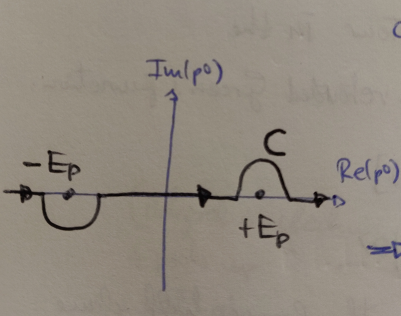
\includegraphics[width=0.3\linewidth]{gfx/Contour1}
	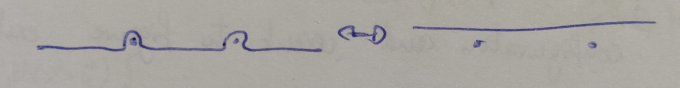
\includegraphics[width=0.7\linewidth]{gfx/Contour2}
	\caption{\itshape Integration contour for Feynman propagator of the real scalar field.}
	\label{fig:contour1}
\end{figure}
with $p^0$ integration along the real axis and with the limit $\epsilon \rightarrow 0$ after performing the integral.
The $i\epsilon$ term represents time ordering. Important is only the position of the poles with respect to the contour, thus the relative position.\\
\textbf{Note that \emph{this} is the place where off-shell contributions come into play since the integral in \ref{eq:feynmanpropagator} is over an unconstrained integration variable $\vec{p} = E_{\vec{p}}$.}

\begin{mybox}{Feynman propagator properties}
Note that the scalar Feynman propagator is symmetric in $x$ and $y$, i.e.
 \begin{equation}
 D_F(x-y) = D_F(y-x), \quad \mathrm{but}\; D(x-y) \neq D(y-x).
 \end{equation}
This will still hold true for interacting vacuum propagators. \textbf{Time ordering maps products of operators onto commuting numbers!} Because of this, expectation values of time ordered operators can
be expressed as path integrals as we will see later.
\end{mybox}
Use
\begin{align*}
	\frac{1}{p^2-m^2+i\epsilon} &= \frac{1}{p^2_0 - \vec{p}^2-m^2 + i\epsilon}=\frac{1}{p^2_0 - (E_p - i\epsilon)^2}\\
	Using \; &\left[-(E_p-i\epsilon)^2 = -E^2_p+2i E_p \epsilon = E^2_p + i \epsilon\right]\; \text{such that we further have} \\
	&= \frac{1}{p_0 - (E_p - \epsilon)} \frac{1}{p_0 +(E_p-i\epsilon)} \\
	\text{two poles at }\quad p_0=E_p -i\epsilon,\quad p_0 =-E_p + i \epsilon
\end{align*}
such that the integration reads as the following along the two possible contours \todo{Insert Feynman contour picture 2}
\begin{align*}
	D_F(x) &= \int \pmeasure \int_{\-\infty}^\infty \frac{\md p^0}{2 \pi} e^{-i p_0 x_0 + i \vec{p}\vec{x}} \frac{i}{p^0-(E_p-i \epsilon)} \frac{1}{p^0 + (E_p - i \epsilon)}\\
	D_F(x) |_{x^0>0} &= \int \pmeasure \underbrace{\frac{(-2 \pi i)}{2 \pi}}_{- \Leftarrow clockwise} \frac{i}{E_p +E_p} e^{-i E_p x^0+ i \vec{p}\vec{x}} = D(x)
\end{align*}
where the description here is equivalent to the Feynman contour with $p^0=-E_p$ and $p^0=E_p$. Therefore, the Feynman propagator is just a Green's function.
\subsubsection{Propagators as Green's functions}
\begin{mybox}{}
	The propagators are Green's functions for the KG equation
	\begin{align*}
		\mathcal{D}(\partial) G(x) &= i \delta(x) \\
		\mathcal{D}(\partial) &= (\partial^2 +m^2) \quad \Rightarrow \quad G(p) = \frac{i}{p^2-m^2},\; i.e.\\
		\mathcal{D}(\partial) D_A(x) &= \mathcal{D}(\partial) D_F(x) = \mathcal{D}(\partial) D_R(x) = -i  \delta(x).
	\end{align*}
Note that the scalar propagator is not a Green's function of the KG but satisfies
\begin{equation*}
	(\partial^2 + m^2) D(x) = 0.
\end{equation*}
\end{mybox}
The Feynman propagator $D_F(x-y)$ is a Green's function for the Klein-Gordon equation:
\begin{equation}
	(\partial^2_x + m^2) D_F(x-y) = -i \delta^{(4)}_D(x-y).
\end{equation}
The Green's function inverts the Klein-Gordon operator.
\begin{enumerate}
		\item
		\begin{figure}[h]
			\centering
			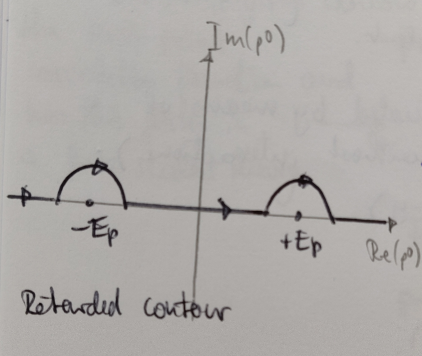
\includegraphics[width=0.7\linewidth]{gfx/Retardedcontour}
			\caption{\itshape Retarded contour.}
			\label{fig:retardedcontour}
		\end{figure} 
	 By avoiding both poles along a contour in the upper half-plane, the solution is the retarded Green's function
		\begin{equation}
			D_R(x-y)=\theta(x^0-y^0) [D(x-y)-D(y-x)]\equiv \theta(x^0-y^0) \expval{[\phi(x),\phi(y)]}{0}.
		\end{equation}
$D_R$ is useful in classical field theory if we know the initial value of some field configuration and want to figure out what it evolves into in the presence of the source.
It propagates information backward in time.
\item 
\begin{figure}[h]
	\centering
	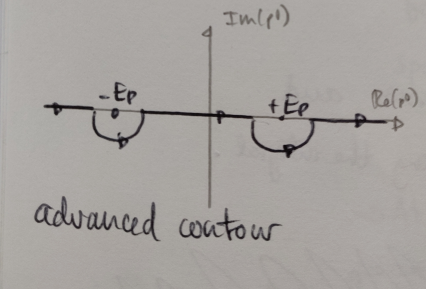
\includegraphics[width=0.7\linewidth]{gfx/Advancedcontour}
	\caption{\itshape Advanced contour.}
	\label{fig:advancedcontour}
\end{figure}
Avoiding both poles $p^0 = \pm \sqrt{E^2_{\vec{p}}}$ in the lower half plane yields the advanced Green's function
\begin{equation}
	D_A (x-y) = \theta(y^0-x^0) [D(x-y)-D(y-x)].
\end{equation}
$D_A$ is useful if we know the end point of a field configuration and want to figure out were it came from. It propagates forward in time.
\item $D_F(x-y)$ propagates positive frequency modes $e^{- i px}$ forward in time and negative frequency modes $e^{ipx}$ backward in time.
\end{enumerate}
Again, the ambiguity of Green’s functions results from an ambiguity in choice of contour when Fourier
transforming $G(p)$. One can write
\begin{equation}
	p^2 -m^2 = (p^0)^2 - E^2_p, \; i.e.\; G(p) = \frac{i}{p^2-m^2}=\frac{i}{(p^0)^2 - \abs{\vec{p}}^2 -m^2} = \frac{i}{(p^0-E_p)(p^0+E_p)}
	\end{equation}
and chose the contour - integrating counterclockwise - pushing both poles in the upper (advanced)
or lower (retarded) half of the complex plane, or pushing $p^0 = E_p$ down and $p^0 = −E_p$ up (Feynman) by
\begin{equation}
G(p) = \lim_{\tilde{\epsilon} \rightarrow 0} \frac{i}{(p^0-(E_p-i \tilde{\epsilon})) (p^0+E_p - i \tilde{\epsilon})}.
\end{equation}
Taking $\epsilon = - i \tilde{\epsilon}^2 + 2 \tilde{\epsilon}E_p$, dropping the quadratic term and ruthlessly switching integration and
limit then gives \ref{eq:feynmanpropagator} with a contour integral. But the contribution away from the real axis vanishes
if we send the contour radius to $\infty$ and close the contour in the lower or upper half appropriately
to the sign of $(x^0 − y^0 )$ because then the integrand falls off
\begin{equation}
\frac{e^{-ip(x-y)}}{p^2-m^2} \stackrel{Im(p^0)\rightarrow \infty}{\longrightarrow}0 \mathrm{\; at\;least\; as\;} e^{-Im(p^0)}.
\end{equation}
The fourth choice in contour, the Keldysh-propagator corresponding to anti-timeordering
\begin{equation}
	\label{eq:keldyshpropagator}
	D_K(x-y) =\theta(y^0-x^0) D(x-y) + \theta(x^0-y^0) D(y-x) = \bra{0}\bar{ \mathcal{T}} \phi(x) \phi(y) \ket{0}
\end{equation}
has no application here and is in fact algebraically dependent on the other three due to the identity
$θ(x^0 − y^0 ) + θ(y^0 − x^0 ) = 1$.

\subsubsection{Causality}
For causality to hold we need to measurements at spacelike distance not ot affect each other. This is guaranteed if any two local observables $O_1(x)$ and $O_2(y)$ at spacelike separation commute, i.e. 
\marginpar{local $\equiv$ local operators only depend on a local neighbourhood of the spacetime point $x$.}
\begin{equation}
\left[O_1(x),O_2(y)\right] \stackrel{!}{=} 0, \quad \mathrm{for} \quad (x-y)^2 < 0,
\end{equation}
even though $D_F (x − y) \neq 0$ for $(x − y)^2 < 0$. More specifically
\begin{equation}
\bra{0} \Delta(x-y) \ket{0} = D(x-y) - D(y-x) =0 \quad for \quad (x-y)^2 <0.
\end{equation}
This ensure that a measurement at $x$ cannot affect a measurement at $y$ when $x$ and $y$ are \emph{not causally connected}.\\
This theory is \emph{indeed causal} with commutators vanishing outside the lightcone 
\begin{align}
	\Delta(x-y)|_{(x-y)^2<0} &= [\phi(x),\phi(y)] |_{(x-y)^2<0} \\
	&= \int \pmeasure \frac{1}{2 E_p} \left[e^{-ip(x-y)} - e^{+i p(x-y)} \right]|_{(x-y)^2<0}=0 \nonumber
\end{align}
\marginpar{The states of QFT are non-local objects.}
because one can always make a Lorentz transformation such that $(x^0-y^0)=0$ for spacelike separation and change the minus sign of the integration variable.
This property will continue to hold in interacting theories, it is usually given as an axiom of local QFTs.\\
Note that the Fourier transformation of the commutator as indicator of free spectrum is
\begin{equation}
\Delta(k) = \frac{\pi}{E_k} \left[\delta(k^0-E_k)- \delta(k^0+E_k)\right]\left[\theta(k^0) - \theta(-k^0)\right].
\end{equation}
The fact that $[\phi(x),\phi(y)]$ is a $\mathbb{C}$-number function, rather than an operator, is a property of \emph{free fields only}.
\subsubsection{Vacuum spectral function and statistical propagator}
\begin{mybox}{}
	With the separation
	\begin{equation*}
		\bra{0}\mathcal{T}\phi (x) \phi(y)  \ket{0} = \half \bra{0} \{\phi(x),\phi(y) \} \ket{0} + \half sgn(x^0-y^0) \bra{0} [\phi(x),\phi(y)] \ket{0}
	\end{equation*}
we can define the spectral function $\rho$ as
\begin{equation}
\label{eq:spectralfunction}
\rho(x-y) :=i \bra{0} [\phi(x),\phi(y)] \ket{0} = i \bra{0} \Delta(x-y) \ket{0},
\end{equation}
and the statistical propagator $F$ as
\begin{equation}
	\label{eq:statisicalpropagator}
	F(x-y):= \half \bra{0} \{\phi(x),\phi(y) \} \ket{0},
\end{equation}
such that
\begin{equation}
	D_F(x-y) = F(x-y) - i\half sgn(x^0-y^0) \rho(x-y).
\end{equation}
\end{mybox}
Note that neither the statistical propagator nor the spectral function is a Green’s function, but
just sums of $D(x)$ such that
\begin{equation*}
	(\square +m^2) \rho (x) = (\square +m^2 ) F(x) = 0.
\end{equation*}
The Fourier transforms of $F$ and $\rho$ can be shown to be proportional to each other
\begin{equation}
	F (p) = ( \half + \delta(p^0)) \rho(p) .
\end{equation}

We will proof this as the special case of zero temperature of the KMS condition much later in the
context of thermal field theory, where it will become clear that $F$ keeps track of the occupation
of states, while $\rho$ keeps track what states exist (i.e. of the spectrum). In vacuum theory, $F$ is
uninteresting because of the above proportionality.


\subsubsection{How to perform the contour integral}
Define a function $g(z)$ with poles $z_0$ and apply Residue theorem:
\begin{equation*}
	g(z) =\frac{1}{E_p+z} e^{-i z (x^0-y^0)}, \quad z_0 =E_p, z=p^0.
\end{equation*}
\begin{align*}
	\Rightarrow \theta(x^0-y^0)&=g(z_0)=\theta(x^0-y^0) \left[\frac{1}{2 \pi i} \oint_{C_1} \frac{g(z) \md z}{z-z_0}\right]\\
	&=\theta(x^0-y^0) \left[\frac{1}{2 \pi i}\oint_{C_1} \left(\frac{1}{E_p+p^0} e^{-i p^0 (x^0-y^0)} \right) \frac{\md p^0}{p^0-E_p}\right] \\
	&= \theta(x^0-y^0) \left[\frac{1}{2 \pi i} \oint_{C_1} \md p^0 \frac{e^{-i p^0(x^0-y^0)}}{(p^0+E_p)(p^0-E_p)}\right] \\
	&=-\theta(x^0-y^0) \frac{1}{2 \pi i} \oint_C \md p^0 \quad \frac{e^{-ip^0(c^0-y^0)}}{(p^0 + E_p)(p^0-E_p)},
\end{align*}
where the minus comes about since the integral is performed clockwise ($\Rightarrow \times (-1)$) and because it picks up the pole at $+E_p \Rightarrow (-1) \times (+1)=-1$.\\
\begin{align*}
	\theta(y^0-x^0) \frac{1}{2 E_p} e^{i E_p (x^0-y^0)} &= \theta(y^0-x^0) g(z_0) \\
	&=\theta(y^0-x^0) \left[\frac{1}{2 \pi i} \oint_{C_2} \left(\frac{1}{p^0+E_p} e^{-i p^0 (x^0-y^0)} \right) \frac{\md p^0}{p^0-E_p}\right] \\
	&= - \theta(y^0-x^0) \frac{1}{2 \pi i} \oint_{C_2} \md p^0 \quad \frac{e^{-i p^0(x^0-y^0)}}{(p^0+E_p)(p^0-E_p)},
\end{align*}
where the minus sign comes about since the integral is performed counter-clockwise ($\Rightarrow \times +1$) and because it picks up pole at $-E_p \Rightarrow +1 \times (-1)=-1$. Thus, the Feynman propagator is given by the addition of both contours
\begin{align*}
	D_F(x-y) &= \int \pmeasure e^{i \vec{p}(\vec{x}-\vec{y})} \left[-\theta(x^0-y^0) \frac{1}{2 \pi i} \oint_{C_1} \md p^0 \frac{e^{-i p^0(x^0-y^0)}}{(p^0+E_p)(p^0-E_p)} \right.\\
	&\left. \qquad - \theta(y^0-x^0) \frac{1}{2 \pi i} \oint_{C_2} \md p^0 \frac{e^{-i p^0(x^0-y^0)}}{(p^0-E_p)(p^0+E_p)}\right]\\
		&\stackrel{R\rightarrow\infty}{=} - \oint \frac{\md^4 p}{(2 \pi)^4} \frac{1}{i} e^{-i p\cdot (x-y)} \underbrace{\left[\theta(x^0-y^0)+\theta(y^0-^0)\right]}_{=1} \frac{1}{(p^0+E_p)(p^0-E_p)} \\
		&= \oint \frac{\md^4 p}{(2 \pi)^4} \underbrace{\frac{i e^{-i p\cdot(x-y)} }{(p^0+E_p)(p^0-E_p)}}_{=p^2-m^2}.
\end{align*}




\newpage





\section{Interacting scalar theory}
\subsection{Introduction}
Our consideration of free scalar field theories showed, that the theory is \emph{exactly solvable}, we can determine the spectrum (Hilbert space is the Fock space of multi-particle states created from the vacuum $\ket{0}$) and the fields have particle excitations which do not interact. Free theories defined an EOM which is linear $(\partial^2+m^2) \phi=0$, which is exactly solved by Fourier analysis (i.e. different modes decouple). It is not possible to solve interacting theory in a closed form, but it is possible by perturbing around the free Lagrangian order by order in interactions, i.e. order by order in loop contributions.\\
\\
Interactions are described in QFT by potentials $V(\phi)$ beyond quadratic order
\begin{equation}
	V(\phi) = \underbrace{\half m^2_0 \phi^2}_{V_0 (\phi)} \qquad + \sum_{n\geq 3} \frac{\lambda_n}{n!} \phi^n.
\end{equation}
The coefficients $\lambda_n$ are called \emph{coupling constants}. Here we restrict ourselves to
\begin{equation}
V(\phi) = \half m^2_0 \phi^2 +\underbrace{\frac{1}{3!} g \phi^3+\frac{1}{4!} \lambda \phi^4}_{V_{\mathrm{int}}},\quad [\lambda_n]=4-n \neq 0 !,
\end{equation}
with the decomposition 
\begin{equation}
	\mathcal{L}=\mathcal{L}_0 +\mathcal{L}_{\mathrm{int}},\quad \mL_{\mathrm{int}}=-V_{\mathrm{int}}, \quad  \mL_{\mathrm{int}}=-\mathcal{H}_{\mathrm{int}},\; H=H_0 +H_{\mathrm{int}}.
\end{equation}
This linear decomposition comes about since we can always separate a theory into a background/free and an interacting solution. Could have different form, but linear decomposition is due to physical requirements:
\begin{enumerate}
	\item Want a local theory, i.e. local interactions $\leftrightarrow$ causality, i.e. \begin{equation}
	\phi^n(x) \in \mL: \qquad \int \int \phi^n(x) \phi^m(y)
	\end{equation}
	would not be local.
	\item $\mL$ has to be a Lorentz scalar, such that we look for terms $\phi^n(x), (\partial \phi)^2, \cancel{\partial \phi \phi^*}$.
	 \item Has to respect internal symmetry of the system. Eg. require $U(1)$ symmetry, then we cannot have $\psi \psi$ terms in $\mL$.
	 \item Renormalizability
	 \begin{equation}
	 	\mL = \left[\half (\partial_\mu \phi) (\partial^\mu \phi) - \half m^2 \phi^2\right] - \frac{\lambda_3}{3!} \phi^3-\frac{\lambda_4}{4!} \phi^4 - \underbrace{\frac{\lambda_5}{5!} \phi^5}_{non-renormalizable, [\lambda_5] <0} + \dots
	 \end{equation}
	 Ignore $\lambda_{n\geq5}$ terms since these theories are not renormalizable in $d=4$. Can always treat non-renormalizable theories as effective theories up to a certain cut-off scale.
\end{enumerate}
Introducing interaction terms leads to changes in the theory:\\
\begin{enumerate}
	\item The Hilbert space is different from the free theory
	\begin{enumerate}
		\item $\ket{0}\leftrightarrow$ vacuum of $H_0:\quad H_0\ket{0} =E_0 \ket{0}$.\\
		  $\ket{\Omega}\leftrightarrow$ vacuum of $H:\quad H\ket{\Omega}=E_{\Omega} \ket{\Omega}$
		with $\ket{\Omega}\neq \ket{0}$ in general.
		\item The mass of the momentum eigenstates of $H$ does no longer equal the parameter $m_0$ that appear in $\mL_0$.
		\item Bound states (e.g. hydrogen) may exist in the spectrum.
		\end{enumerate}
\item The states interact.
\end{enumerate}
The coupling constants are characterized as follows:
\marginpar{Only doing weakly coupled field theories here, because they can be considered as small perturbation of free field theory.}
\begin{enumerate}
	\item $[\lambda_3=g]=1$: The dimensionless parameter is $\lambda_3/E$, $E$ being the energy scale of the process of interest. This means that $\lambda_3 \frac{\phi^3}{3!}$ is a small perturbation at high energies $E\gg \lambda_3$, but a a large perturbation at low energies $E\ll \lambda_3$. Terms that we add to the Lagrangian with this behaviour are called \emph{relevant} because they are most relevant at low energies.
	\item $[\lambda_4=\lambda]=0$: This term is small if $\lambda_4 \ll 1$. Such perturbations are called \emph{marginal}. If $\lambda_4 \ll1$ then perturbation theory is applicable.
	\item $[\lambda_n]<0$ for $n\geq 5$: The dimensionless parameter is $(\lambda_n E^{n-4})$, which is small at low-energies and large at high energies. Such perturbations are called \emph{irrelevant}.
	\item Of the infinite number of interaction terms that we could write down, only $g$,$\lambda$ are needed (for real scalar field, else some more), because the irrelevant couplings become small at low-energies, our field of interest.
\end{enumerate}

\marginpar{Exact solution of non-free QFT is often not possible.}
\begin{mybox}{Lagrangians of interacting scalar field theories}
	\begin{equation}
		\mL = \half (\partial \phi)^2 + V(\phi) \quad V(\phi) = \frac{1}{2 !} m^2_0 \phi^2+ \frac{g}{3!} \phi^3+\frac{\lambda}{4!} \phi^4 + \mO(\phi^5)
	\end{equation}
	$\phi^4$-theory
	\begin{equation}
		\label{eq:lagrangianphi4}
		\mL = \half \left(\partial_\mu \phi \partial^\mu \phi - m^2 \phi^2\right) + \frac{\lambda}{4!} \phi^4,
			\end{equation}
	$\phi^3$-theory
	\begin{equation}
		\label{eq:lagrangianphi3}
		\mL = \half \left(\partial_\mu \phi \partial^\mu - m^2 \phi^2\right) + \frac{g}{3!} \phi^3,
	\end{equation}
	Breit-Wigner theory
	\begin{equation}
		\label{eq:lagrangianBreitWigner}
		\mL = \half \left(\partial_\mu \varphi \partial^\mu \varphi - m^2_{\varphi,0} \varphi^2\right) + \half \left(\partial_\mu \Phi \partial^\mu \Phi-m^2_{\Phi,0} \Phi^2\right) - \frac{\lambda}{2!}\Phi \varphi^2.
	\end{equation}
\end{mybox}
There is a physical justification to ignore $\mO(\phi^5)$ contributions, as we will find out in chapter
4 on renormalization. (Spoiler: its because couplings of $\mO(\phi^5)$ terms are zero in the IR in $\md = 3+1$.)\\
\\
Note that since the potential of $\phi^3$ theory is unbound from below, one does not expect a stable
vacuum to exist (even though quantum effects could in principle change the classical discussion).
However it can be a physical theory in combination with other fields that lead to a stable vacuum
that is bound from below, e.g. $\phi^3+\phi^4$ .




\subsubsection{Two-scalar Lagrangians, examples}
\begin{enumerate}
	\item $\phi^4$ theory:
\begin{equation}
	\mL = \half (\partial_\mu \phi)^2 -\half m^2 \phi^2 - \frac{\lambda}{4!}\phi^4
\end{equation}
with EOM
\begin{equation}
	(\partial^2 + m^2) \phi = - \frac{\lambda}{3!} \phi^3,
\end{equation}
which cannot be solved by Fourier decomposition.\\
\item Scalar Yukawa theory:
\begin{equation}
	\mL = \underbrace{\half \left[(\partial \phi)^2 - m^2 \phi^2\right]}_{KG}+\underbrace{\left[(\partial_\mu \psi^*)(\partial^\mu \psi) - M^2 \psi^*\psi\right]}_{free\,charged\,scalar}  -g  \psi^* \psi \phi.
\end{equation}
\end{enumerate}
\todo{insert 3)	}
\subsubsection{To to study interacting QFTS}
Not exactly solvable in $n>2$ dimensions. There are two possible approaches
\begin{enumerate}
	\item numerical solution, eg lattice gauge theory
	\item Perturbation theory, our approach. It is an expansion around free theory limit and is valid for weak couplings, where small means that that the NLO loop correction scales smaller than LO, since higher orders of the coupling become smaller (lecturer said that strong couplings are defined as $\lambda \geq 1$).
\end{enumerate}






\subsection{Källén-Lehmann spectral representation}
\subsubsection{Hilbert space}
Here we take a look at the spectrum of an interacting real scalar field theory in a manner valid for all types of interactions and without relying on perturbation theory. This representation gives a \emph{general expression} for the time ordered two-point function of an interacting quantum field theory as a sum of free propagators.\\
In interacting theory $[H,\vec{P}]=0$ still holds due  to Lorentz invariance. Their mutual eigenstates $\ket{\lambda_p}$ with
\begin{equation}
	H\ket{\lambda_p}=E_p(\lambda) \ket{\lambda_p}, \quad \vec{P}\ket{\lambda_p} = \vec{p} \ket{\lambda_p}
\end{equation}
correspond via a Lorentz boost to the state at rest, called $\ket{\lambda_0}$.\\
\begin{figure}
	\centering
	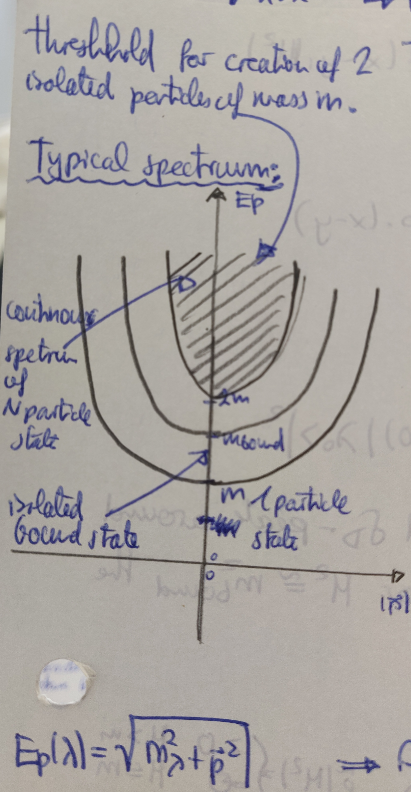
\includegraphics[width=0.7\linewidth]{gfx/Spectruminteractingtheory}
	\caption{\itshape Typical spectrum in the interacting theory.}
	\label{fig:spectruminteractingtheory}
\end{figure}
We can have the following types of $\ket{\lambda_{\vec{p}}}$:
\begin{enumerate}
	\item 1-particle states with $E^2_p = \vec{p}^2+m^2$, they have $p^{\nu}p_{\nu}=m^2$, $m\neq m_0$ (even in vacuum $m \neq m_0$ because of self-interactions).
	\item Bound states with no analogue in the free theory.
	\item 2-and $N$-particle states formed out of 1-particle and the bound states. In this case, we take $\vec{p}$ to the centre-of-mass momentum of the multi-particle state.
\end{enumerate}
\begin{mybox}{Hilbert space of interacting theory}
	Definition of interacting vacuum as Poincaréinvariant state
	\begin{equation}
	\label{eq:vacuumPoincareInvariant}
	U\ket{\Omega}= \ket{\Omega}\quad \forall U\in \mathcal{P}\; \Rightarrow \quad  H\ket{\Omega}=0.
	\end{equation}
	Interacting momentum eigenstates
	\begin{align}
	H\ket{\lambda_{\vec{p}}} &=E_{\vec{p}}(\lambda) \ket{\lambda_{\vec{p}}}\; \mathrm{with}\; E_{\vec{p}}(\lambda) :=\sqrt{\vec{p}^2+m^2_{\lambda}}\\
	\vec{P}\ket{\lambda_{\vec{p}}} &= \vec{p} \ket{\lambda_{\vec{p}}}
	\end{align}
where the single-particle state $\ket{1}_{\vec{p}}$ obeys
\begin{equation}
	P^mu \ket{1_{\vec{p}}}=p^\mu \ket{1_{\vec{p}}} \; with \; p^2=m^2
\end{equation}
with the interacting mass $m$. The interacting momentum eigenstates obey the \emph{completeness} relation
\begin{equation}
	\label{eq:completenessrelation}
	\mI=\ket{\Omega}\bra{\Omega}+ \sum_\lambda\hspace{-0.4cm}\int  \;\int \pmeasure \frac{1}{2 E_p(\lambda)} \ket{\lambda_p} \bra{\lambda_p},
\end{equation}
where $E_p(\lambda)=\sqrt{m^2_{\lambda}+\vec{p}^2}$ and $\sum$ includes a sum over 1-particle states, over all types of bound states as well as over all multiparticle states. $\int \md^3 p \dots$ refer to the centre-of-mass momentum of a state of species $\lambda$.\\
\end{mybox}
\begin{mybox}{Interacting equation of motion}
All these are created from the vacuum $\ket{\Omega}$. The crucial difference to the free theory is, that $ \phi(x)$ cannot simply be written as a superposition of its Fourier amplitudes $a(\vec{p})$ and $a^{\dagger}(\vec{p})$, because $\phi(x)$ \emph{does not obey the free e.o.m}, rather the interacting scalar operator equation of motion
\begin{equation}
	(\partial^2+m^2)\phi^H(x) = j^H(x),
\end{equation}
where generally $j$ is a function of $\phi$. The current can not create single particle states from the
vaccum, i.e.
\begin{equation}
\label{eq:interactingtheoryEOMcurrent}
	\bra{1_p} j(x) \ket{\Omega}=0.
\end{equation}
Thus, acting with  $\phi$ on $\ket{\Omega}$ \emph{does not} simply created a 1-particle state as in the free theory !
\end{mybox}
Proof of \ref{eq:interactingtheoryEOMcurrent}:
\begin{align*}
	\bra{1_p} j(x) \ket{\Omega} &= \bra{1_p} (\partial^2+m^2) \phi(x) \ket{\Omega}\\
	&=\bra{1_p} (\partial^2 +m^2) e^{-i Px} \phi(x) e^{-iPx} \ket{\Omega}\\
	&\stackrel{\ref{eq:vacuumPoincareInvariant}}{=} \bra{1_p}(\partial^2+m^2) e^{iPx} \phi(0) \ket{\Omega}\\
	&=\bra{1_p}(-P^2+m^2) e^{iPx} \phi(0) \ket{\Omega} \\
	&= \bra{1_p}(-p^2+m^2) e^{iPx} \phi(0) \ket{\Omega}\\
	&=\bra{1_p}(-p^2+m^2) \phi(x)\ket{\Omega}\\
	&=0.
\end{align*}
An aside (Reh-Schlieder property): local operators can not have an identically vanishing vacuum product, i.e.
\begin{equation}
	\label{eq:rehschlieder}
	\mO(x) \ket{\Omega} =0 \quad \Leftrightarrow \;\mO  =\hat{ 0}.
\end{equation}
\subsubsection{Propagator}
\begin{mybox}{Propagator interacting theory}
\begin{align}
	D(x-y)&:=\bra{\Omega}\phi(x)\phi(y)\ket{\Omega} \\
	&=\sum_\lambda \hspace{-0.4cm}\int \;\abs{\bra{\Omega}\phi(0)\ket{\lambda_0}}^2 \int \pmeasure \frac{1}{2 E_p} e^{-ip(x-y)}.\nonumber
\end{align}
\end{mybox}
\begin{mybox}{Feynman-propagator in interacting scalar theory}
We find the time-ordered interacting Feynman-propagator to be
\begin{align}
\expval{T\phi(x)\phi(y)}{\Omega} = \sum_{\lambda} \int& \frac{\md^4 p}{(2 \pi)^4} \frac{i}{p^2-m^2_{\lambda} +i\epsilon}\\
& e^{- i \cdot (x-y)} |\bra{\Omega}\phi(0)\ket{\lambda_0}|^2\nonumber,
\end{align}
or, equivalently, it turns out that in \emph{any} Lorentz-invariant theory we can
write the $2$-point function in the Kallén-Lehmann spectral representation as:
\begin{equation}
	\expval{T\phi(x)\phi(y)}{\Omega} = \int_0^{\infty} \frac{\md M^2}{2 \pi} \quad \rho(M^2) D_F(x-y,M^2),
\end{equation}
where we defined the Feynman propagator for a \emph{free} quantum field of mass $M$
\begin{equation}
	D_F(x-y, M^2) = \int \frac{\md^4 p}{(2 \pi)^4} \frac{i}{p^2-M^2+i\epsilon} e^{-i p\cdot (x-y)} 
\end{equation}
and the \emph{spectral function} (density)
\begin{equation}
	\rho(M^2) = \sum_{\lambda} 2 \pi \delta_D(M^2-m^2_{\lambda}) |\bra{\Omega} \phi(0) \ket{\lambda_0}|^2,
\end{equation}
which roughly speaking says "what are the masses of states that $\phi$ is creating
from the vacuum?”
\end{mybox}
In a free theory with mass $m^2$, the spectral density would read
\begin{equation*}
	\rho_{free}(M^2) = 2\pi \delta (m^2-M^2)
\end{equation*}
such that in the free theory the field $\phi$ just creates particles of mass $m$ as a Delta peak for $M^2=m^2$. For interacting theory however, we get a spectrum above the one-particle delta peak
\begin{equation*}
	\rho_{int}(M^2) = 2 \pi Z \delta (m^2-M^2) + stuff
\end{equation*}
note that the weight of the delta function has changed: as you now have some other probability to make
other things, the probability to create the single-particle state has been reduced.
We now have a non-vanishing probability to get higher than $1$-particle states via scattering, i.e. probability $p$ to create single particle $p\propto Z<1$, compare \ref{fig:spectruminteractingtheorymass}.\\
Note that whenever $Z$ is finite, it is at least true that we still create a particle. What if $Z$ drops to zero?
Then there is no probability that the φ field will create a physical particle. This is what happens in QCD
due to confinement.
\subsubsection{Self-energy}
\begin{mybox}{Self-energy and Dyson-Schwinger equation}
	The self energy  $−iM^2$ is the regular part of the RHS of the e.o.m. of the Feynman propagator
	\begin{equation}
		(\square_x+m^2)D_F(x,y)=:-i\delta(x-y) + i \int \md^4 z M^2(x,z)D_F(z,y)
	\end{equation}
	expressing the self-energy in terms of $j$ as defined by \ref{eq:interactingtheoryEOMcurrent} $(\square + m^2 ) \expval{\phi} = \expval{j}$
	\begin{equation}
	\label{eq:selfenergyCurrent}
		i \int \md^4z M^2(x, z)D_F (z, y) = \langle \mathcal{T} j(x)\phi(y)\rangle − \expval{j(x)} \expval{\phi(y)}
			\end{equation}
			allows for an operator evolution equation for the Feynman propagator that is closed in $\phi^{(H)}$, the
			Dyson-Schwinger equation (in compact integral notation)
			\begin{equation}
				\label{eq:dysonschwingereq}
				D_F = D^{(0)}_F + D^{(0)}_F (-i M^2) D_F.
			\end{equation}
\end{mybox}
Proof of \ref{eq:selfenergyCurrent}:\\
\begin{align*}
	&(\square_x+m^2)D_F(x,y) = (\square_x+m^2) \\
	&\times \left[\half \bra{0}\{\phi(x),\phi(y)\} \ket{0} + \half sgn(x^0-y^0) \bra{0}[\phi(x),\phi(y)]\ket{0} \right].
\end{align*}
The tricky term is now of course the $x^0$-derivative of the product sgn$(x^0-y^0)\rho(x,y)$
\begin{equation*}
	\partial^2_{x^0} sgn(x^0-y^0) \rho(x,y)=
\end{equation*}
with this we have
\begin{align*}
	(\square_x+m^2) D_F(x,y) &= -i \delta(x-y) + \half \expval{\{j(x),\phi(y)\}} \\
	&+ \half sgn(x^0-y^0) \expval{[j(x),\phi(y)]} - \expval{j(x)} \expval{\phi(y)}\\
	&=-i\delta(x-y) + \expval{\mathcal{T}j(x) \phi(y)} - \expval{j(x)} \expval{\phi(y)}
\end{align*}
i.e. we can express the self energy as
\begin{equation*}
	i \int \md^4 z M^2(x,z) D_F(z,y) = \expval{\mathcal{T} j(x) \phi(y)} - \expval{j(x)} \expval{\phi(y)}. \quad \blacksquare
\end{equation*}

\subsubsection{Wavefunction renormalization and spectrum of states via self energy}
\begin{mybox}{}
	We define
	\begin{equation}
		\label{eq:wavefunctionrenormalization}
		Z:= \abs{\bra{1_{\vec{0}} } \phi(0) \ket{\Omega}}^2
	\end{equation}
	and find that
	\begin{equation}
	\label{eq:statesWavefunctionRenorm}
	\bra{1_{\vec{p}} }\phi(x) \ket{\Omega} = \sqrt{Z} e^{ipx} |_{p_0 = E_{\vec{p}}},
	\end{equation}
	i.e. $Z$ is the probability for $\phi(x)$ to create a $1$-particle state from the interacting vacuum.\\
	$Z$ is a measure for the strength of the interaction with $0\leq Z\leq 1$ and
	\begin{equation}
		Z=1 \Leftrightarrow j(x) = \hat{ 0}\Leftrightarrow \rho(\mu^2) = \delta(\mu^2-m^2) \;\Leftrightarrow\; \mathrm{free\;theory}.
	\end{equation}
	$Z$ therefore takes as a rescale factor the effects of interactions or quantum fields into account,
	where $\ket{1_0}$ is the 1-particle state at rest.
\end{mybox}
In general we have
\begin{equation}
	\bra{\lambda\vp }\phi(x) \ket{\Omega} = \bra{\lambda_{\vec{0}}} \phi(0) \ket{\Omega} e^{ipx} |_{p_0 = E\vp(\lambda)}.
\end{equation}
Proof:\\
\begin{align*}
	\bra{\lambda\vp}\phi(x) \ket{\Omega} &= \bra{\lambda_{\vec{p}}}e^{iPx} \phi(0) e^{-iPx} \ket{\Omega}\\
	&= \bra{\lambda_{\vec{p}}} e^{iPx} \phi(0) \Omega \\
	&= \ket{\lambda_{\vec{p}}} \phi(0) \ket{\Omega} e^{ipx} |_{p_0 = E_p(\lambda)}\\
	&= \bra{\lambda_{\vec{p}}} U^{-1} \phi(0) U \ket{\Omega} e^{ipx} |_{p_0=E\vp(\lambda)}\\
	&= \bra{\lambda_{\vec{p}}} U^{-1} \phi(0) \ket{\Omega} e^{ipx} |_{p_0 =E\vp(\lambda)}\\
	&=\bra{\lambda\vz} \phi(0) \ket{\Omega} e^{ipx} |_{p_0 =E\vp(\lambda)}.
\end{align*}
For fields with spin, the wavefunction renormalization remains a Lorentz scalar, e.g.
\begin{align}
	Z_\phi &= \bra{1\vz}\phi(0) \ket{\Omega}\bra{\Omega}\phi(0) \ket{1\vz}\\
	Z_\psi &= \bra{1\vz}\bra{\psi}^A(0)\ket{\Omega} \bra{\Omega}\psi_A(0) \ket{1\vz}\\
	Z_A &= \bra{1\vz} A^\mu(0) \ket{\Omega}\bra{\Omega} A_\mu(0) \ket{1\vz}.
\end{align}
\begin{figure}[h!]
	\centering
	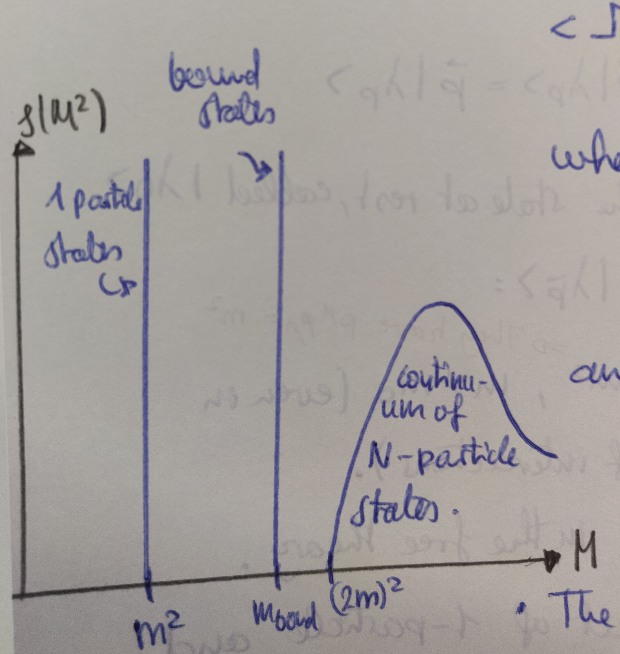
\includegraphics[width=0.7\linewidth]{gfx/SpectrumInteractingTheoryMass}
	\caption{\itshape Particle spectrum with respect to the mass.}
	\label{fig:spectruminteractingtheorymass}
\end{figure}
The 1-particle state lead to an isolated $\delta_D$-peak around $M^2=m^2$. Therefore, below $M^2\approx(2m)^2$ or $M^2\approx m^2_{\mathrm{bound}}$ the spetral function takes the form
\marginpar{In general $\int_0^{\infty} \frac{\md M^2}{2 \pi} \rho(M^2)=1$ holds.}
\begin{align}
	\rho(M^2) &= 2 \pi \delta_D(M^2-m^2) \quad Z \\
	&= 2 \pi \delta_D(M^2-m^2) Z+ \tilde{\rho}(M^2), \quad \tilde{\rho} (M^2) \left\{ \begin{array}{lr} \geq 0 & M>m \\
		=0 & M \leq m.
	\end{array}\right\}
\end{align}
with the \emph{wavefunction renormalization} $Z$ which takes as a rescale factor the effects of interactions or quantum fields into account
\begin{equation}
	Z=|\bra{\Omega}\phi(0)\ket{1_0}|^2,
\end{equation}
where $\ket{1_0}$ is the 1-particle state at rest.
\\
\\
We find the following statements 
\begin{enumerate}
	\item
	\marginpar{Calculation of the propagator yields the mass of the particle !}  The 1-particle state is the first analytic pole of the fully Feynman propagator at $m^2 \Rightarrow$ The mass-square $m^2$ of the particle is the location of the lowest-lying pole of the Fourier transformed propagator.
	\item Bound states appear at higher isolated poles
	\item N-particle states give rise to a branch cut beginning at $p^2=em^4$.
\end{enumerate}
The field strength renormalization in a free theory, i.e. $Z=1$, because $\phi(0)$ just creates the free particle from vacuum. In an interacting theory
\begin{equation}
	1 > \sqrt{Z} = \quad |\bra{\Omega} \phi(0) \ket{1_0}|,
\end{equation}
because $\phi$ creates not only 1-particle states and thus the overlap with the 1-particle states is smaller. Thus,
\begin{statements}
	$Z=1$ if and only if the theory is free.
\end{statements}
\begin{mybox}{Källen-Lehman spectral representation and mass gaps}
	\begin{align}
		&\int \md^4 x \bra{\Omega}\mathcal{T} \phi(x) \phi(y) \ket{\Omega} e^{ip(x-y)} \\
		&= \int_0^\infty \md \mu^2 \rho( \mu^2) \frac{i}{p^2-\mu^2+i\epsilon}\nonumber \\
		\mathrm{with}\; &\;\rho(\mu^2) := \sum_\lambda \hspace{-0.4cm}\int \; \abs{\bra{\Omega} \phi(0) \ket{\lambda_{\vec{0}}}}^2\delta(\mu^2-m^2_\lambda)
	\end{align}
where the spectral function is normalized
\begin{equation}
	\int \md \mu^2 \rho(\mu^2) =1.
\end{equation}
A theory is said to have a \emph{mass gap} if there exists and $ M^2>0$ such that (compare \ref{fig:spectruminteractingtheorymass})
\begin{equation}
\label{eq:massgap}
\rho(\mu^2) = Z \delta(\mu^2-m^2) + \rho_c(\mu^2) \;\; \mathrm{with}\; \rho_c=0 \;\mathrm{for} \; \mu^2 < M^2.
\end{equation}
A typical size for such an $M$ is the two particle bound state mass $M\approx 2m$. Another way of phrasing this in terms of the spectrum of the Hamiltonian
\begin{equation}
	H \ket{\psi} = E_\lambda \ket{\psi}\; \mathrm{with}\; E_\lambda \in \{0,[M,\infty) \} \quad \mathrm{with}\; M>0.
\end{equation}
If a theory possesses a mass gap, we can \emph{define the interacting mass} $m$ in terms of Källen-Lehmann spectral representation as the pole mass of the spectral function
\begin{align}
	\label{eq:polemassKLrep}
	\int \md^4x\bra{\Omega}\mathcal{T}\phi(x) \phi(y) \ket{\Omega}e^{ip(x-y)} &\stackrel{!}{=} \frac{iZ}{p^2-m^2+i \epsilon} \\
	&+ \int_{M^2}^\infty \md \mu^2\rho(\mu^2) \frac{i}{p^2-\mu^2+i\epsilon}.
\end{align}
\end{mybox}
Theories without a mass gap are generally believed to be unphysical, even though there is a lot of physical use for conformal theories which do not possess a mass gap.\\
\\
In the derivation of the interacting Feynman propagator we made use of the transformation behaviour of a scalar field under a Lorentz transformation
\begin{equation}
	x \mapsto x'=\Lambda x \quad \Rightarrow \quad U^{-1}(\Lambda)\phi(x') U(\Lambda) = \phi(x),
\end{equation}
because classically $\phi(x) \mapsto \phi'(x')=\phi(x)$ has its analogue in 
\begin{equation}
	\Leftrightarrow \bra{\alpha'} \phi(x') \ket{\beta'} = \bra{\alpha} \phi(x)\ket{\beta}=\bra{\alpha}U^{-1} \phi(x')U\ket{\beta}.
\end{equation}

\subsection{S-matrix and asymptotic in/out-states}
In interacting theory, the ladder operators in the mode expansion of the fields are now also time dependent, a simple canonical quantization via equal time commutation relations inducing time slices is not possible any more. This comes about since the interacting quantum field obeys an equation of motion 
\begin{equation}
	(\partial^2+m^2)\phi(x)=j(x)
\end{equation}
with source $j(x)$. On a technical note, these constructions have in practice to be done via wavepackets in order to guarantee bounded operators, i.e
 \begin{equation*}
 f_1(\vec{k}) \propto \exp\left[-\frac{(\vec{k}-\vec{k}_1)^2}{4 \sigma^2}\right] \quad \Rightarrow \; a^\dagger_1 \equiv \int \md^3 k f_1(\vec{k}) a^\dagger_{\vec{k}}.
 \end{equation*}
\subsubsection{In- and out Fock spaces and states}
\marginpar{Can be derived in the interaction picture as well, but here with in \& out states.}
Consider scattering of incoming states $\ket{\alpha,in}$ to outgoing states $\ket{\beta,out}$ with the aim of computing the QM transition amplitude, i.e. the probability amplitude for scattering of $\ket{\alpha,in}$ to $\ket{\beta,out}$.
\begin{mybox}{In and out states}
	Associated to the in and out states are the in and out field operators $\phi_{in}, \phi_{out}$, which satisfy
	\begin{equation}
		\partial^2+\underbrace{m^2}_{\neq m^2_0}  \phi_{in, out} (x) = 0 \quad \textcolor{red}{!}
	\end{equation}
	They have the same equal time commutation relations
	\begin{equation}
		[\phi_{in, out}(x),\Pi_{in,out} (y)]_{x^0=y^0} = i \delta^{(3)}_D (\vec{x}-\vec{y}),
	\end{equation}
	with others vanishing.
\end{mybox}
Associated to the in and out fields are two sets of creation and annihilation operators, $a^{\dagger}_{in}(\vec{p}), a_{in}(\vec{p}), a^{\dagger}_{out}(\vec{p}),a_{out}(\vec{p})$, acting in the same Hilbert space, on two complete sets (Fock spaces, initial $\mathcal{F}_{in}$ and final space $\mathcal{F}_{out}$). These operators satisfy the commutation relations
\begin{equation}
	[a_{in,out}(\vec{p}) , a^{\dagger}_{in,out} (\vec{p})]= i \delta_D(\vec{p}-\vec{p}'),
\end{equation}
with others vanishing.\\
The action of the creation operators on the respective vacua and states with a finite number of particles in the in and out states is given by
\begin{align}
	\ket{in, q_1, \dots,q_n} &=a^{\dagger}_{in}(\vec{q}_1) \dots a^{\dagger}_{in} (\vec{q}_n) \ket{\Omega,in}\\
	\ket{p_1,\dots, p_n, out} &= a^{\dagger}(\vec{p}_1) \dots a^{\dagger}(\vec{p}_n) \ket{\Omega,out}\\
	\mathcal{H}_i &= \mathrm{span}\{\ket{in, q_1,\dots, q_n}\}\\
	\mathcal{H}_f &= \mathrm{span}\{\ket{out,p_1,\dots,p_n}\},
\end{align}
where issues of normalization have been ignored!
\begin{mybox}{Relation between free vacuum $\ket{0}$ and interacting vacuum$\ket{\Omega}$}
		\begin{equation}
			\ket{0,in}=\ket{0,out} = \ket{\Omega}.
		\end{equation}
\end{mybox}
In the \emph{asymptotic past}, $t\rightarrow-\infty$, the in-states $\ket{i, in}$ are described as distinct wave packets corresponding to well-separated single particle states. Being far apart for $t\rightarrow-\infty$, they travel freely as individual states.\\
As these states approach each other, they start to interact and scatter into the final states. For $t\rightarrow\infty$ these final states are again asymptotically free and well-separated 1-particle states.
\begin{mybox}{}
	\begin{equation}
		\ket{\Omega;in} = \ket{\Omega;out} = \ket{\Omega}
	\end{equation}
	\begin{align}
		\phi_{in}(x) &= \int \pmeasure \frac{1}{\sqrt{2 E\vp}} \left(a_{in}(\vec{p}) e^{-ipx} +a^\dagger_{in}(\vec{p}) e^{ipx}\right) \\
		& \mathrm{with}\; E\vp=\sqrt{\vec{p}^2 +m^2},\; m\neq m_0\nonumber
	\end{align}
	with $\phi_{in}$ and $a_{in}$ obeying all the free commutation relations and therefore
	\begin{align}
		a^\dagger_{in}(\vec{p}) &= -\frac{i}{2 E\vp} \int \md^3 x e^{-ipx} \stackrel{\leftrightarrow}{\partial_0} \phi_{in}(x)\\
		\ket{p_i;in} &= \sqrt{2 E_{\vec{p}_i}} a^\dagger_{in} (\vec{p}_i)\ket{\Omega},
	\end{align}
and additionally the important relation
\begin{equation}
	\lim_{t\rightarrow-\infty} \bra{\alpha;out}\phi_{in}(x) \ket{\beta; in} = \frac{1}{\sqrt{Z}} \lim_{t\rightarrow-\infty} \bra{\alpha;out}\phi(x) \ket{\beta;in}
\end{equation}
that says that in the infinite past and future the theory behaves as if it was free. Relation \ref{eq:statesWavefunctionRenorm} can be expressed as
\begin{equation}
\bra{1\vp}\phi_{in}(x) \ket{\Omega} = \frac{1}{\sqrt{Z}} \bra{1\vp} \phi(x) \ket{\Omega} = e^{ipx}|_{p_0=E\vp}.
\end{equation}
All these relations are true also for the out-field with obvious replacements.
\end{mybox}
We can expand
\begin{equation}
	\phi_{in}(x) = \int \pmeasure \frac{1}{\sqrt{2 E_p}} \left[a_{in}(\vec{p}) e^{- i p\cdot x} +a^{\dagger}_{in} (\vec{p}) e^{i p\cdot x}\right].
\end{equation}
We can identify
\begin{equation}
	\lim_{t\rightarrow - \infty} \bra{\alpha}\phi\ket{\beta} = \lim_{t\rightarrow - \infty} \sqrt{Z} \bra{\alpha}\phi_{in} \ket{\beta} \; \Leftrightarrow\; \begin{array}{lr}
	\bra{\alpha}\phi \ket{\beta} \stackrel{t \rightarrow - \infty}{\rightarrow} \sqrt{Z} \bra{\alpha}\phi_{in} \ket{\beta} \\
	\bra{\alpha}\phi \ket{\beta} \stackrel{t\rightarrow +\infty}{\rightarrow} \sqrt{Z} \bra{\alpha} \phi_{out} \ket{\beta}
	\end{array}.
\end{equation}
\subsubsection{Examples for asymptotic states in scalar theory}
\begin{enumerate}
	\item \begin{equation}
		\mL =\mL_{KG} - U(x) \phi \quad \Leftrightarrow \quad (\partial^2 +m^2) \phi=- U(x),
	\end{equation}
	which describes scattering in an external potential. At $t=\pm\infty$, particles are far away from $U(x)$ if is falls off at $\infty\Rightarrow \ket{i},\ket{f}$ are eigenstates of $H_0$.
	\item \begin{equation}
		\mL = \mL_{KG} - \frac{\lambda}{4!} \phi^4 \quad \Leftrightarrow\quad (\partial^2+m^2) \phi= - \frac{\lambda}{3} \phi^3,
	\end{equation}
	which describes scattering in a \emph{dynamical potential}. Even at $t=\pm \infty$, can't turn off $H_{int}$, since the field is everywhere in space and time. However, even though a asymptotic they are never free states.
\end{enumerate}
In the end, problem is to calculate $\bra{f}S\ket{i}$ with $\ket{i,f}$ eigenstates of the free theory. 

\subsubsection{The S-matrix and the scattering process}
\begin{mybox}{The S-matrix}
	The S-matrix (scattering) maps the out-states onto the in-states (because the Fock spaces are isomorphic):
	\begin{equation}
		\ket{\alpha, in} = \quad S\ket{\alpha, out}, \;\Rightarrow S(\alpha,\beta):= \bra{\beta;out} S\ket{\alpha;out} = \bra{\beta;out}\ket{\alpha;in}
	\end{equation}
	with the properties
	\begin{enumerate}
		\item S is unitary $S^{\dagger} = S^{-1}$,
		\item $\phi_{in}(x) = \quad S \phi_{out}(x) S^{-1}$,
		\item $\ket{vac, in} =\ket{vac, out} = \ket{\Omega}$ and $S\ket{\Omega}=\ket{\Omega}$.
		\item $\phi_{in}(x) = S\phi_{out}(x) S^\dagger$
	\end{enumerate}
where the $\alpha$ and $\beta$ labels are usually chosen as momenta.
Thus, 
\begin{equation}
	S_{fi} = \lim_{t_{\pm} \rightarrow\pm \infty} \bra{f(t_+)} U(t_+,t_-) \ket{i(t_-)}_I \equiv \bra{f}S\ket{i},
\end{equation}
and
\begin{equation}
P(i\rightarrow f) =|\bra{f,in}S\ket{i,in}|^2 
\end{equation}
\emph{is the probability for scattering from initial states to the final states !}.\\
The vacuum is invariant $S\ket{\Omega}=\ket{\Omega}$.
\end{mybox}
Formally, the scattering process is described  by the following:\\
We have one Hilbert space for the whole scattering process from $t=-\infty$ to $t=+\infty$. There exist two Fock spaces $\mathcal{F}_{in}, \mathcal{F}_{out}$ in this Hilbert space, they are not disjoint because states can simply not participate in the scattering process. Long before the collisions, i.e. in the asymptotic past, we have well separated, free and independent wavepackets, the $\ket{\alpha,in}$ states with $\mathcal{F}_{in}=\mathrm{span}\{\ket{\alpha,in}\}$. Long after the collisions, we again have well separated, free and independent wavepackets, the $\ket{\beta,out}$ states with $\mathcal{F}_{out} = \mathrm{span}\{\ket{\beta,out}\}$. Then there exists an isomorphism between $\ket{\alpha,in}$ and $\ket{\beta,out}$, the $S$-matrix, with
\marginpar{$\mathcal{H}=\mathcal{F}_{out} \cup \mathcal{F}_{in}, \mathcal{F}_{out} \cap \mathcal{F}_{in} \neq \emptyset$.}
\begin{equation}
	\ket{\alpha, in}=S\ket{\alpha,out}, \qquad S:\mathcal{F}_{out} \rightarrow \mathcal{F}_{in}.
	\end{equation}
Then again, $\mathcal{F}_{in}=\mathrm{span}\{\ket{\alpha,in} = \phi_{in}(x)\ket{\Omega,in}\}$ and $\mathcal{F}_{out}=\mathrm{span}\{\ket{\beta,out}= \phi_{out}(x) \ket{\Omega,out}\}$ with $\ket{\Omega,in} = \ket{\Omega,out}=\ket{\Omega}$.\\
We thus find
\begin{align}
	S_{\beta \alpha} &:= \braket{\beta,out}{\alpha,in}, \qquad \ket{\alpha,in} = \sum_{\beta} S_{\beta \alpha} \ket{\beta,out}\\
	\Rightarrow \hat{S}\ket{\alpha,out} &=\sum_{\beta} S_{\beta \alpha} \ket{\beta,out} = \ket{\alpha,in} \\
	\Rightarrow S_{\beta \alpha} &= \braket{\beta,out}{\alpha,in} = \bra{\beta,out} \hat{S}\ket{\alpha,out}\\
	\bra{\beta,out}S^{\dagger} &= \bra{\beta,in} \qquad SS^{\dagger}=\sum_{\beta} \ket{\beta,in}\bra{\beta,in} = \mathcal{I}.
\end{align}
The probability amplitude for scattering from initial to final state.
\begin{mybox}{$T$-Matrix and Feynman amplitude $M$}
	$T$-matrix
	\begin{equation}
		\label{eq:tmatrix}
		\bra{f}S\ket{i} =: \delta_{fi} + T_{fi}.
	\end{equation}
	We will express the $\delta_{fi}$ more explicitly as the disconnected part of the $S$-matrix by LSZ reduction.\\
	Feynman amplitude $M$
	\begin{align}
		\bra{f}S\ket{i} &=: \delta_{fi} + i (2\pi)^4 \delta(p_f-p_i)M_{fi} \\
		i.e.\; T_{fi} &= i (2\pi)^4 \delta(p_f-p_i) M_{fi}.
	\end{align}
\end{mybox}
\begin{mybox}{optical theorem}
	Unitarity of the $S$ matrix immediately implies that
	\begin{equation}
	\label{eq:tmatrixunitarity}
		T^\dagger T = - i(T-T^\dagger)
	\end{equation}
	evaluating this equation in a free momentum eigenbasis by inserting a full set of states gives
	\begin{align}
		2 \mathrm{Im}M_{fi} &=\sum_{n=1}^\infty \left(\prod_{j=1}^{n} \int \frac{\md^3 q_j}{(2 \pi)^3} \frac{1}{2 E_{\vec{q}_j}} \right)\\
		&(2 \pi)^4  \delta(p_i -\sum_j q_j) M^*(f\rightarrow \{q_j\} ) M(i\rightarrow\{q_j\}) \nonumber
	\end{align}
which relates the imaginary part of an arbitrary scattering process to the product of two-scattering processes. One factor process goes from $i\rightarrow \{q_i\}$ and the other from $\{q_i\} \rightarrow f$ and they are contracted by a phase space integral over all possible intermediate states $\{q_i\}$.
\end{mybox}
This establishes \emph{cutting rules} for Feynman diagrams, which we will discuss under momentum Feynman rules.\\
In generic labels \ref{eq:tmatrixunitarity} implies for the diagonal elements of $T^\dagger T$
\begin{equation}
	\sum_\alpha \abs{T_{\alpha \beta}}^2 = 2 \mathrm{Im}T_{\beta  \beta}.
\end{equation}
This relates the \emph{total cross section} to the \emph{forward scattering amplitude}, because in a momentum basis $\mathrm{Im}T_{\beta\beta}\propto \mathrm{Im}M(k_i\rightarrow k_i)$ and $T^\dagger T\propto \sigma(k_i \rightarrow \mathrm{\;all\;possible\;final\;states})$.\\
\\
In S-matrix theory, the cluster decomposition principle states that if multi-particle processes $\alpha_1\rightarrow\beta_1,\dots,\alpha_N\rightarrow\beta_N$ are studied in $N$ very distant laboratories, then the S-matrix element for the overall process factorizes
\begin{equation*}
	S_{\beta_1+\dots + \beta_N,\alpha_1+\dots+\alpha_N}\rightarrow S_{\beta_1 \alpha_1} \dots S_{\beta_N \alpha_N} 
\end{equation*}
if for all $i\neq j$, all of the particles in states $\alpha_i$ and $\beta_i$ are at great spatial distance from all of the particles in states $\alpha_j$ and $\beta_j$.
\subsubsection{A note on the validity of the S-matrix}
At finite temperature, there’s no S-matrix because particles cannot get out to infinite distances from a collision without bumping into things. On the technical side of things, we can translate finite temperature requirement to the fact that the limes process \ref{eq:relationfreeInteractingvacuum} is not possible anymore, as it would imply going to zero temperature. Also, it seems quite possible that at very short
distances the description of events in four-dimensional flat space-time becomes inappropriate.





\subsection{The LSZ reduction formular}
\marginpar{As it is always the case for in and out states we regard the fully interacting theory, $\ket{\Omega}$.}
\begin{mybox}{The LSZ reduction formular}
The aim is to compute a S-matrix element $\braket{p_1,\dots,p_n,out}{q_1,\dots,q_r,in}$ for a real scalar field. Note that $p_1,\dots,p_n$ and $q_1,\dots,q_r$ are \emph{on-shell} since they correspond to the physical 4-momentum of the out-and incoming 1-particle states. We find

\begin{align}
&\bra{p_1,\dots,p_n;in}T\ket{q_1,\dots,q_r;in} = \\
&\prod_{k=1}^{n} \int \md^4 y_k e^{ip_k y_k} \prod_{l=1}^{r} \int \md^4 x_l e^{-iq_l x_l}\nonumber \\
&\cdot (\square_{y_1} +m^2) \dots (\square_{y_n} + m^2)(\square_{x_1} +m^2) \dots (\square_{x_n}+m^2)\nonumber \\
&\qquad  \bra{\Omega}\mathcal{T}\prod_{k=1}^n \phi(y_k) \prod_{l=1}^{r} \phi(x_l) \ket{\Omega}\nonumber
\end{align}
such that the Lemann-Symanzik-Zimmerman (LSZ) formula reads
\begin{align}
	\label{eq:lszformula}
	&\bra{p_1,\dots,p_n;in}T\ket{q_1,\dots,q_r;in} =\\
	& \left(\prod_{k=1}^{n} \frac{p^2_k-m^2}{i\sqrt{Z}} \right) \left(\prod_{l=1}^{r} \frac{q^2_l-m^2}{i\sqrt{Z}}\right)|_{p^2_k=q^2_l=m^2}\nonumber \\
	&\prod_{k=1 }^{n} \int\md^4 y_k e^{ip_k y_k} \prod_{l=1}^{r} \int \md^4 x_l e^{-i q_l x_l}\bra{\Omega} \mathcal{T}\prod_{k=1}^{n}\phi(y_k) \nonumber \\
	&\prod_{l=1}^{r} \phi(x_l) \ket{\Omega}|_{p^2_k=q^2_l=m^2}\nonumber
\end{align}
i.e. the connected S-matrix elements of $n$ to $m$ particles scattering are the coefficients of the multi-particle pole of the Fourier transformed $(n+m)$-point correlation function. The poles are where  the momenta are on-shell, i.e. the physical mass.
\end{mybox}
\marginpar{
	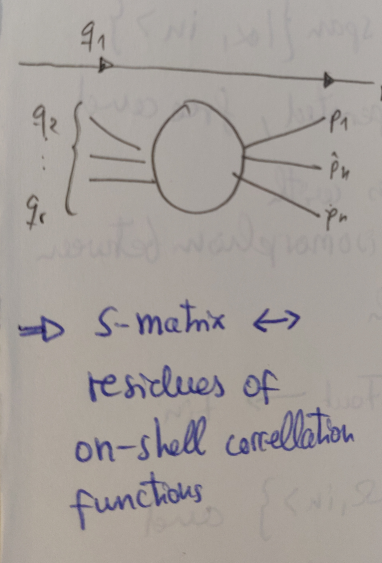
\includegraphics[width=0.3\marginparwidth]{gfx/disconnectediagram}
	\captionof{figure}{\itshape Disconnected diagram}
		\label{fig:disconnectediagram}
}
Because 
This LSZ-formula reduces the computation of the S-matrix to the computation of time-ordered correlation functions\\ $\expval{T\phi(y_1) \dots \phi(y_n) \phi(x_1)\dots \phi(x_n)}{\Omega}$ of the full interacting theory.\\
The first term describes a process where on of the in-and outgoing states are identical and do not participate in scattering.
Such an amplitude corresponds to a disconnected diagram, compare fig. \ref{fig:disconnectediagram}, and its computation reduces to computing an S-matrix element involving only $(r-1)$ in-and $(n-1)$ out-states.\\
For the connected term we find equivalently
\begin{align*}
	&\prod_{k=1}^{n} \int_{\mR^{3,1}} \md^4y_k e^{i p_k \cdot y_k} \prod_{l=1}^{r} \int_{\mR^{3,1}} \md^4x_l e^{-i q_l \cdot x_k}  \times \expval{T\prod_k \phi(y_k) \prod_l \phi(x_l)}{\Omega}\\
	&= \left(\prod_{k=1}^n \frac{i \sqrt{Z}}{p^2_k-m^2}\right) \left(\prod_{l=1}^{r} \frac{i \sqrt{Z}}{q^2_l - m^2}\right) \times \bra{p_1,\dots,p_n}S\ket{q_1,\dots,q_r}  |_{\mathrm{connected}}.
\end{align*}
which has poles as the momentum approaches the on-shell value $p^2 \rightarrow m^2$. Thus, if you want ot find $\braket{f}{i}$ compute $\expval{\phi\dots \phi}{0}$ and put all of the incoming momenta close to their physical/on-shell values. In that case, the correlation function should develop a pole. The resiude of this pole is the matrix element that you want. Note that the poles are the physical mass and not the bare mass.
\begin{statements}
	S-matrix $\leftrightarrow$ residues of on-shell correlation functions.
\end{statements}
$\expval{T\tilde{\phi}(p_1) \dots \tilde{\phi}(p_n) \tilde{\phi}(q_1)\dots \tilde{\phi}(q_r)}{\Omega} $ will in general be a sum of terms with different poles in the momenta. Only the term with the pole structure given precisely by $\prod_{k=1}^{n} \frac{1}{p^2_k - m^2} \prod_{l=1}^{r} \frac{1}{q^2_l-m^2}$ contributes to the connected S-matrix element.
\\
\\
Because of the appearance of $Z$ in \ref{eq:lszformula} it is useful to redefine our fields as
\begin{equation}
	\label{eq:renormalizedfield}
	\phi_r(x) := \frac{\phi(x)}{\sqrt{Z}}
\end{equation}
such that the \emph{renormalized field\ $\phi_r$} behaves like a free field near its S-matrix pole. Later we will introduce an additional term in the Lagrangian, that fixes the position of the pole such that the \emph{renormalized mass} of $\phi_r$ is given by the position of the pole.\\
	\\
	Incidentally this behaviour of S-matrix poles is true not only for fundamental fields (which by definition appear in the Lagrangian), but also for bound states which show up in the S-matrix as poles that are not at positions of fundamental masses.
	\todo{Derivation of LSZ formula, see gregor pp40}


\subsection{Bare mass scalar mass renormalization}
\begin{mybox}{}
	Definition of interacting mass as pole mass assuming a mass gap and continuous $M^2(p^2)$
	\begin{equation}
	D_F(p^2) = \frac{i}{p^2-m^2_0-M^2(p^2)} \stackrel{!}{=} \frac{iZ}{p^2-m^2} + (\mathrm{finite\;at}\;p^2=m^2)
	\end{equation}
	is a constraint to a complex function and has two real conditions
	\begin{align}
		M^2(m^2)&\stackrel{!}{=} m^2-m^2_0\\
		\mathrm{and}\; \frac{\md M^2}{\md p^2}(m^2) &\stackrel{!}{=} 1 - Z^{-1}.
	\end{align}
	In the presence of a discontinuity in $M^2$, i.e. non-vanishing Im$M^2$, the pole of the propagator is shifted away from the real axis and the renormalization condition has to be adjusted to
	\begin{align}
		D_F(p^2) &= \frac{i}{p^2-m^2_0-M^2(p^2)} \\
		&\stackrel{!}{=} \frac{iZ}{p^2-m^2-iZ\mathrm{Im}M^2(p^2)} \\
		&+ (\mathrm{finite\;at\;} p^2=m^2 + iZ\mathrm{Im}M^2(p^2))\\
		\Leftrightarrow\quad \mathrm{Re}M^2(m^2) &\stackrel{!}{=} m^2-m^2_0 \quad and ..?
	\end{align}
\end{mybox}
Anticipating confusion: Later on we will introduce perturbative renormalization (as opposed to bare perturbative renormalization here) and there the self energy is shifted $M^2\rightarrow M^2_r$ by computing with renormalized Feynman rules such that the renormalization conditions become especially simple, namely
\begin{align}
	D_F(p^2) \frac{i}{p^2-m^2-M^2_r(p^2)} \stackrel{!}{=}&\frac{i}{p^2-m^2} + (\mathrm{finite\;at\;} p^2=m^2) \\
	\Leftrightarrow\quad M^2_r(m^2) \stackrel{!}{=} & 0 \\
	\mathrm{and}\quad \frac{\md M^2_r}{\md p^2}(m^2) \stackrel{!}{=}&0.
\end{align}
Derivation of the two real conditions:\\
For two functions to agree in pole structure, they need to have the same pole positions and pole values (residues): The demand that the position $p^2=m^2$ of the pole of the RHS and LHS agree is equivalent ot
\begin{align*}
	\left[p^2-m^2_0 - M^2(p^2)\right]|_{p^2=m^2} &\stackrel{!}{=} (p^2-m^2) |_{p^2=m^2} = 0\\
	\Leftrightarrow\quad M^2(m^2) &=m^2-m^2_0.
\end{align*}
The demand that the residue agrees is equivalent to
\begin{equation*}
	\mathrm{Res}\left(D_F(p^2);m^2\right) \stackrel{!}{=} \mathrm{Res}\left(\frac{iZ}{p^2-m^2} ;m^2\right) = iZ.
\end{equation*}
To compute the Residue we expand the denominator
\begin{align*}
&	p^2-m^2_0 -M^2(p^2) = p^2-m^2_0 -M^2(m^2) \\
&+ \frac{\md M^2}{\md p^2}(m^2) (p^2-m^2) + \mO((p^2-m^2)^2)\\
	&=p^2-m^2- \frac{\md M^2}{\md p^2} (m^2) (p^2-m^2) +\mO((p^2-m^2)^2)\\
	&= (p^2-m^2) \left[1-\frac{\md M^2}{\md p^2} (m^2) + \mO(p^2-m^2)\right]\\
	&\Rightarrow\quad \mathrm{Res}(D_F(p^2);m^2) = \frac{i}{1-\frac{\md M^2}{\md p^2}(m^2)} \stackrel{!}{=} iZ \\
	&\Leftrightarrow\quad \frac{\md M^2}{\md p^2}(m^2) \stackrel{!}{=} 1-Z^{-1} \qquad \blacksquare.
\end{align*}

\subsection{Particle decay}
\begin{mybox}{Decay rates}
	\begin{align}
		&(2 \pi)^4 \delta(p-q) M(p\rightarrow q) =\\
		&\frac{p^2-m^2}{i \sqrt{Z}} \frac{q^2-m^2}{i \sqrt{Z}} \int \md^4 y e^{ipy} \int \md^4 x e^{-iqx}\\
		&\qquad \bra{\Omega}\mathcal{T}\phi(x) \phi(y) \ket{\Omega} |_{p^2=q^2=m^2}\nonumber \\
		&\Leftrightarrow\quad i M(p\rightarrow p) = \left(\frac{p^2-m^2}{i\sqrt{Z}}\right) D_F(p) \left(\frac{p^2-m^2}{i\sqrt{Z}}\right) |_{p^2=m^2} \\
		&=Z(-iM(p^2)) 
	\end{align}
	decay rate for $\Gamma \ll m^2$
	\begin{align}
	\Gamma_\Phi(p^2) &= -\frac{Z}{m} \mathrm{Im}M^2(p^2) \approx - \frac{Z}{m} \mathrm{Im}M^2(m^2)\\
	& = \frac{1}{m} \mathrm{Im}M(m\rightarrow m) =: \Gamma_\Phi\nonumber
	\end{align}
	decay rate in terms of scattering amplitudes via optical theorem
	\begin{align}
		\label{eq:decayrate}
		\Gamma_\Phi &= \frac{1}{2m} \sum_{n=1}^{\infty} \left(\prod_{j=1}^{n} \int \frac{\md^3 q_j}{(2 \pi)^3} \frac{1}{2 E_{\vec{q}_j}}\right) \\
		&(2\pi)^4 \delta(m-\sum_j q_j) \abs{M(m\rightarrow\{q_j\} )}^2.
	\end{align}
\end{mybox}
This is best discussed at the example of Breit-Wigner theory, with a heavy scalar $M\gg m$. There \todo{Breit Wigner theory decay}



\subsection{Perturbation theory around the free theory}
\subsubsection{Interaction (Dirac) picture}
One possible approach to perturbation theory is the interaction picture, in contrast to $S$-matrix calculations with asymptotic in-out states further down below.
\begin{mybox}{Interaction (Dirac) picture part I}
	Split $H=H_0+H_{int}$ with
	\begin{equation}
		H_0 = \int \md^3 x \half \left(\pi^2 + (\nabla \phi)^2+m^2_0 \phi^2\right)
	\end{equation}
	and operators
	\begin{align}
	\ket{\psi(t)}_I &= e^{iH_o0t} \ket{\psi(t)}_S,\quad \mO_I(t) = e^{iH_0t} \mO_S e^{-iH_0t}\\
	\phi^{(I)} (x) &:= e^{i H_0 (t-t_0)} \phi(t_0,\vec{x}) e^{-i H_0(t-t_0)} \\
	\pi^{(I)}(x) &:= e^{iH_0(t-t_0)} \pi(t_0,\vec{x}) e^{-i H_0(t-t_0)}.
	\end{align}
By construction, field operators in the interaction picture obey free time evolution
\begin{align}
	\label{eq:eomInteractionpicture}
	\partial^0 \phi^{(I)} (x) &= i \left[H_0,\phi^{(I)} (x)\right]\\
	(\partial^2+m^2_0) \phi^{(I)} (x) &=0
\end{align}
such that we can write them ito. creation operators
\begin{equation}
\phi^{(I)} (x) = \int \pmeasure \frac{1}{\sqrt{2 E\vp} }\left[a^{(I)}\vp e^{-ipx} + a^{(I)\dagger}\vp e^{ipx} \right].
\end{equation}
Hence, $\phi^{(I)}$ and $\pi^{(I)}$, and $a^{(I)\dagger}$ and $a^{(I)}$ are free fields, obeying all identities of free fields (thus also the commutation relations), especially
\begin{equation}
a^{(I)} (\vec{p}) \ket{0} = 0 \quad \forall \; \vec{p}.
\end{equation}
\end{mybox}
\begin{mybox}{Interaction (Dirac) picture part II}
Introducing the time evolution operator
\begin{equation}
	U(t,t_0) := e^{i H_0 (t-t_0)} e^{-i H(t-t_0)},
\end{equation}
which naturally appears in the relation \ref{eq:relationfreeInteractingvacuum} between the interacting and free vacuum (which is the reason why the interaction picture is useful in the first place), we find that
\begin{equation}
	\phi(x) = U^\dagger(t,t_0) \phi^{(I)} (x) U(t,t_0).
\end{equation}
This identity will be essential for constructing perturbation theory around the free theory. The time evolution operator satisfies the operator differential equation
\begin{equation}
	i\frac{\md}{\md t} U(t,t_0) = H^{(I)}_{int} (t) U(t,t_0)
\end{equation}
which we integrate to
\begin{align}
	\label{eq:dysonformula}
	U(t,t_0) &= - i \int_{t_0}^t H^{(I)}_{int} (t^\prime) U(t^\prime, t_0) \md t^\prime \nonumber\\
	&=\sum_{n=1}^{\infty} \frac{(-i)^n}{n!} \int_{t_0}^{t} \md t_1 \dots \int_{t_0}^t \md t_n \mathcal{T}\left(H^{(I)}_{int}(t_1)\dots H^{(I)}_{int}(t_n)\right)\nonumber\\
	&=:\mathcal{T} \exp\left(-i \int_{t0}^t H^{(I)}_{int} (t^\prime) \md t^\prime\right).
\end{align}
it is instructive to note that
\begin{equation}
H^{(I)}_{int}(t) = -\int \md^3 x \mL^{(I)}_{int}(t),
\end{equation}
such that the S-matrix can be written ito. the interacting Lagrangian in the interaction picture and as time evolution operator
\begin{equation}
	S= \mathcal{T} e^{-i \int \md^4x \mL^{(I)}_{int}} = \lim_{t\rightarrow\infty} U(t,-t).
\end{equation}
\end{mybox}
Useful properties of the time evolution operator are
\begin{align}
	UU^\dagger &= \mI \\
	U(t_1,t_2) &= U^{-1}(t_2,t_1) = U^\dagger(t_2,t_1)\\
	U(t_1,t_2)U(t_2,t_3) &= U(t_1,t_3) \quad for\, t_1 \geq t_2\geq t_3.
\end{align}
Note that the Dyson formula \ref{eq:dysonformula} can be seen as \emph{the} place where time ordering enters the operator description of vacuum QFT; "vacuum" because this formalism is only useful if we can do perturbation theory around the free theory, where it is possible to relate the free vacuum to the interacting vacuum as we will do in \ref{eq:relationfreeInteractingvacuum}.\\
\\
The first thing one has to do when describing thermal and non-equilibrium quantum field theory, is to generalize this notion of time ordering to imaginary time of $e^{-\beta H} = e^{-i (-i\beta) H}$ and the Schwinger-Keldysh path ordering respectively.\\
\\
This framework of the Dirac picture is sometimes used in old fashioned QM to treat explicit time dependency in the Hamiltonian by splitting $H=H_0 + V(t)$. Note that this is not the case in fundamental QFT, since an explicit time dependence necessarily breaks time translation invariance and indicates the negligence of an external system whose time evolution is unexplained. Instead, here the Dirac picture is used to relate an interacting theory to the free theory, which is exactly solvable, to then expand the appearing exponentials $\propto e^{-i \int \mL^{(I)}_{int}}$ in a (hopefully) small parameter. For the formalism it does not matter whether or not $H_{int}$ is time-dependent because either way we generally have
\begin{equation}
	[H_0,H] \neq 0 \; \Rightarrow \; H^{(I)}_{int} (t) = e^{i H_0 (t-t_0)} H_{int} e^{-i H_0(t-t_0)} \neq H_{int}
\end{equation}
such that $H^{(I)}_{int}(t)$ is \emph{time dependent}, i.e. perturbation theory around the free theory leads to a \emph{time dependent Hamiltonian formalism}.\\
\\
This idea of expansion around an exactly solvable theory is again applied in the Furry picture, where the expansion is done not around a free theory, but rather a classically interacting theory, which is still exactly solvable.\\
\\
Proof of \ref{eq:eomInteractionpicture}:
\begin{align*}
	\partial_0 \phi^{(I)} (x) &= i \left[H_0,\phi^{(I)} (x)\right] = e^{i H_0(t-t_0)} i [H_0,\phi(t_0,\vec{x})] e^{-i H_0(t-t_0)} \\
	&= e^{i H_0(t-t_0)} \pi(t_0,\vec{x}) e^{-i H_0 (t-t_0)} \\
	&= \pi^{(I)} (x).
\end{align*}
Such that, just as in free theory
\begin{align*}
	\partial^0 \partial_0 \phi^{(I)} (x) &= \partial^0 \pi^{(I)} (x) = e^{i H_0(t-t_0)} i [H_0,\pi(t_0,\vec{x})] e^{-iH_0(t-t_0)} \\
	&= (\nabla^2-m^2_0) \phi^{(I)} (x) \qquad \blacksquare.
\end{align*}

\subsubsection{Relating the interacting and free vacuum(Gell-Mann Low theorem) }
\begin{mybox}{}
	We introduce the "adiabatic limit" $\tau \rightarrow \infty (1-i\epsilon)$ which can be justified in the context of thermal field theory as the limit of zero temperature $T\rightarrow 0$ and find
	\begin{equation}
		\label{eq:relationfreeInteractingvacuum}
		\ket{\Omega;in} = \lim_{\tau\rightarrow \infty(1-i \epsilon)} \frac{U(t_0;-\tau) \ket{0}}{\bra{\Omega;in} U(t_0;-\tau) \ket{0}}
	\end{equation}
	and similarly for the out vacuum
	\begin{equation}
		\bra{\Omega;out} = \lim_{\tau\rightarrow \infty(1-i \epsilon)} \frac{\bra{0} U(\tau;t_0)}{\bra{0} U(\tau;t_0) \ket{\Omega;out}}.
	\end{equation}
\end{mybox}
Note that the awkward denominator drops out without worrying about normalization of $\ket{\Omega}$ assuming $\bra{\Omega}\ket{0}\neq 0$ if we compute objects like
\begin{equation}
	\frac{\bra{\Omega;out} \mO^{(H)} \ket{\Omega;in}}{\braket{\Omega;out}{\Omega;in}} = \lim_{\tau\rightarrow \infty(1-i \epsilon)} \frac{\bra{0}e^{iH\tau} \mO^{(H)} e^{-iH\tau} \ket{0}}{\braket{0}{0}}
		\end{equation}
		because it is also contained in 
		\begin{equation}
			\braket{\Omega}{\Omega} = \lim_{\tau\rightarrow \infty(1-i \epsilon)} \frac{\bra{0}U(\tau,-\tau) \ket{0}}{\abs{\bra{0}\ket{\Omega}}^2 e^{-i E_\Omega 2 \tau}}.
		\end{equation}
		Proof without reference to thermal field theory:\\
		Introduce the interpolation parameter $\epsilon$
		\begin{equation}
			H_\epsilon(\tau) = H_0 + e^{-\epsilon \abs{\tau}} H_{int} 
		\end{equation}
		which adiabatically, i.w. for $\tau\rightarrow \infty$, $\epsilon\rightarrow 0^+$, interpolates between free and interacting theory
		\begin{equation}
			\ket{\alpha;out} = \lim_{\tau\rightarrow \infty(1-i \epsilon)} e^{-i H\tau } \ket{\alpha}
		\end{equation}
		which can be understood as an alternative definition of an asymptotic out-state. Now we express $\ket{\alpha;out}$ in Hamiltonian eigenstates via insertion \ref{eq:completenessrelation}  
		\begin{equation*}
			\ket{\alpha;out} = \ket{\Omega}\braket{\Omega}{\alpha;out} + \sum_\lambda \hspace{-0.4cm}\int \; \int \pmeasure \frac{1}{2E\vp(\lambda)} \ket{\lambda\vp}\braket{\lambda\vp}{\alpha;out}
		\end{equation*}
	and note that in the adiabatic limit $\tau\rightarrow \infty (1-i\epsilon)$ all except the ground state contribution vanish
	\begin{equation*}
		\ket{\alpha;out} = \lim_{\tau\rightarrow \infty(1-i \epsilon)} e^{-iE_\Omega \tau} \ket{\Omega}\braket{\Omega}{\alpha}
	\end{equation*}
specifying the ground state $\ket{\alpha}=\ket{0}$ and solving for $\ket{\Omega}$ gives
\begin{equation*}
	\ket{\Omega} = \lim_{\tau\rightarrow \infty(1-i \epsilon)} \frac{e^{-i H\tau} \ket{0}}{e^{-i E_\Omega \tau} \braket{\Omega}{0}}
\end{equation*}
using $H_0\ket{0}=0 \Rightarrow e^{-iH_0 t} \ket{0}=\ket{0}$ and $U(t;t_0) = e^{iH(t-t_0)} e^{-i H_0(t-t_0)}$, this is the result \ref{eq:relationfreeInteractingvacuum}. $\blacksquare$

\subsubsection{Correlators in the interaction picture - Again-Maybe reduce this subsubsection away}
The computation of the full correlator shall now be reduced to a calculation in terms of free-field creation/annihilation operators and the free-field vacuum. This is achieved in the interaction picture: 
	\marginpar{$H=H_0+H_{int}$, $[H_0,H]\neq 0$.}
\begin{mybox}{Operator fields in the interaction picture}
	The time dependence of operators in governed by $H_0$, while the time dependence of states is governed by $H_int$:
	\begin{align}
		\phi_I(t,\vec{x}) &= e^{i H_0 (t-t_0)} \phi(\vec{x},t_0) e^{-i H_0 (t-t_0)} \\
		\Pi_I(t,\vec{x}) &= e^{i H_0 (t-t_0)} \Pi(\vec{x},t_0) e^{-i H_0 (t-t_0)} \\
		\ket{\psi(t)}_I &= e^{i H_0 t} \ket{\psi(t)}_S \\
		H_I &\equiv (H_{\mathrm{int}})_I = e^{i H_0 t} (H_{\mathrm{int}})_S e^{-i H_0 t}.
	\end{align}
	Then $\phi_I(t,\vec{x})$ satisfies the free Klein-Gordon equation
	\begin{equation}
	(\partial^2+m^2_0) \phi_I(t,\vec{x}) = 0,
	\end{equation}
	thus a \emph{free mode expansion} is possible.
\end{mybox}
The free mode expansion reads
\begin{equation}
\phi_I(x) = \int \pmeasure \frac{1}{\sqrt{2 E_p}} \left[a_I(\vec{p}) e^{-i p\cdot x} + a^{\dagger}_I(\vec{p}) e^{i p\cdot x} \right]
\end{equation}
with
\begin{equation}
[\phi_I(t,\vec{x}), \Pi_I(t,\vec{y})]=i \delta^{(3)}_D(\vec{x}-\vec{y}), \quad [a_I(\vec{p}),a^{\dagger}_I(\vec{q})] = (2 \pi)^3 \delta^{(3)}_D(\vec{p}-\vec{q}).
\end{equation}
Therefore the results of the free theory carry over:
\begin{equation}
H_= \ket{0}=0, \qquad a_I(\vec{p})\ket{0}=0.
\end{equation}
The transition to Heisenberg picture can now be done with
\begin{equation}
\phi(t,\vec{x}) = U^{\dagger}(t,t_0)  \phi_I(t,\vec{x}) U(t,t_0)
\end{equation}
with the time-evolution operator
\begin{equation}
U(t,t_0) = e^{i H_0(t-t_0)} e^{-i H(t-t_0)} = \hat{T}e^{-i \int_{t_0}^{t} H_I(t') \md t'}.
\end{equation}
\begin{mybox}{How to compute the correlators}
	The logic is now to replace the Heisenberg picture operators $\phi(x)$ om the correlator $\expval{T\phi(y_1) \dots \phi(y_n) \phi(x_1) \dots \phi(x_r)}{\Omega}$ by the interaction picture operators $\phi_I(x)$ because they obey a \emph{free mode expansion}.\\
\end{mybox}
We find \emph{Dyson's formula} for the time-evolution operator
\begin{align}
	U(t,t_0) &= \mathcal{I} + \sum_{n=1}^{\infty} \left(\frac{1}{i}\right)^n \int_{t_0}^{t} \md t_1 \int_{t_0}^{t_1} \md t_2 \dots \int_{t_0}^{t_{n-1}} \md t_n \underbrace{H_I(t_1)H_I(t_2)\dots H_I(t_n)}_{\mathrm{these \, are\, time-ordered}}\\
	&= \sum_{n=0}^{\infty} \frac{(-i)^n}{n!} \int_{t_0}^{t}\md t_1 \int_{t_0}^{t} \md t_2 \dots \int_{t_0}^{t} \md t_n T H_I (t_1)H_I(t_n) \\
	&=T e^{-i \int_{t_0}^{t} \md t'H_I(t')}.
\end{align}
With the properties
\begin{align}
	U^{\dagger}(t_1,t_2) &=U^{-1}(t_1,t_2) = U(t_2,t_1) \\
	U(t_1,t_2)U(t_2,t_3) &= U(t_1,t_3) \quad \mathrm{for} \quad t_1 \geq t_2 \geq t_3.
\end{align}
There is an equivalent representation of the time-evolution operator
\begin{align}
	U(t) &= \lim_{n\rightarrow \infty} \left\{  \left[1-i H_{I,int} (\tau_{n-1}) (\tau_n - \tau_{n-1})\right] \right. \\
	&\left.\left[1-i H_{I,int}(\tau_{n-2}) (\tau_{n-1}-\tau_{n-2}) \right]\dots \left[1-iH_{I, int} (\tau_0) (\tau_1-\tau_0) \right]   \right\}.
\end{align}
\\
\\
Furthermore we find a relation between the free vacuum $\ket{0}$ and the interacting vacuum $\ket{\Omega}$. The time-evolution of the free vacuum is
\begin{equation}
	e^{-iHT} \ket{0} = e^{-iHT} \sum_{\ket{n}} \ket{n} \braket{n}{0} = e^{- iE_{\Omega}T} \ket{\Omega}\braket{\Omega}{0}+\sum_{\ket{n} \neq \ket{\Omega}} e^{-iE_n T}\ket{n}\braket{n}{0}.
\end{equation}
The idea is, that the second term must vanish for $T\rightarrow \infty$, because excited states will go down eventually.\\
If $H_0 \ket{0}=0$, then $H\ket{\Omega} =E_{\Omega}\ket{\Omega}$ with $E_{\Omega}\neq 0$ and $E_n > E_{\Omega} \forall \ket{n} \neq \ket{\Omega}$. So if we formally take the limit $T\rightarrow\infty(1-i\epsilon)$, then $e^{-i E_n T}$ is stronger suppressed and only the vacuum $\ket{\Omega}$ survives:
\begin{align}
	\ket{\Omega} &= \lim_{T\rightarrow\infty(1-i\epsilon)} \left[e^{-i E_{\Omega} (t_0 - (-T)) \braket{\Omega}{0}}\right]^{-1} U(t_0,-T) \ket{0} \\
	\Rightarrow \expval{\hat{T}\phi(x) \phi(y)}{\Omega} &= \lim_{T\rightarrow \infty(1-i \epsilon)} \frac{\expval{\hat{T} \left(\phi_I(x) \phi_I(y) e^{-i \int_{-T}^{T} \md t H_I(t)} \right)}{0}}{\expval{\hat{T} e^{-i \int_{-T}^{T} \md t H_I(t)}}{0}}
\end{align}
with the same reasoning for higher n-point correlators.\\
Thus, gauge $E_0$ energy to be zero: $H_0 \ket{0}=E_0 \ket{0}=0$ such that $H\ket{\Omega} =E_{\Omega} \ket{\Omega} \neq 0$.
\begin{mybox}{Logic on how to compute correlators}
	Replace Heisenberg with interaction picture operators, from this we get $e^{-i \hbar \int H_I}$. Then go over from $\ket{\Omega}\rightarrow\ket{0}$ with given relation. Then compute $\expval{\phi \dots \phi}{0}$ explicitly via Wick normal ordering $\Rightarrow$ express results in terms of Feynman diagrams.
\end{mybox}

\subsubsection{$N$-point correlator computation in the interaction picture}
\begin{mybox}{}
	\begin{align}
		\label{eq:correlatorsMaster}
		& \frac{\bra{\Omega;out} \mathcal{T} \prod_{i=1}^{N} \phi(x_i) \ket{\Omega;in}}{\braket{\Omega;out}{\Omega;in}}=\\
		&\lim_{\tau\rightarrow \infty(1-i \epsilon)} \frac{\bra{0} \mathcal{T} \prod_{i=1}^{N} \phi^{(I)}(x_i) \exp \left(-i \int_{-\tau}^{\tau} H^{(I)}_{int}(t^\prime) \md t^\prime \right) \ket{0}}{\bra{0} \mathcal{T} \exp \left(-i \int_{-\tau}^{\tau} H^{(I)}_{int} (t^\prime) \md t^\prime \right) \ket{0}}\nonumber
	\end{align}
or, identifying the S-matrix
\begin{equation}
	\frac{\bra{\Omega;out} \mathcal{T}\prod_{i=1}^{N} \phi(x_i) \ket{\Omega;in}}{\braket{\Omega;out}{\Omega;in}} = \frac{\bra{0}\mathcal{T} \prod_{i=1}^{N} \phi^{(I)} (x_i) S\ket{0}}{\bra{0}S\ket{0}}.
\end{equation}
\end{mybox}
Note that in the language of correlators, the Feynman propagator is the $2$-point correlator and the vacuum expectation value is the $1$-point correlator.\\
\\
Note that this result and its derivation nicely display why computing time ordered correlation functions is natural in vacuum QFT: \\
correlations functions contain the same information regardless if we time order or not, but time ordering allows for manageable expression \ref{eq:correlatorsMaster}, in which we can pull $\mathcal{T}$ (which appears in the time evolution operator \ref{eq:dysonformula} either way) over the correlator fields $\phi(x_i)$ and do perturbation theory by expanding the exponential while never having to worry about the ordering of the field $\phi^{(I)}(x_i)$ and $\phi^{(I)}(t^\prime)$. Under the time ordering symbol we can freely commute them ignoring their operator nature! \\
A more natural language, where this feature of commuting fields is present right away is the pathintegral formalism. There the analogous result \todo{insert reference here gregor p47} displays the natural appearance of time ordering in vacuum QFT.\\
\\
Proof of \ref{eq:correlatorsMaster}:\\
we start by computing the $2$-point correlation function, assuming $x_0>y_0>t_0$, and worry about time ordering and higher order functions later.\\
Choosing $t_0$ such that $U^\dagger (x^0,t_0)\phi^{(I)}(x) U(x^0,t_0)= \phi(x)$ (and likewise for $\phi(y)$), and making use of our result \ref{eq:relationfreeInteractingvacuum} for the interacting vacuum we get
\begin{align*}
	& \bra{\Omega}\phi(x) \phi(y) \ket{\Omega} = \bra{\Omega}U^\dagger(x^0,t_0) \phi^{(I)}(x) U(x^0,t_0) U^\dagger(y^0,t_0) \phi^{(I)}(y) U(y^0,t_0)\ket{\Omega}\\
	&\stackrel{\ref{eq:relationfreeInteractingvacuum}}{=} \lim_{\tau\rightarrow \infty(1-i \epsilon)}
	\frac{\bra{0}U^\dagger(t_0;\tau) U^\dagger(x^0,t_0) \phi^{(I)}(x) U(x^0,t_0) U^\dagger(y^0,t_0) \phi^{(I)}(y) U(y^0,t_0) U(t_0;-\tau) \ket{0}}{\left(e^{-iE_\Omega (\tau-t_0)} \braket{0}{\Omega} \right) \left(e^{-i E_\Omega(t_0+\tau)} \braket{\Omega}{0} \right)} \\
	&= \lim_{\tau\rightarrow \infty(1-i \epsilon)}\frac{\bra{0} U(\tau,t_0) U(t_0,x^0) \phi^{(I)}(x) U(x^0,t_0) U(t_0,y^0) \phi^{(I)} (y) U(y^0,t_0) U(t_0;-\tau) \ket{0}}{\left(e^{-i E_\Omega (\tau-t_0)} \braket{0}{\Omega}\right)\left(e^{-iE_\Omega(t_0+\tau)} \braket{\Omega}{0}\right)} \\
	&= \lim_{\tau\rightarrow \infty(1-i \epsilon)}\frac{\bra{0} U(\tau,x^0) \phi^{(I)} (x) U(x^0,y^0) \phi^{(I)} (y) U(y^0,-\tau) \ket{0}}{\left(e^{-i E_\Omega (\tau-t_0)} \braket{0}{\Omega}\right) \left(e^{-i E_\Omega(t_0+\tau) } \braket{\Omega}{0}\right)}\\
	&= \lim_{\tau\rightarrow \infty(1-i \epsilon)}\frac{\bra{0}U(\tau,x^0) \phi^{(I)}(x) U(x^0,y^0) \phi^{(I)}(y) U(y^0,-\tau) \ket{0}}{\abs{\braket{\Omega}{0}}^2 e^{-iE_\Omega e\tau} }\\
	&=\lim_{\tau\rightarrow \infty(1-i \epsilon)} \frac{\bra{0}U(\tau,x^0) \phi^{(I)}(x) U(x^0,y^0) \phi^{(I)}(y) U(y^0,-\tau)\ket{0}}{\bra{0}U(-\tau,\tau) \ket{0}}.
\end{align*}
Now we use that we assumed $x_0>y_0>t_0$ such that we can write
\begin{equation*}
	U(\tau,x^0) \phi^{(I)}(x) U(x^0,y^0) \phi^{(I)}(y) U(y^0,-\tau) = \mathcal{T}\phi^{(I)}(x) \phi^{(I)} (y) U(\tau,x^0) U(x^0,y^0) U(y^0,-\tau)
\end{equation*}
i.e.
\begin{align*}
	& \bra{\Omega}\phi(x)\phi(y)\ket{\Omega} = \lim_{\tau\rightarrow \infty(1-i \epsilon)}\frac{\bra{0}U(\tau,x^0) \phi^{(I)}(x) U(x^0,y^0) \phi^{(I)}(y) U(y^0,-\tau) \ket{0}}{\bra{0}U(\tau,-\tau)\ket{0}}\\
	&= \lim_{\tau\rightarrow \infty(1-i \epsilon)} \frac{\bra{0}\mathcal{T}\phi^{(I)}(x) \phi^{(I)}(y) U(\tau,x^0) U(x^0,y^0) U(y^0,-\tau) \ket{0}}{\bra{0}U(\tau,-\tau)\ket{0}}\\
	&= \lim_{\tau\rightarrow \infty(1-i \epsilon)} \frac{\bra{0}\mathcal{T}\phi^{(I)}(x) \phi^{(I)}(y) U(\tau,-\tau) \ket{0}}{\bra{0}U(\tau,-\tau)\ket{0}}.
\end{align*}
Repeating this calculation for the other case $x_0<y_0<t_0$ and generalizing to $N$ fields (which is straightforward) gives the result \ref{eq:correlatorsMaster}$\blacksquare$.\\
\\
Most of the awkwardness about this derivation, the adiabatic limit $\tau\rightarrow \infty (1-i\epsilon)$ and the necessity of computing the denominator $\braket{\Omega;out}{\Omega;in}$, is absent if one start from non-equilibrium quantum field theory.\\
In non-equilibrium QFT one considers correlation functions
\begin{equation}
	\expval{\mO} := \tr \{\rho(t_0) \mO^{(I)}(x)\}
\end{equation}
where $\rho(t_0)$ contains all information about the initial state. This initial value problem is no longer translation invariant and one finds that it is necessary to integrate along the Keldysh contour. The reduction of this Keldysh nonequilibrium formalism to vacuum theory happens via three steps (compare for more details \ref{eq:reductionQFT}):
\begin{enumerate}
\item We make the choice for the density matrix $\rho_0$ which corresponds to thermal equilibrium, i.e.
\begin{equation}
	\rho(t_0) = \rho_\beta := \frac{e^{-\beta H}}{\tr e^{-\beta H}}.
\end{equation}
This restores translation invariance (since $\rho_\beta$ now commutes with $P^\mu$ again) such that $F(x,y) = F(x-y)$ and $\rho(x,y)=\rho(x-y)$, and gives rise to an identity in Fourier space: the dissipation fluctuation relation
\begin{equation}
	F^{(eq)}(p) = -i (\half + n_B(p^0)) \rho^{(eq)} (p).
\end{equation}
\item Taking $\beta \rightarrow\infty$, i.e. going to zero temperature reduces the equilibrium density matrix to a projection operator onto the vacuum (up to a multiplicity factor in case of degeneracy of the vacuum), i.e.
\begin{equation}
	\rho_\beta = \frac{e^{-\beta H}}{\tr e^{-\beta H}} \stackrel{\beta \rightarrow\infty}{\longrightarrow} \ket{\Omega}\bra{\Omega}.
\end{equation}
\item Lastly, the construction of asymptotic in-and out states allows us to only use objects on the forwards part of the contour $\mathcal{C}^+$, i.e. $G^{++}=D_F$ which is the Feynman propagator: The Keldysh contour emerges from
\begin{align*}
	\tr \rho(x^0) \mO(\vec{x}) &= \tr U(x^0,t_0)\rho(t_0) U(t_0,x^0) \mO(\vec{x})\\
	&= \tr \rho(t_0) U(t_0,x^0) \mO (\vec{x}) U(x^0,t_0) \\
	&= \tr \rho(t_0) U(t_0,x^0) \mO(\vec{x}) U(x^0,\infty) U(\infty,t_0).
\end{align*}
If we are only interested in vacuum expectation values we take
\begin{subequations}
\begin{align}
	&\tr \rho_\beta \mO^{(H)}(x) \stackrel{\beta \rightarrow\infty}{\longrightarrow} \bra{\Omega}\mO(x) \ket{\Omega}\nonumber\\
	=& \bra{\Omega} U(t_0,x^0) \mO^{(I)}(x) U(x^0,t_0) \ket{\Omega}\nonumber \\
	=& \bra{\Omega} U(t_0,x^0) \mO^{(I)}(x) U(x^0,\infty) U(\infty,t_0) \ket{\Omega}\nonumber\\
	=& \bra{0}U(-\infty,t_0) U(t_0,x^0) \mO^{(I)}(x) U(x^0,\infty) U(\infty,t_0) U(t_0,-\infty) \ket{0}\nonumber\\
	=&\bra{0} U(-\infty,x^0) \mO^{(I)}(x) U(x^0,\infty) U(\infty,-\infty) \ket{0}\label{eq:noneqExpression1}\\
	=&\bra{0} \mathcal{T}_C \mO^{(I)}(x) U(-\infty,x^0) U(x^0,\infty) U(\infty,-\infty) \ket{0}\\
	=&\bra{0}\mathcal{T}_C \mO^{(I)} (x) S_C \ket{0} \quad \mathrm{with\;}S_C:= \mathcal{T}_C \exp\left(-i \int_{\mathcal{C}} \md \tau H^{(I)}_{int} (\tau)\right) 	\label{eq:noneqPropagatorSmatrix}
\end{align}
\end{subequations}
where we have identified the S-matrix on the Keldysh contour, and the free vacuum $\ket{0}$ as 
\begin{equation*}
	\ket{\Omega} = U(t_0,-\infty) \ket{0}.
\end{equation*}
Note that \ref{eq:noneqPropagatorSmatrix} tells us that we should integrate over the Keldysh contour even in the vacuum. The reason why we don't is that vacuum QFT additionally assumes that
\begin{equation*}
	U(-\infty,\infty)\ket{0} = e^{i\nu} \ket{0},
\end{equation*}
i.e. that $\ket{0}$ merely acquires a phase after time evolution along the entire time axis (this is sometimes called the assumption of "adiabatic interaction") such that we can express \ref{eq:noneqExpression1} as
\begin{align*}
	&\bra{\Omega}\mO(x) \ket{\Omega} \\
	&= \bra{0}U(-\infty,x^0) \mO^{(I)}(x) U(x^0,\infty) U(\infty,-\infty) \ket{0}\\
	&=  \bra{0} U(-\infty,x^0) \mO^{(I)}(x) U(x^0,\infty) \ket{0}e^{-i \nu} \\
	&= \bra{0}\mathcal{T} U(-\infty,x^0) \mO^{(I)}(x) U(x^0,\infty)\ket{0} e^{-i\nu} \\
	&= \bra{0}\mathcal{T}\mO^{(I)}(x) U(-\infty,x^0) U(x^0,\infty) \ket{0}e^{-i \nu} \\
	&=\bra{0}\mathcal{T}\mO^{(I)}(x) S\ket{0} e^{-i\nu} \quad \mathrm{with}\; S:= \mathcal{T}\exp\left(- i \int_{-\infty}^{\infty}  \md \tau H^{(I)}_{int}(\tau) \right)
\end{align*}
where we have identified the usual S-matrix, which lies solely on $\mathcal{C}^+$. This expression however forces us to keep track of the phase $e^{i\nu}$. we do this by defining "out-states" (additionally to the "in--states" that appear in the initial value problem of the Keldysh formalism)
\begin{align*}
	\ket{\Omega;out} &= U(t_0,\infty)\ket{0}\\
	\bra{\Omega;in} &= \bra{0}U(-\infty,t_0)
\end{align*}
such that correlators become
\begin{equation*}
	\expval{\mO}\rightarrow\bra{\Omega}\mO(x) \ket{\Omega}= \frac{\bra{\Omega;in} \mO(x) \ket{\Omega;out}}{\braket{\Omega;in}{\Omega;out}}
\end{equation*}
which is just keeping the phase explicitly as the denominator
\begin{equation*}
	\braket{\Omega;in}{\Omega;out} = \bra{0}U(-\infty,\infty) \ket{0}= e^{i\nu} 
\end{equation*}
and writing
\begin{align*}
	\bra{\Omega;in}\mO(x) \ket{\Omega;out} &= \bra{0}U(-\infty,x^0) \mO^{(I)}(x) U(x^0,\infty) \ket{0}\\
	&= \bra{0}U(-\infty,x^0) \mO^{(I)}(x) U(x^0,\infty) U(\infty,-\infty) \ket{0}e^{i\nu}\\
	&= \bra{0}U(-\infty,x^0) \mO^{(I)}(x) U(x^0,-\infty) \ket{0}e^{i\nu}.
\end{align*}
As is well known in Feynman perturbation theory, the denominator $e^{i \nu}$ cancels the disconnected diagrams and the phase $\nu$ is the sum of all vacuum bubbles. This means that we can understand the appearance of disconnected diagrams as the price we pay for getting rid of the Keldysh contour or having to deal with multiple fields and propagators.
\end{enumerate} 
One can construct objects very similar to those of vacuum theory in the Keldysh formalism, e.g. the Keldysh S-matrix
\begin{equation*}
	S_C=\mathcal{T}_C e^{-i \int_{\mathcal{C}} \md^4 x \mL^{(I)}_{int}}
\end{equation*}
such that \ref{eq:correlatorsMaster} becomes 
\begin{equation*}
	\bra{\Omega}\mathcal{T}_C \prod_{i=1}^{N} \phi(x_i) \ket{\Omega} = \bra{0} \mathcal{T}_C \prod_{i=1}^N \phi^{(I)}(x_i) S_C\ket{0}.
\end{equation*}
Additionally, there is a nice way to understand the appearance of the adiabatic limit $\tau \rightarrow -\infty(1+i\epsilon)$ that is adhoc in vacuum theory. It is merely the simultaneous limit of sending the initial time $t_0\rightarrow -\infty$ and the temperature $\beta \rightarrow\infty$. If we keep $\rho_\beta$ a little longer in our derivation instead of sending $\beta \rightarrow \infty$ immediately, we would encounter the object 
\begin{equation*}
	\rho_\beta e^{-iH(t-t_0)} = e^{-\beta H} e^{-i H(t-t_0)} = e^{-i H(t-(t_0+i\beta))} 
\end{equation*}
where we have used Matsubara's imaginary time trick $e^{\beta H } = e^{-i (-i \beta) H}$. Now we can write 
\begin{equation*}
	\rho_\beta e^{-i H(t-t_0)} = e^{-i H(t-t_0(1+i\epsilon)) } \quad \mathrm{with}\; \epsilon:= \frac{\beta}{t_0}
\end{equation*}
and instead of separately taking the limits $t_0 \rightarrow -\infty$ and $\beta \rightarrow\infty$ we can simply take $t_0 \rightarrow -\infty$ while keeping $\epsilon$ finite.


\todo{Proceed}
\section{Feynman diagrammatic perturbation theory}
\subsection{Wick's Theorem}
From Dyson's formula, we want to compute quantities like $\bra{f}T[H_I(x_1)\dots H_I(x_n)] \ket{i}$, where $\ket{i}$ and $\ket{f}$ are eigenstates of the free theory. Since the $H_I$'s contain certain creation and annihilation operators, calculation would be way easier if all annihilation operators were ordered to the right.
\begin{mybox}{Line of reasoning}
	In perturbation theory, we mostly want to compute scattering amplitudes which we find in the interaction picture to be expressed as
	\begin{equation*}
		\bra{f}S-1\ket{i}=(2\pi)^4i \delta(p_f-p_i) M_{fi}
	\end{equation*}
where the S-matrix is obtained via Dyson's formula \ref{eq:dysonformula}
\begin{equation*}
	S=\mathcal{T}\{\exp -i \int \md t^\prime H^{(I)}(t^\prime) \}.
\end{equation*}
The differences for scalar to fermionic theory now arise in the explicit evaluation of the time ordering (fermi statistic induces additional minus signs). In order to evaluate these expressions we now introduce \emph{normal ordering}. This concept deals with the fact that normally, in the Hamiltonian and other objects, annihilation operators are not ordered to the right such that we have to reorder the ladder operators by making use of their (anti-)commutator. The (anti-)commutator now however introduces delta functions, which are simply equal to the volume of our spacetime, i.e. we get infinities in our theory. \emph{Normal ordering is then a means to do away with the infinities}. Normal ordering therefore basically represents us only considering relative energy differences and ignoring the infinite ground state energy which appears in the evaluation of the Hamiltonian \ref{eq:divergentGroundstateEnergy}. Wick's theorem then only tells us how to explicitly evaluate the time ordering appearing in the expression of the S-matrix, \ref{eq:dysonformula}.
\end{mybox}
\begin{mybox}{Normal ordering}
	An operator $\mO$ is \emph{normal-ordered} if all creation/annihilation operators appear on the left/right. For such $\mO$ we write $:\mO:$.
	\begin{equation}
	\label{eq:normordering}
		\Rightarrow \expval{\normord{\mO}}{0} = 0
	\end{equation}
	for every non-trivial operator $\mO\neq c \mathcal{I}, c\in \mathbb{C}$.
\end{mybox}
For products of three ladder operators normal ordering works like
\begin{equation*}
	\normord{a^\dagger(\vec{p}_1)a(\vec{p}_2)a^\dagger( \vec{p}_3)}= a^\dagger(\vec{p}_1)a^\dagger(\vec{p}_3)a(\vec{p}_2)= a^\dagger(\vec{p}_3)a^\dagger(\vec{p}_1)a(\vec{p}_2).
\end{equation*}
and so on, so that in general all $a$ are on the right and all $a^\dagger$ on the left with permutations within
$a$’s or $a^\dagger$ ’s being irrelevant.
Note that normal ordering is not a linear operation since
\begin{equation*}
	a^\dagger a = \normord{a a^\dagger} = \normord{(a^\dagger a-[a^\dagger,a])}\neq\normord{a^\dagger a}-\normord{[a^\dagger,a]}=a^\dagger a-[a^\dagger,a] =aa^\dagger.
\end{equation*}
so it is best not to apply it to sums. When looking for the normal ordering of a sum or a product
of sums such as $:\phi(x)φ\phi(y):$ (which are sums of ladder operators), write $\phi(x),\phi(y)$ using
\begin{align*}
	\phi_+ &:= \int \pmeasure \frac{1}{\sqrt{2E\vp}} a\vp e^{-ipx}\\
	\phi_- &:= \int \pmeasure \frac{1}{\sqrt{2E\vp}} a^\dagger(\vec{p})e^{ipx},\qquad \phi(x)=\phi_+(x)+\phi(x)_-
\end{align*}
isolating $a$ and $a^\dagger$ such that
\begin{equation*}
	\phi_+\ket{0}=0,\quad \bra{0}\phi_-=0
\end{equation*}
and write
\begin{equation*}
	\phi(x)\phi(y) =\normord{\phi(x)\phi(y)} + ( \mathrm{commutators \,resulting \,from \,not \,normal \,ordered \,summands} )
\end{equation*}
using
\begin{equation*}
	[\phi_+ (x), \phi_− (y)] = D(x − y) = \bra{0}\phi(x)\phi(y)\ket{0} =\int \pmeasure \frac{1}{\sqrt{2E\vp}} e^{-ip\cdot(x-y)}.
\end{equation*}



\begin{mybox}{Contraction}
	\begin{equation}
		\contraction{}{\phi_I(x)}{}{\phi_I(y)} \phi_I(x) \phi_I(y) := D^{(0)}_F (x-y) = D^{(0)}_F(y-x)
	\end{equation}
	with the free Feynman propagator
	\begin{equation}
		D^{(0)}_F(x-y) =\oint_C \frac{\md^4p}{(2 \pi)^4} \frac{i}{p^2-m^2_0} e^{i p\cdot (x-y)}.
	\end{equation}
\end{mybox}
To compute S-matrix elements, it is sometimes useful to define contractions between states and
field operators
\begin{align}
 	\ket{\phi_p}&:=\ket{p}\\
 	\contraction{}{\phi(x)}{}{\ket{\phi_o}} \phi(x) \ket{\phi_p}&:=\bra{0}\phi(x) \ket{\phi_p}=e^{-ipx}\\
 	{	\contraction{}{\bra{\phi_p}}{}{\phi(x)}\bra{\phi_p}\phi(x)}&:=\bra{\phi_p}\phi(x)\ket{0}=e^{ipx}.
\end{align}
This notation is overkill for scalars really, but the analogue will be useful for fermions.
\begin{mybox}{Wick's theorem}
	We can formulate Wick's theorem for arbitrary $N$ fields now
	\begin{align*}
		&\hat{T}\phi_I(x_1) \dots \phi_I(x_n) \\
		&= \normord{\phi_I(x_1) \dots \phi_I(x_n)} \\
		&+ \normord{\sum \left(\mathrm{all \;contractions\; of \;distinct}\;\phi-\mathrm{pairs \; in} \; \prod_{i=1}^{N}\phi(x_i)\right)} \\
				&= \normord{\phi_I(x_1) \dots \phi_I(x_n)} + \sum_{i<j} \contraction{}{\phi_I(x_i)}{}{\phi_I(x_j)} \phi_I(x_i) \phi_I(x_j) \\
				&\normord{\phi_I(x_1) \dots \phi_I(x_{i-1})\phi_I(x_{i+1}) \dots  \phi_I(x_{j-1}) \phi_I(x_{j+1}) \dots \phi_I(x_n)} \\
				&+ \sum_{i<j, k<l} \contraction{}{\phi_I(x_i)}{}{\phi_I(x_j)} \phi_I(x_i) \phi_I(x_j) \contraction{}{\phi_I(x_k)}{}{\phi_I(x_l)} \phi_I(x_k) \phi(x_l) \\
				&\normord{\phi_I(x_1) \dots \phi_I(x_n)}+ \dots 
	\end{align*}
with $\normord{\contraction{}{\phi_1}{\phi_2}{\phi_3} \phi_1 \phi_2 \phi_3 \phi_4} \Leftrightarrow D^{(0)}_F(x_1-x_3) \normord{\phi_2 \phi_4}$. where here and in the following we drop the $(I)$ on the RHS and remember that such equations
always relate interacting fields to fields in the interaction picture.
\\
For $N=2$, Wick's theorem says
\begin{equation}
\mathcal{T} \phi(x) \phi(y) = \normord{\phi(x) \phi(y)} + \normord{\contraction{}{\phi(x)}{}{\phi(y)}{} \phi(x) \phi(y)}.
\end{equation}
\end{mybox}
\marginpar{Alternatively: $D^{(0)}_F(x-y) = \int_{\mR^{3,1}} \frac{\md^4p}{(2\pi)^4} \frac{i}{p^2-m^2_0 +i \epsilon} e^{- i p(x-y)}$.}
Wick's theorem has two important consequences
\begin{align}
	\label{eq:wickodd}
	1) \expval{\hat{T} \phi_I(x_1) \dots \phi_I(x_{2N+1})}{0} &= 0 \quad \forall N\in \mathbb{N} \\
	2) \expval{\hat{T}\phi_I(x_1) \dots \phi_I(x_{2N})}{0} &=D^{(0)}_F(x_1-x_2) D^{(0)}_F(x_3-x_4) \\\nonumber
	&\dots D^{(0)}_F(x_{2N-1}-x_{2N}) \\ \nonumber
	& \sum (all \,other\, contractions).\nonumber
\end{align}
The first consequence implies that for $\phi^4$-theory the vacuum expectation value vanishes since for $\phi^4$
\begin{equation}
	\bra{\Omega}\phi(x)\ket{\Omega} \propto \bra{0}\phi(x) (\phi^4(y))^n\ket{0} = \mathrm{such\;that} \; \bra{0}\phi(x) \ket{0} = 0 \Rightarrow \bra{\Omega}\phi(x) \ket{\Omega}=0,
\end{equation}
but for $\phi^3$-theory this is not true and in general, i.e. for $\phi^3$
\begin{equation}
	\bra{\Omega}\phi(x) \ket{\Omega}\neq 0\; \mathrm{even\;if}\; \bra{0}\phi(x)\ket{0}=0.
\end{equation}
Therefore, Wick's theorem allows us to turn any expression of the form  
\begin{equation}
	\expval{\hat{T}\{\phi_I(x_1) \dots \phi_I(x_n)\}}{0}
\end{equation}
into a sum of products of Feynman propagators.\\
\\
\begin{mybox}{How to compute correlators}
	Correlation function in the full interacting theory $\mL = \mL_0 + \mL_{int}$:
	\begin{equation}
		\expval{\hat{T}\prod_{i=1}^{n} \phi(x_i)}{\Omega} = \frac{\expval{\hat{T} \prod_{i=1}^{n} \phi(x_i) e^{-i \int_{\mR^{3,1}} \md^4 x \mL_{int}}}{\Omega}}{\expval{\hat{T}e^{-i \int_{\mR^{3,1}} \md^4 x \mL_{int}}}{\Omega}}.
	\end{equation}
\end{mybox}
E.g. for four fields, Wick's theorem tells us
\begin{align*}
	\mathcal{T}1234 &= \normord{1234}+\normord{12} \contraction{}{3}{}{4} 34+ \normord{13}\contraction{}{2}{}{4}24 + \normord{14} \contraction{}{2}{}{3}23+\normord{23}\contraction{}{1}{}{4} 14+\normord{24}\contraction{}{1}{}{3}{}13\\
	&+\normord{34}\contraction{}{1}{}{2}12+\normord{12}\contraction{}{3}{}{4}34\\
	&+\contraction{}{1}{}{2}\contraction{12}{3}{}{4}1234 + \contraction[1.5ex]{}{1}{23}{4}\contraction{1}{2}{}{3}1234 +\contraction{}{1}{2}{3} \contraction[1.5ex]{1}{2}{3}{4}1234.
\end{align*}












\subsection{Feynman perturbation theory of $N$-point correlators}
There exists a graphical representation of the systematics of contractions in terms of Feynman diagrams. First introduce some definitions.
\begin{enumerate}
	\item The symmetry factors $S=|G|$ represent the order (Kardinalität) of the symmetry group of the diagrams.
	\begin{mybox}{Symmetry factors}
		The symmetry factors are given by the number of ways one can exchange components of the diagram without changing the diagram, where by components we mean either the two ends of a line starting and ending on the same point, entire lines between points or internal points.$\Rightarrow G\times \mathbb{Z}_2$ for every possible change $+$ the ones described in the following.
	\end{mybox}
It holds in general, that a Feynman diagram with symmetry group $G$ always carries a combinatorial factor $\frac{1}{|G|}$ This is because if some symmetry remains, the factor of $\frac{1}{n!}$ in the interaction term $\frac{- \lambda_n}{n!}\phi^n$ is only partially cancelled by counting the various contractions that yield the same diagram.
\begin{mybox}{How to calculate symmetry factors}
	In addition, if $k$ vertices are identical, the symmetry group includes the group of permutations of these $k$ vertices of order $|S_k|=k!$. One also has to take the symmetry group $S_k$ for $k$ lines between two connected vertices into account, e.g.
	
			\[
				\begin{gathered}
		\feynmandiagram [small, vertical=a to b, black] {
			a[particle=i] [dot]-- b [particle=j] [dot],
			a-- [half left]b ,
			b-- [half left]a ,
		};
	\end{gathered}
\quad \Rightarrow \quad S_3, |S_3|=3!.	\]
\end{mybox}
The symmetry comes from the internal points, because the external points are distinct in their connections to the other points.
\begin{mybox}{Symmetry factors summarized}
	It is often quicker to find the prefactor $1/S$ of each diagram by considering the following contributions rather than using Wick's theorem. $S$ generally has three contributions\begin{equation}
	\label{eq:symmetryfactor}
		S=\prod_i A_i \prod_j B_j \prod_k C_k = \frac{k! (n!)^k}{(\# \mathrm{contractions})}
	\end{equation}
	where $n$ is the order of the interaction, $k$ is the order of the calculation and 
	\begin{enumerate}
		\item possible way of connecting internal lines: $A=(\# \mathrm{equivalent\;lines})!$
		\item possible ways of permuting equivalent vertices: $B=(\# \mathrm{equivalent\;vertices})$
		\item a factor two for every self-connected point $C=2\cdot (\#\mathrm{of\;self-connected\;points})$
	\end{enumerate}
The total number of contractions between even (odd need not be considered because of \ref{eq:wickodd}) $N$ fields is
\begin{equation}
	\label{eq:feynmanpossiblecontractions}
	\# \mathrm{contractions}(N) = \frac{1}{\frac{N}{2}!} \begin{pmatrix}
	N\\
	2
	\end{pmatrix}
\begin{pmatrix}
N-2\\
2
\end{pmatrix}
\begin{pmatrix}
N-4\\
2
\end{pmatrix}
\dots 
=\frac{N!}{\frac{N}{2}! 2^{N/2}}.
\end{equation}
\end{mybox}
\item Number of pairings of $(2n)$ fields 
\begin{equation}
	\#= \frac{C^{2n}_2 C^{2n-2}_2 \dots C^2_2}{n!}, \quad C^n_m=\begin{pmatrix}
	n\\
	m
	\end{pmatrix}.
\end{equation}
Check the total number of fields you have found by this formula, to be correct. Or, equivalently for pairings of $n$ fields
\begin{equation}
	\# = \frac{(2n)!}{n! 2^n}.
\end{equation}
\item The \emph{$x,y$ associated to $\phi(x)\phi(y)$} in the correlator, which are not integrated over, are called \emph{external points}.
\item All other \emph{points over which is integrated over are called internal points.}
\item  \begin{mybox}{Vertices}
	For $\phi^n$ interaction, at an internal point $n$ lines meet. Such points are called \emph{vertices}.
\end{mybox}
\end{enumerate}
\begin{mybox}{Idea Feynman rules}
	To calculate the interacting $N$-point correlator7
	\begin{align}
	&\bra{0}\mathcal{T}\prod_{i=1}^N \phi(x_i) U(\infty,-\infty)\ket{0}=\\
	&\bra{0}\mathcal{T}\prod_{i=1}^N \phi(x_i) \sum_{j=1}^{k} \frac{1}{j!} \left(-i \frac{\lambda}{n!} \int \md^4 z \phi^n(z)\right)^j \ket{0}+\mO(\lambda^{k+1})\nonumber
	\end{align}
i.e. the $N$-point correlator for \begin{equation}
\mL_{int} = - \frac{\lambda}{n!} \phi^n
\end{equation}
at order $k$, draw Feynman diagrams by following these general rules and later on specifying to momentum or position space rules:
\begin{enumerate}
\item For all $\phi(x_i)$ or $\phi(z_i)$ draw a point, external $(x_i)$ or internal $(z_i)$ so you end up with $k$ points.
\item Connect the points by lines such that to each external point one line is attached and to each internal point $n$ lines are attached
\end{enumerate}
\begin{align*}
	&\bra{\Omega}\mathcal{T}\prod_{i=1}^{N} \phi(x_i) \ket{\Omega}=\\
	&=\sum \left(\mathrm{all\;partially\;connected\;diagrams\;with\;n\;external\;points}\right)
\end{align*}
where \emph{partially connected} means all exterior points are connected to at least one other exterior point, as opposed to a \emph{fully connected} diagram where all exterior points are connected to each other. A \emph{disconnected} diagram then contains either interior or exterior points that are not connected to any exterior points.
\end{mybox}
\subsubsection{Position space Feynman-rules}
In the following, rules are summarized for the computation of
\begin{equation}
	\expval{\hat{T} \left\{ \prod_{i=1}^{m} \phi_I(x_i) \exp\left[-i  \frac{\lambda}{n!} \int \md^4 z \phi^n_I(z) \right] 	\right\}}{0}
\end{equation}
at order $\lambda^k$, where we are assuming that all points $x_i$ are distinct:
\begin{enumerate}
	\item Draw one external point for all $x_i$ and $k$ internal points for all $z_j \cdot \left( \begin{array}{lr}
	i=1,\dots,m \\
	j=1,\dots,n
	\end{array}\right).$
	\item Connect the points by lines such that 
	\begin{enumerate}
		\item To each external point $x_i 1$ line is attached.
		\item To each internal point $z_j n$ lines are attached.
	\end{enumerate}
\item To each line between points $y_i$ and $y_j$ (both external and internal) we associate a free propagator
\begin{equation}
D^{(0)}_F(y_i - y_j) = D^{(0)}_F(y_j-y_i).
\end{equation}
\item To each vertex $z_j$ associate a factor
\begin{equation}
	-i \lambda \int \md^4z_j.
\end{equation}
\item To each external point associate a factor of 1.
\item Multiply all factors, Feynman propagators etc. and divide by the symmetry factor of the diagram.
\item Then sump up all distinct such Feynman diagrams.
\end{enumerate}


\subsubsection{Momentum space Feynman-rules}
The momentum-space Feynman rules for the computation of the $n$-point correlator at order $\lambda^k$
\begin{equation}
\expval{\hat{T} \left\{ \prod_{i=1}^{m} \phi_I(x_i) \exp\left[-i  \frac{\lambda}{n!} \int \md^4 z \phi^n_I(z) \right] 	\right\}}{0}
\end{equation}
are the following. This is an equivalent set of rules for the computation of the correlator where the integral over the vertex positions has been performed explicitly!
\begin{enumerate}
	\item Draw one external point for all $x_i$ and $k$ internal points $z_j$, $j=1,\dots,k$.
	\item Connect the points by lines such that
	\begin{enumerate}
		\item To each external point $x_i, 1$ line is attached.
		\item To each internal point $z_j, n$ lines are attached.
	\end{enumerate}
\item to each line between points $y_i$ and $y_j$ (both external and internal) we associate a free propagator 
\begin{equation}
	D^{(0)}_F(y_i-y_j)
\end{equation}
with one (arbitrary) choice of direction and to each such $D^{(0)}_F(y_i-y_j)$ we associate directed momentum $p^\mu$, i.e. an arrow, from $y_i$ to $y_j$ and a factor
\begin{equation}
	\frac{i}{p^2-m^2_0+i \epsilon}.
\end{equation}
Note that 
\begin{align*}
	D^{(0)}_F (x-y) &= \int \frac{\md^4p}{(2 \pi)^4} \frac{i}{p^2-m^2_0+i \epsilon} e^{-i p(x-y)} \\
								&=\feynmandiagram [horizontal=a to b] {a[particle=x] -- [fermion] b[particle=y]}; \\
								&=\feynmandiagram [horizontal=b to a] {b[particle=y] --  [fermion]a[particle=x]};\\
						&=D^{(0)}_F (y-x).
\end{align*}
\item At each vertex, 4-momentum is conserved! For each vertex we thus multiply a factor of 
\begin{equation}
	(-i \lambda) \; (2 \pi)^4 \quad \delta^{(4)}_D \left(\sum_{ingoing} p_i - \sum_{outgoing} p_k\right).
\end{equation}
\item For each external point we multiply a factor of $e^{-i p\cdot x}$ for momentum pointing out of the external point ($
e^{- i p\cot x} =\feynmandiagram [horizontal=a to b] {a[particle=x] -- [fermion] b};$), or for momentum pointing into the point we multiply a factor $e^{+ i p \cdot x}$ ($e^{ i p\cot x} =\feynmandiagram [horizontal=a to b] {a -- [fermion] b[particle=x]};$).
\item Integrate over each momentum $\int \frac{\md^4 p}{(2 \pi)^4}$ and divide by the symmetry factor.
\item Then sum up all distinct such Feynman diagrams.
\end{enumerate}
\begin{mybox}{Summary of the calculation of Feynman diagrams}
	For example, the two-point correlator factorizes into connected and disconnected diagrams:
	\begin{align}
	&	\lim_{T\rightarrow \infty(1-i \epsilon)} \expval{\hat{T} \phi(x) \phi(y) e^{-i \int_{-T}^T \md t \; H_I(t)} }{0}\nonumber \\
	&= \sum(connected \, diagrams) \cdot e^{\sum(disconnected\, diagrams)}.
	\end{align}
	where the sum of connected diagrams is equal to
	\begin{equation}
		\sum(connected\,diagrams) = \feynmandiagram [horizontal=a to b] {a[particle=x] -- [fermion] b[particle=y]};
		+ \feynmandiagram [horizontal=a to b] {a[particle=x] -- c[particle=z],
			c--[fermion] b[particle=y],
		c -- [half left] c }; \dots
	\end{equation}

	the sum of at least partially connected diagrams with $n$ external points.\\
	And where $\sum$(disconnected terms) is equal to
	the sum of all entirely disconnected diagrams without external points.\\
	Such that
	\begin{align}
		\expval{\hat{T}\phi(x) \phi(y)}{\Omega} &= \lim_{T\rightarrow \infty(1-i \epsilon)} \frac{\expval{\hat{T}\phi(x) \phi(y) e^{-i \int_{-T}^T \md t \; H_I(t)} }{0}}{\expval{\hat{T} e^{-i \int_{-T}^T \md t \; H_I(t)} }{0}} \\
		&= \sum (connected \, diagrams) \\
		& = \dots 
	\end{align}

Or more generally
\begin{equation}
	\expval{\hat{T} \prod_{i=1}^{n} \phi(x_i) }{\Omega} = \sum^{\mathrm{over \, all \, partially \, connected}}_{\mathrm{diagrams\, with\, n\, external \, points}}.
\end{equation}
\end{mybox}
	\todo{Insert correct Feynman diagrams here from page 16.}

\subsubsection{Finding Feynman rules}
In deriving Feynman rules, note that a derivative $\partial^\mu$ in position space will give rise to a factor of $-i p^\mu$ in the momentum space Feynman rules. Separate the Lagrangian into kinetic term ($\rightarrow$ propagator) and an interacting part ($\rightarrow$Vertex) in order to find the Feynman rules.\\
For the propagator:
\begin{equation}
	i D^{-1}_\psi= (i \slashed{\partial}-m), \; i D^{-1}_\phi = (\partial^2-m), \; iD^{-1}\munu = \eta\munu \partial^2 - \partial_\mu \partial_\nu.
\end{equation}
For Feynman rules always do momentum space Feynman rules:\\
$\partial_\mu \rightarrow -ip_\mu$, and always take sign as in Lagrangian the term appears $+$ multiply this term by $i$.
\subsection{Disconnected diagrams}
A typical diagram contains \emph{disconnected pieces}, i.e. subdiagrams which are not connected to any of the external points.\\
A disconnected piece contains only internal points. \\
\begin{mybox}{Partially connected diagram}
	By contrast, the part of the diagram which is connected to at least one external point is called \emph{partially connected diagram}.
\end{mybox}
If we sum up all Feynman diagrams that contribute to
\begin{equation}
	\expval{\hat{T} \prod_{i=1}^{k} \phi_I(x_i) e^{-i \frac{\lambda}{N!} \int \md^4 x \phi^N_I(x)}}{0},
\end{equation}
the result factorizes into the sum of all partially connected diagrams multiplied by the sum of all disconnected diagrams.\\
Let $\{V_i\}_i = \{\dots \}$ \todo{insert Feynman diagrams} denote the set of all individual disconnected pieces. Then the $k$-point correlator becomes
\begin{align}
&	\sum(at\,least\,partially\,connected\,pieces) \cdot \prod_i \sum_{n_i=0}^{\infty} (V_i)^{n_i} \frac{1}{n_i !} \\
&= \sum(at \, least\, partially\, connected\, pieces) \cdot e^{\sum_i V_i}.
\end{align}
With the full correlator 
\begin{equation}
	\expval{\hat{T}\prod_i \phi_i}{\Omega} = \frac{\expval{\hat{T} \prod_i \phi_i e^{-i \int \md t H_I(t)     } }{0}}{\expval{\hat{T}e^{-i \int \md t H_I(t)} }{0}}
\end{equation}
we find, that the denominator contains no external points:
\begin{equation}
	\expval{\hat{T} e^{-i \int \md t H_I(t)} }{0} = e^{\sum_i V_i} 
\end{equation}
which is the \emph{partition function}.\\
Therefore, the denominator cancels exactly all disconnected diagrams and divergent factors of the nominator and we arrive at
\begin{equation}
	\expval{\hat{T} \prod_{i=1}^{m} \phi_i }{\Omega} =\sum(all\,partially\,connected\,diagrams\, with\, n\, external \, points).
\end{equation}
\begin{mybox}{Factorization of vacuum bubbles}
		\begin{align*}
		&\bra{0}\dots \ket{0}= \left(\sum (\mathrm{all\;connected\;diagrams})\right)\\
		&\qquad \qquad \times \left(\exp \sum (\mathrm{all\;vacuum\;bubble\;diagrams})\right)\\
				&\left(\exp \sum (\mathrm{all\;vacuum\;bubble\;diagrams})\right) =\\
				&\qquad \qquad  \bra{0}\mathcal{T} \exp \left(-i \int_{-\tau}^{\tau} H^{(I)}_{int}(t^\prime) \md t^\prime\right)\ket{0}.
	\end{align*}
\end{mybox}
\subsection{One-Particle-Irreducible Diagrams   ($1$PI)}
\begin{mybox}{$1$PI diagrams}
	A \emph{1-particle-irreducible Feynman diagram} (1PI) is a diagram, out of which one cannot produce two separate non-trivial diagrams (diagrams containing more than just one line) by cutting a single line.
\end{mybox}
\begin{mybox}{Self-energy operator}
	We find the \emph{self-energy operator}
	 \begin{equation}
	 	\label{eq:selfenergyoperator}
	 	-iM^2(p^2):= \sum \left(\mathrm{all\;amputated\; 1PI\;diagrams\;with\;2\;external\;legs}\right).
	 \end{equation}
\end{mybox}
We introduce the notion
\todo{Draw circle around 1PI}
\begin{equation}
	(1PI) := \sum(all\, non-trivial\, 1PI\, diagrams)
\end{equation}
where it is understood that we do not attach external points to both ends from straight lines the left or right of $(1PI) \Rightarrow \quad -i M^2(p^2)$ is defined to be the value of $(1PI)$, where $p^2$ denotes the in-and outgoing momentum, this quantity may be divergent.\\
\\
The Fourier transform $D_F(p^2)$ of the Feynman propagator 
\begin{equation}
	\expval{\hat{T}\phi(x)  \phi(y)}{\Omega} = D_F(x-y) = \int \frac{\md^4 p}{(2\pi)^4} e^{- i p \cdot (x-y)} D_F(p^2)
\end{equation}
yields the \emph{resummed propagator via Dyson resummation}
\begin{equation}
\label{eq:propagatorDysonresummed}
	D_F(p^2) = \frac{i}{p^2 - [m^2_0 + M^2(p^2)] + i \epsilon} \equiv
	 \feynmandiagram [horizontal=a to b] {a -- c [blob]--b};
\end{equation}
this denotes all Feynman diagrams in $p$-space without vacuum bubbles.\\
\\
By extracting the first analytic pole of the resummed propagator at $m^2$ with the residue being $Z$, we can compute the physical 1-particle mass $m^2$ and $Z$ \emph{perturbatively} to given order in $\lambda$.\\
$\Rightarrow m$ (mass of 1-particle momentum eigenstate) $\neq m_0$, because of the self-interactions of the field, which are resummed as above to shift the pole of the full propagator from $m_0$ to $-m$. We cannot switch off the interactions of the asymptotic particles with themselves:\\
These are precisely the 1PI-contributions to $D_F(p^2)$ and thus the in-and out-states  \emph{do have the fully resummed mass} $m^2\neq m^2_0$.
\subsubsection{Interacting scalar propagator and pole mass}
\begin{mybox}{}
	The interacting scalar propagator is
	\begin{align}
		D_F(x-y) &:= \bra{\Omega}\phi(x) \phi(y) \ket{\Omega}\\
		D_F(p) &=\\
		&\hspace{-2cm}\sum \left(\text{all chains of }1\text{PI diagrams with }2\text{ external legs}\right)\nonumber
	\end{align}
which yields the interacting propagator in momentum space as the fully resummed propagator (via Dyson resummation as described above)
\begin{equation}
	D_F(p) =\frac{i}{p^2-m^2_0-M^2(p)+i\epsilon}.
\end{equation}
\end{mybox}
Note that $-iM^2(p^2)$ is defined such that
\begin{align*}
	D_F(p^2)&= D^{(0)}_F + D^{(0)}_F (-iM^2) D^{(0)}_F + \dots\\
	&= D^{(0)}_F \left(1+(-iM^2(p^2)) D^{(0)}_F(p^2)+ \dots\right)\\
	&= D^{(0)}_F \sum_{n=0}^{\infty} \left[-i M^2(p^2) D^{(0)}_F\right]^n,
\end{align*}
i.e. $-iM^2(p^2)$ contains all amputated $1$PI diagrams with $2$ external legs.


\subsubsection{A note on self energy} 
A particle's \emph{self energy} represents the contribution to the particle's energy, or \emph{effective mass}, due to interactions between the particle and the system it is part of. The self-energy is the energy that a particle has as a result of changes that itself causes in its environment:
\begin{statements}
	$m=m_0+$ self-energy $\quad \Rightarrow\quad$ self-energy$\equiv M^2(p^2) $!
\end{statements}
The self-energy is equal to the on-the-mass shell value of the proper mass operator 
\begin{equation}
 \feynmandiagram [horizontal=a to z] {a -- [fermion] b -- [fermion] c -- [fermion] z,
 b -- [photon, half left] c };
\;\stackrel{amputating}{\Rightarrow} \;
 \feynmandiagram [horizontal=a to b] {a -- [fermion] b, a -- [photon, half left] b};
 = (1PI) = M^2(p^2).
\end{equation}
In general, $M^2$ is complex. In such a case, it is the real part of this self-energy that is defined as the particle's self-energy. The inverse of the imaginary part is a measure for the \emph{lifetime} of the particle under investigation.\\
\\
The photon and the gluon don't get a mass through renormalization, because gauge symmetry protects them from getting a mass (Ward identity). $W,Z$-bosons get their masses through the Higgs-mechanism.




\subsection{Scattering amplitudes}
By the LSZ-formula we could reduce the computation of S-matrix element to the computation of the connected S-matrix elements, which are then again computed via $n$-point correlation functions. Due to physical interpretation, we find that only those Feynman diagrams are relevant with exactly $(n+r)$ poles at $m^2$ for the computation of the connected S-matrix element. Therefore, we find the final result for the computation of scattering amplitudes to be 
\marginpar{Where all $q_l$ and $p_k$ are on-shell.}
\begin{align}
	&  \bra{p_1,\dots,p_n} S\ket{q_1,\dots,q_r} |_{connected} = (\sqrt{Z})^{(n+r)} \\
	&\left[\prod_{k=1}^{n}	\int \md^4y_k e^{i p_k\cdot y_k} \prod_{l=1}^{r} \int \md^4 x_l e^{-i q_l \cdot x_l} \expval{\hat{T} \phi(y_1) \dots \phi(x_1) \dots}{\Omega}	\right]_{Amputated} \nonumber.
\end{align}
With amputation having the following meaning:\\
A fully connected correlation function has the following structure :
\begin{equation}
	 \feynmandiagram [horizontal=a to b] {	 i[particle=$x_1$] -- j[blob] -- k -- f[particle=Amputated]--l--m[blob] --n[particle=$y_1$],
	 	a[particle=$x_2$] -- d  [blob]-- e-- f-- g -- h[blob] --  b[particle=$y_2$],
	 	e--[half left] g, g--[half left] e,
	 	0[particle=$x_r$] -- p[blob] --q -- f --r--s[blob] --t [particle=$y_n$]};
\end{equation}
\todo{Insert graphic or draw Feynman diagram p.19}
By amputated correlator we mean the Feynman diagram after cutting all external legs carry 
$\feynmandiagram [horizontal= a to b] {a --[insertion=0.1] b [blob]};$, or $\feynmandiagram[horizontal=a to b]{a[blob] -- [insertion=0.9]b};$. Since each external leg carries a factor of
$\frac{i Z}{p^2-m^2+i\epsilon}$ near $m^2$ if $p^2$ is on-shell, all $(n+r)$ external legs yield together the right singularity structure.
\begin{mybox}{Wavefunction renormalization in perturbation theory}
	In perturbation theory
	\begin{equation}
		Z=1 + \qquad \mathcal{O}(\lambda),
	\end{equation}
	hence to leading order in $\lambda$, $Z$ plays no role as only $\mathcal{O}(\lambda)$ diagrams can be fully connected.
\end{mybox}
Thus, amputating means discarding all propagators from external lines:\\
E.g. for $2-2$ scattering:
\begin{align*}
	&\bra{p_1,p_2}S\ket{q_1,q_2}_{connected} = \dots \\
	&= \left[(-i \lambda) (2 \pi)^4 \delta^{(4)}_D (q_1+q_2-p_1-p_2) \prod_{j=1}^{2} \frac{i}{q^2_j-m^2_0+i\epsilon} \frac{i}{p^2_j - m^2_0 +i\epsilon}\right]_{Amputated} \\
	&= (-i \lambda) (2 \pi)^4 \delta^{(4)}_D(q_1+q_2-p_1-p_2).
\end{align*}
\begin{mybox}{Momentum space S-matrix Feynman rules and Feynman diagrams}
	For the computation of
	\begin{align*}
		&\bra{p_1,\dots,p_n;in}S\ket{q_1,\dots,q_r;in}_{\text{connected}} =\\
		&(\sqrt{Z})^{n+r} \prod_{k=1}^{n} \int \md^4 y_k e^{ip_k y_k} \prod_{l=1}^{r} \int \md^4 x_l e^{-i q_l x_l}\\
		&\cdot \bra{\Omega}\mathcal{T}\prod_{k=1}^n \phi(y_k) \prod_{l=1}^{r} \phi(x_l) \ket{\Omega}_{\text{amputated and fully connected}}
	\end{align*}
where the diagram is \emph{amputated} if it possesses no $1$PI parts attached to exterior points.
	\begin{enumerate}
		\item Draw all amputated and fully connected Feynman diagrams with $(n+r)$ external points to given order $k$ in $\lambda$.
		\item Assign ingoing momenta $q_i$ and outgoing momenta $p_k$ and label momenta of internal lines with $k_j$ (virtual particles)
		\item At each vertex multiply
		\begin{equation} 
		(-i \lambda) (2 \pi)^4 \delta^{(4)}_D(\sum\text{ingoing}\;p- \sum \text{outgoing}\;p).
		\end{equation}
		\item For each internal line with momentum $k_j$ multiply by a propagator
		\begin{equation}
			\frac{i}{k^2_j -m^2_0 }
		\end{equation}
		\item Integrate over all internal momenta, i.e. 
		\begin{equation}
			\prod_j \int \frac{\md^4 k_j}{(2 \pi)^4}
		\end{equation}
		and divide by the symmetry factor.
		\item Sum up all diagrams and multiply by $(\sqrt{Z})^{n+r}$ to given order $k$ in $\lambda$ where $Z\propto 1+\mO( \lambda)$.
	\end{enumerate}
\end{mybox}
\subsubsection{Cutting rules optical theorem revisited - TO DO}
\subsubsection{Deeper Interpretation of Feynman rules:}
\begin{enumerate}
	\item A line $\quad \feynmandiagram[horizontal=a to b]{a -- b};\quad $ corresponds to the worldline of a particle.
	\item $\feynmandiagram[horizontal=a to b]{a--[fermion]b};e^{-i p\cdot x}$ is the wavefunction for the momentum-eigenstate.
	\item A vertex $\feynmandiagram[horizontal=a to b]{a--c[dot,particle=$Z_1$] -- b};$ is a localized interaction at a spacetime point $Z_1$.
 	\item Summing up diagrams and integration over $\int \md^4 z$ amounts to coherently summing up the QM probability amplitudes for all possible processes - called \emph{channel}- with the same macroscopic result.
 	\item Intermediate particles, e.g. those running in the loop as $k_1$ and $k_2$, are called \emph{virtual} because they are generally off-shell:\\
 	i.e. $k^2_j \neq m^2_0$ in general $\Rightarrow E^2_j \neq \vec{k}^2_j +m^2_0$ for virtual particles. This is allowed for sufficiently short times, i.e. allowed by the energy-time uncertainty relation in QM perturbation theory.
\end{enumerate}




\subsection{Cross-sections}
\begin{mybox}{The S-matrix}
The S-matrix can be decomposed into contributions, where no scattering takes place, and contributions where a transition indeed takes place
\begin{equation}
S = \mathcal{I} +\quad i T,
\end{equation}
where $T$ is the \emph{transition matrix}.\\
S-matrix elements are therefore in general of the form
\begin{equation}
	\bra{f}S\ket{i} = \underbrace{\delta_{fi}}_{no\, scattering} +\underbrace{\underbrace{i (2 \pi)^4 \delta^{(4)}_D (p_f - p_i) }_{Momentum\, conservation} \cdot \underbrace{M_{fi}}_{scattering\, amplitude}}_{=\bra{f}iT\ket{i}}.
\end{equation}

\end{mybox}
The \emph{transition rate} is the normalized QM probability for a scattering of a given initial state $\{\ket{i}\}$ into a range of final states $\{\ket{f}\}$ 
\begin{align}
	\omega_{fi} &= \frac{\mathcal{P}_{\ket{i}\rightarrow \ket{f}}}{Vol_{\mR^{3,1}}} =  \sum_{\ket{f}\in \{\ket{f}\}} \frac{(2\pi)^4 \delta^{(4)}_D (p_f -p_i) (2\pi)^4 \delta^{(4)}_D(0) |M|^2 }{Vol_{\mR^{3,1}}} \\
		&= \frac{1}{N!} \prod_{n=1}^{N} \int \frac{\md^3 k_n}{(2\pi)^3} \frac{1}{2 E_n} (2 \pi)^4 \delta^{(4)}_D\left(\sum_i p_i - \sum_n k_n\right) |M_{fi}|^2,
\end{align}
where the latter equality holds for scattering into $N$ identical particles.\\
\begin{mybox}{Cross-section}
	The \emph{cross-section} $\sigma$ is the effective area of the beam $B$ that participates in the scattering.\\
	Consider a $2 \rightarrow N$ scattering process, such that all out-going states $\ket{k}_j$ are momentum eigenstates and the initial states are momentum eigenstates $\ket{p}_A$ and $\ket{p}_B$.\\
	The \emph{differential cross section} then is
	\begin{align}
				\md \sigma &= \underbrace{\frac{(2 \pi)^4}{4 E_A E_B \abs{\vec{v}_A-\vec{v}_B}}}_{ \text{flux factor}}  \\\
				&\underbrace{\underbrace{ \frac{1}{N!} \prod_{n=1}^{N} \int \frac{\md^3 k_n}{(2 \pi)^3}\frac{1}{2 E_n}  	}_{\md \Pi_N} \delta_D \left(p_A+p_B-\sum_{i=1}^{N} k_i\right) |M_{fi}|^2}_{Lorentz\, invariant\, phase\,space} \nonumber 
	\end{align}
	with $\abs{\vec{v}_A} = \frac{\abs{\vec{p}_A}}{E_A}$.\\
	In the lab frame $4 E_A E_B \abs{\vec{v}^{(L)}_B} = 4 E_A E_B \abs{\vec{v}^{(L)}_A-\vec{v}^{(L)}_B}$ with $m_A$ the rest mass of particle $A$ at rest.\\
	Thus $4 E_A E_B \abs{\vec{v}^{(L)}_A - \vec{v}^{(L)}_B} \sigma$ is the correct general expression for the transition rate in any frame.
	$\Rightarrow$ For $2-2$ scattering we find with the Mandelstam variable $s =(p_1+p_2)^2 = (p_3+p_4)^2$ 
	\begin{equation}
			\frac{\md \sigma}{\md \Omega_3} = \frac{1}{2!} \frac{1}{64 \pi^2} \frac{1}{s} |M|^2.
	\end{equation}
	Thus, the differential cross-section for hard scattering off pointlike target (i.e. a target with no substructure of length $\ell \geq \frac{1}{\sqrt{s}}$) falls off as $\frac{1}{s}$.
\end{mybox}
The \emph{centre-of-mass frame} says
\begin{equation}
	\sum_{i=1}^{N} p_i = (\sqrt{s},0,0,0)^T
\end{equation}
for $p_i$ incoming particles and
\begin{equation}
	\sum_{j=1}^{M} q_j = (\sqrt{s},0,0,0)^T
\end{equation}
for $q_j$ outgoing particles.



\section{Chain of reasoning for perturbative QFT calculations}
How does the reasoning 
\begin{equation}
	\text{ Theory  } \mL(\{\phi_i \}) \longrightarrow \md \Gamma, \md \sigma \text{ Experiment}
\end{equation}
work ?

\subsection{First Step: The S-matrix and scattering amplitude}
Considering $2$ to $n$ scattering $p_a+p_b \rightarrow p_1+\dots +p_n$, the differential cross section looks like:
\begin{equation}
\label{eq:crosssection}
	\md \sigma = \underbrace{\frac{1}{4 \sqrt{(p_a \cdot p_b)^2 -m^2_a m^2_b}}}_{\text{flux factor}} \abs{M_{fi}}^2 \underbrace{\frac{1}{S_{\{n\}}}}_{\text{Symmetry factor}} \underbrace{\md \Phi_n(p_1 ,\dots ,p_n; p_a+p_b)}_{\text{LIPS}}.
\end{equation}
The decay width for $1$ to $n$ decay $p_a \rightarrow p_1+\dots+ p_n$ is given by
\begin{equation}
	\label{eq:decaywidth}
	\md \Gamma = \frac{1}{2 E_a(\vec{p}_a)} \abs{M_{fi}}^2 \frac{1}{S_{\{n\}}} \md \Phi_n(p_1,\dots,p_n;p_a)
\end{equation}
with the \emph{Lorentz invariant phase space } (LIPS)  element
\begin{equation}
	\label{eq:lorentzinvps}
	\md \Phi_n(p_1,\dots,p_n;Q) = \prod_{i=1}^{n} [\md p_i] \underbrace{(2\pi)^4\delta^{(4)} \left(\sum_{j=1}^{n} p_j - Q\right)}_{\text{overall energy-momentum conservation}}
\end{equation}
with
\begin{equation}
	[\md p] \equiv \frac{\md^4 p}{(2 \pi)^4} (2 \pi) \underbrace{\delta^{(4)}(p^2-m^2) \theta(p^0)}_{\text{mass-shell}}= \frac{\md^3 p}{(2\pi)^3} \frac{1}{2 E(\vec{p})}.
\end{equation}
The scattering amplitude is obtained from Feynman diagrams down the line.



\subsection{Second Step: From S-matrix to correlators}
\subsubsection{The S-Matrix}
The S-matrix is given by Dyson' s formula \ref{eq:dysonformula} in the interaction picture, i.e. it corresponds to the time evolution operator from $t\rightarrow -\infty$ ("in-state") to $t\rightarrow + \infty$ ("out"-state). It can be decomposed into a trivial and a connected part
\begin{align}
S_{fi} &=\bra{f}S\ket{i} = \bra{f}\mI+i T\ket{i} \nonumber =\underbrace{\braket{f}{i}}_{\text{no scattering}} \\
&+\underbrace{(2 \pi)^4 \delta^{(4)} (p_i -p_f)}_{4-\text{momentum conservation}} \underbrace{i M_{fi}}_{\text{scattering amplitude}}.
\end{align}
\subsubsection{Correlators}
The connected part of the S-matrix, i.e. the scattering amplitude, can then be related to correlators of the interacting theory via the LSZ formula \ref{eq:lszformula}, such that
\begin{align}
	&i M^{n\rightarrow m} (p_1,\dots,p_n \rightarrow p^\prime_1,\dots,p^\prime_m) = \prod_{i=1}^{n}  f^{\Phi_i}_{in}(p_i) \sqrt{Z_{\Phi_i}} \prod_{j=1}^m f^{\Phi^\prime_{out}(p^\prime_j)}_{out}(p^\prime_j) \sqrt{Z_{\Phi^\prime_j}} \\
	&\times G^{\Phi_1,\dots,\Phi_n; \Phi^\prime_1,\dots,\Phi^\prime_m}(p_1,\dots,p_n;-p^\prime_1,\dots,p^\prime_m) |_{\text{on-shell}} 
\end{align}
where we 
\begin{enumerate}
	\item have to take the $(n+m)$-correlator for $n$ to $m$ scattering
	\item truncate/amputate external legs and replace by $1$-particle wave functions
	\begin{equation}
		f^\phi_{in/out} = 1,\; f^{\psi}_{in/out} = \frac{u(p)}{\bar{u}(p^\prime)}, \; f^{\bar{ \psi}}_{in/out} = \frac{v(p)}{\bar{p}(p^\prime)}, \; f^{A_\mu}_{in/out} = \frac{\epsilon_{\mu}(p)}{\epsilon^*_\mu(p)}
	\end{equation}
	\item and put external momenta on mass shell
	\begin{equation*}
		p^2_i=m^2_i,\qquad (p^\prime_j)^2= (m^\prime)^2_j. 
	\end{equation*}
\end{enumerate}
Thus, we go from the S-matrix and scattering amplitude via the LSZ reduction to full $n$-point correlation functions.


\subsection{Describe full correlators by perturbation theory of fundamental building blocks}



\subsubsection{Perturbation theory for $n$-point functions $G^{\Phi_1\dots \Phi_n}$}
In order to perform perturbation theory, we separate the free and interacting contribution by implementing
\begin{equation*}
	\mL = \mL_0+\mL_{int}
\end{equation*}
where we separate the interaction term in order to extract coupling constants. Now we perturb around the free theory, which is bi-linear in $\Phi$. The reason for this is that our action is quadratic in the field, such that the solution of the free theory is given by propagators, i.e. $2$-pt. functions. Then, the fundamental building blocks of our theory are the $1PI$ diagrams, which are the two-pt. functions in the interacting theory.


\subsubsection{Diagrammatic representation}
As we established above, you can split the interacting contributions into two-point functions and interactions between them. This is easier if we give these building blocks a diagrammatic representation

\begin{equation*}
	2-\text{point functions, i.e. free theory} \stackrel{\text{Feynman diagrams}}{\leftrightarrow} \feynmandiagram{a--[momentum=\(p\)] b}; \text{propagators} 
\end{equation*}
and 
\begin{equation*}
\mL_{int} \text{ interactions} \stackrel{\text{Feynman diagrams}}{\leftrightarrow} \feynmandiagram{a--v[dot]--b,c--v}; \text{vertices}	
\end{equation*}

\subsubsection{Elementary building blocks}
The vertex-functions $\Gamma^{\Phi_1 \dots \Phi_n}=$ $1PI$ graphs. We can express the full quantum theory by considering all possible $1PI$ diagrams.
\\
\\
We can therefore decompose the full $n$-point correlators 
\begin{equation*}
	G^{\Phi_1 \dots \Phi_n} \longrightarrow G^{\Phi_1 \Phi_2 }_0 \& \text{ interaction vertex}
\end{equation*}
into the fundamental building blocks of propagators (two-point function of the free theory) and interaction vertices between these two-pt. functions.






\subsection{From diagrammatic description to theory}
In the last or first step we can find the Feynman rules from the Lagrangian of a theory by calculating the propagator via the Green's function approach
\begin{equation}
 \mD D_F(x-y) = -i \delta(x-y)
\end{equation}
and looking at the interaction parts of the Lagrangian and writing down the vertices by multiplying them with $i$.




































\section{Quantizing spin $\frac{1}{2}$ fields}
\subsection{The Dirac formalism}
The representation of the homogeneous Lorentz group used for the Dirac formalism provides the basis of one of the two broad classes of representations of the rotation or Lorentz groups in any number of dimensions. The structure and properties of any quantum field are dictated by the representation of the homogeneous Lorentz group under which it transforms, we have treated the representations of the Lorentz group in detail in \ref{subsec:lorentzrep}.





\subsubsection{The Dirac action}

We now have a new field, the Dirac spinor, and want to construct a covariant action for it.\\
Define the \emph{conjugate spinor}
 $\psi^{\dagger} := (\psi^*)^T= \left((\psi^1)^*, (\psi^2)^*, (\psi^3)^*, (\psi^4)^* \right)$. In the Dirac representation it is satisfied, that
 \begin{equation}
 	(\gamma^0)^{\dagger} = \gamma^0, \, (\gamma^i)^{\dagger} = - \gamma^i \; \Rightarrow \; (\gamma^{\mu})^{\dagger} = \gamma^0 \gamma^{\mu} \gamma^0
 \end{equation}
 and therefore we find
 \begin{equation}
 	\gamma^0 S[\Lambda]^{\dagger} \gamma^0 = S[\Lambda]^{-1}.
 \end{equation}
 To find the Lorentz-scalar for this theory, we define the \emph{Dirac conjugate spinor}
 \begin{equation}
 	\bar{\psi} = \psi^{\dagger} \gamma^0 \, \Rightarrow \bar{\psi} (x) \psi(x) 
 \end{equation}
 is a Lorentz scalar! Furthermore it holds, that $\bar{\psi} \gamma^{\mu} \psi$ is a Lorentz vector with 
 \begin{equation}
 	\bar{\psi} (x) \gamma^{\mu} \psi(x) \rightarrow \bar{\psi}(\Lambda^{-1} x') S^{-1}(\Lambda) \gamma^{\mu} S(\Lambda) \psi(\Lambda^{-1} x' )
 \end{equation}
 and thus
 \begin{equation}
 	S^{-1} (\Lambda) \gamma^{\mu} S(\Lambda) = \Lambda^{\mu}_{\nu} \gamma^{\nu}.
 \end{equation}
 \marginpar{Only a first order $\mL$, we had second order $\mL$ for scalar fields.}
 \begin{mybox}{Dirac field equations}

With those bilinears of the Dirac field $\bar{\psi} \gamma^{\mu} \psi, \bar{\psi} \psi$, each of which transforms covariantly under the Lorentz group, we find the 
\emph{Dirac action}
\begin{equation}
	S = \int \md^4 x \, \bar{\psi}(x) \left[i \gamma^{\mu} \partial_{\mu} - m\right] \psi(x)
\end{equation}
with $i$ needed for $S$ to be real and $|m|$ the mass of the Dirac spinor particle.\\
We find the \emph{Dirac equation}
\begin{align}
	\left(i \gamma^{\mu} \partial_{\mu} - m\right) \psi(x) &= 0\\
	\left(-i \partial_{\mu} \bar{\psi} \gamma^{\mu} - m \bar{\psi} \right)(x) &= 0.
\end{align}
If $\psi$ solves the Dirac equation, then $\psi$ solves the Klein-Gordon-equation ("Dirac eq. = $\sqrt{KG \, eq.}$").
 \end{mybox}
\begin{mybox}{Logic of Dirac equation}
	More intuitively, the logic is to build the Weyl Lagrangian first from finding explicit Lorentz scalars $\psi^\dagger_R\partial_\mu \sigma^\mu \psi_R$, $\psi^\dagger_L \partial_\mu \bar{\sigma}^\mu \psi_L$ and the Lorentz vectors $\psi^\dagger_R \sigma_\mu \psi_R$, $\psi^\dagger_L \bar{ \sigma }_\mu \psi_L$ under Lorentz transformation via calculations. We start from this, since the Lorentz group decomposes into the two irreps $SO(3,1) \cong SU(2)_L \times SU(2)_R$. Then we extend the Weyl Lagrangian for the LH and RH sector to the Dirac Lagrangian by introducing a reducible packaging
	\begin{equation*}
		\psi = \begin{pmatrix}
			\psi_L \\
			\psi_R \\
		\end{pmatrix}
	,\quad \gamma_\mu  = \begin{pmatrix}
		0 & \sigma_\mu \\
		\bar{ \sigma }_\mu &0 \\
	\end{pmatrix}.
	\end{equation*}
\end{mybox}
\subsubsection{Parity, charge conjugation and time reversal}
The intrinsic parity $\eta \eta^c$ of a state consisting of a spin $\half$ particle and its antiparticle is odd.
\subsubsection{Chirality and Weyl spinors}
\begin{mybox}{Weyl spinors}
	The Dirac spinor representation  of $Cliff(1,3)$ is not irreducible as a representation of $Spin(1,3)$, as the subspaces 
\begin{equation}
	\psi_L = (\psi^1_L,\psi^2_R,0,0)^T \quad \psi_R = (0,0,\psi_{R,\dot{3}},\psi_{R,\dot{4}})^T
\end{equation}
transform \emph{separately} under Lorentz transformations. The Weyl spinors $u_L$, $u_R$ form irreducible representations of $Spin(1,3): u_L=(\psi^1_L,\psi^2_L)^T, \quad u_R=(\psi_{R,\dot{3}},\psi_{R,\dot{4}})^T$.\\
\end{mybox}
More explicitly, in the chiral basis we can define the projectors via
\begin{align*}
	P_L&= \left(\frac{1-\gamma^5}{2}\right)=\begin{pmatrix}
		\mI_{2\times 2}&0 \\
		0&0\\
	\end{pmatrix},\; P_R = \left(\frac{1 +\gamma^5}{2}\right) = \begin{pmatrix}
	0&0 \\
	0&\mI_{2\times 2}\\
\end{pmatrix}\\
\psi_L & \equiv P_L \psi_D = \begin{pmatrix}
	\psi_L\\
	0\\
\end{pmatrix},\quad 
\psi_R \equiv P_R \psi_D = \begin{pmatrix}
	0\\
	\psi_R\\
\end{pmatrix}
\end{align*}
with a slight abuse of notation. We can then write down Feynman diagrams for the LH and RH sector separately where you get factors of $\frac{1\pm \gamma^5}{2}$ at the vertices from these projectors.\\
The Dirac conjugate spinor can then similarly be decomposed
\begin{equation}
	\bar{ \psi}_D = (\bar{\psi}^\alpha_R,\bar{\psi}_{L,\dot{\alpha}} )\quad \gamma^\mu = \begin{pmatrix}
	0&(\sigma^\mu)^{\alpha \dot{\alpha}}\\
	(\bar{ \sigma}^\mu)_{\dot{\alpha}\alpha} &0\\
	\end{pmatrix}.
\end{equation}
\marginpar{$\sigma^{\mu} = (\mathcal{I}_2, \sigma^i),\quad \bar{\sigma}^{\mu} = (\mathcal{I}_2 , - \sigma^i)$.}
In the context of these subspaces the Dirac action therefore reads
\begin{equation}
	S = \int \md^4 x \left[u^{\dagger}_L i \sigma^{\mu} \partial_{\mu} u_R + u^{\dagger}_L- i \bar{\sigma}^{\mu} \partial_{\mu} u_L -m(u^{\dagger}_R u_L+ u^{\dagger}_L u_R) \right]
\end{equation}
since the Dirac Lagrangian decomposes as follows
\begin{align*}
	\mL_D &= (\bar{ \psi}_R, \bar{\psi}_R) \begin{pmatrix}
		-m \mI_{2\times 2} & i \sigma^\mu \partial_\mu \\
		i \bar{\sigma}^\mu \partial_\mu & -m \mI_{2\times 2}\\
	\end{pmatrix}
\begin{pmatrix}
	\psi_L\\
	\psi_R\\
\end{pmatrix}
\\
&= -m (\bar{\psi}_R \bar{\psi}_L + \bar{ \psi}_L \bar{ \psi}_R) + i \bar{ \psi}_L \sigma^\mu \partial_\mu \psi_L + i \bar{ \psi}_R \bar{ \sigma }^\mu \partial_\mu \psi_R.
\end{align*}
\begin{mybox}{Weyl equations}
	If $m=0$, $u_L$ and $u_R$ decouple and describe independent degrees of freedom subject to the \emph{Weyl equations}:
	\begin{equation}
		i \sigma^{\mu} \partial_{\mu} u_+ (x) = 0, \quad i\bar{\sigma}^{\mu} \partial_{\mu} u_-(x)=0.
	\end{equation}
\end{mybox}
This is why the $e^-_L$ and $e^-_R$ form the same object in QED as $m\neq 0$. In the electroweak sector of the SM $SU(2)_L\times U(1)_Y$ however, $\psi_L$ and $\psi_R$ are treated differently.\\
\\
With the definition of the \emph{helicity} (=Chirality for $m=0$) 
\begin{equation}
	\hat{h} = \half \hat{\vec{p}} \cdot \vec{\sigma} = \half \begin{pmatrix}
	\hat{\vec{p}} \cdot \vec{\sigma } &0 \\
	0 & \hat{\vec{p}} \cdot \vec{\sigma}
	\end{pmatrix}.
\end{equation}
We find for $u_{\pm}(x) = u_{\pm}(p) e^{-i p\cdot x}$ 
\begin{equation}
	h u_{\pm} (p) = \pm \half u_{\pm} (p) \left\{	\begin{array}{lr}
	\Rightarrow u_+ & \mathrm{right-handed \, spinor} \\
	\Rightarrow u_- & \mathrm{left-handed \, spinor}
	\end{array}			\right\}.
\end{equation}




\subsubsection{Classical plane wave solutions}
There generally exist two solutions to the Dirac equation
\begin{align}
	\psi(x) &= u(\vec{p}) e^{- i p \cdot x}, \; u(\vec{p})= \begin{pmatrix}
		\sqrt{p \cdot \sigma} \xi \\
		\sqrt{p \cdot \bar{\sigma}} \xi 
	\end{pmatrix} 
\quad \mathrm{positive \, energy \, solution}\\
\psi(x) &= v(\vec{p}) e^{i p\cdot x}, \; v(\vec{p}) = \begin{pmatrix}
	\sqrt{p\cdot \sigma} \xi \\
	- \sqrt(p\cdot \bar{\sigma}) \xi
\end{pmatrix}
\quad 
\mathrm{negative\, energy\, solution}
\end{align}
with $\xi$ being a 2-component Weyl spinor.

\begin{mybox}{Completeness relation for four-spinors}
	\begin{align}
		\sum_s  u_s(\vec{p}) \bar{u}_s(\vec{p}) &= \gamma \cdot p+m\\
		\sum_s v_s(\vec{p}) \bar{v}_s(\vec{p}) &= \gamma \cdot p -m 
	\end{align}
\end{mybox}
with other relations being
\begin{align*}
	\bar{u}_s(\vec{p}) u_{s'}(\vec{p}) &= 2 m \delta_{s s'}, \quad u^{\dagger}_s(\vec{p})u_{s' }(\vec{p}) = 2 p^0 \delta_{s s'}, \\
	\bar{v}_s(\vec{p})v_{s'}(\vec{p}) &=-2 m \delta_{s s'},\quad v^{\dagger}_s(\vec{p}) v_{s'}(\vec{p}) = 2p^0 \delta_{s s'}\\
	\bar{u}_s(\vec{p}) v_{s'}(\vec{p}) &=0.
\end{align*}
With a basis of the 2-spinors given by $\xi_s: \left\{ \begin{array}{lr}
	\xi_{1/2} =(1,0)^T\\
	\xi_{-1 /2} = (0,1)^T
\end{array}	\right\} \Rightarrow u_s$ and $v_s$ with $s = \pm \half$ describe spinors with spin $\pm \half$ in direction $x_3$.

\subsection{Quantization of the Dirac field}
\begin{mybox}{Quantization procedure for spin $\half$ fields}
	Quantizing by imposing commutator relations is not possible, because the b-mode excitations would be negative norm states or equally because of unboundedness of the energy spectrum from below, i.e. instability of the vacuum.\\
	The correct procedure for quantization of spin-$\half$ fields is to impose the canonical anti-commutation relations:
	\begin{align}
		\{\psi^A(\vec{x}), \psi^{\dagger}_B(\vec{x}') \} &= \delta^A_B \delta^{(3)}_D(\vec{x}-\vec{x}')\\
		\{\psi^A(\vec{x}), \psi^B(\vec{x}') \} &=0=\{\psi^{\dagger}_A(\vec{x}), \psi^{\dagger}_B(\vec{x}) \}.
	\end{align}
This induces the mode relations
\begin{align}
	\{a_r(\vec{p}), a^{\dagger}_s(\vec{q}) \} &= (2 \pi)^3 \delta_{rs} \delta^{(3)}_D(\vec{p}-\vec{q}) \\
	\{b_r(\vec{p}), b^{\dagger}_s(\vec{q}) \} &= (2\pi)^3 \delta_{rs} \delta^{(3)}_D(\vec{p}-\vec{q}) \\
	\{a_r(\vec{p},b^{\dagger}_s(\vec{q})) \} &=0.
\end{align}
\end{mybox}
It follows that the Hamiltonian is given by
\begin{equation}
	H=\int \pmeasure E_p \sum_s \left[a^{\dagger}_s(\vec{p})a_s(\vec{p} )+v^{\dagger}_s(\vec{p}) b_s(\vec{p}) -(2 \pi)^3 \delta^{(3)}(\vec{0}) \right]
\end{equation}
with 
\begin{align}
	{H,a_s(\vec{p})} &= - E_p a_s(\vec{p}),\quad [H,a^{\dagger}_s(\vec{p})] =E_p a^{\dagger}_s(\vec{p}) \\
	[H,b_s(\vec{p})] &= - E_p b_s(\vec{p}), \quad [H, b^{\dagger}_s(\vec{p})] = E_p b^{\dagger}_s(\vec{p}).
\end{align}
$a^{\dagger}_s(\vec{p})$ creates a \emph{fermion} of momentum $\vec{p}$ and spin $s$, and $b^{\dagger}_s(\vec{q})$ creates an \emph{anti fermion} of momentum $\vec{q}$ and spin $r$.\\
The general field $\psi(x)$ is now seen to be a weighted summation over all possible spins and momenta for creating fermions and anti fermions 
\begin{equation}
		\psi(x) = \sum_s \int \pmeasure \frac{1}{\sqrt{2E_p}} \left[a_s(\vec{p})u_s(\vec{p} e^{-ip\cdot x} + b^{\dagger}_s(\vec{p}))v_s(\vec{p}) e^{i p\cdot x}  \right].
\end{equation}
Its conjugate field $\bar{\psi}$ is a weighted summation over all possible spins and momenta for annihilating fermions and anti fermions $\bar{\psi}=\psi^{\dagger} \gamma^0$
\begin{equation}
	\psi^{\dagger} (x) = \sum_s \int \pmeasure \frac{1}{\sqrt{2 E_p}} \left[b_s(\vec{p})v^{\dagger}_s(\vec{p})e^{-i p\cdot x} + a^{\dagger}_s(\vec{p}) u^{\dagger}_s(\vec{p}) e^{i p\cdot x} \right].
\end{equation}
We furthermore know
\begin{align}
	\Pi &= \frac{\partial \mL_D}{\partial(\partial_0 \psi)} = i \psi^{\dagger} \quad \mathrm{canonically \, conjugated\, momentum}\\
	\mathcal{H}_D &= \bar{\psi} \left[- i \vec{\gamma} \cdot \vec{\nabla} +m\right] \psi \quad \mathrm{Hamiltonian\, density}.
\end{align}
Note further, that the divergent vacuum energy has \emph{opposite} sign compared to a scalar theory.\\
\subsubsection{Building the Fock space}
From the vacuum 
\begin{equation}
	a_s(\vec{p})\ket{0} = 0 = b_s(\vec{p}) \ket{0} \quad \forall \vec{p}
\end{equation}
\marginpar{a-modes$\equiv$ "particle sector".}
we can now construct the Fock space of a- and b-mode excitations:
\begin{enumerate}
	\item The state $\ket{\vec{p},s} :=\sqrt{2E_p}a^{\dagger}_s(\vec{p})\ket{0}$ is a 1-particle state with momentum $ \vec{p}$, energy $E_p=\sqrt{\vec{p}^2+m^2}$ and spin $s=\half,-\half$ in $x_3$-direction.
	\begin{align}
		\braket{\vec{p},s}{\vec{q},r} &= 2 E_p (2 \pi)^3 \delta^{(3)}_D(\vec{p}-\vec{q}) \delta^{rs} \\
		\ket{\vec{p}_1,s_1;\dots;\vec{p}_N,s_N} &= \prod_{i=1}^{N} \sqrt{2 E_{p_i}} a^{\dagger}_{s_1} (\vec{p}_1) \dots a^{\dagger}_{s_N} (\vec{p}_N) \ket{0}.
	\end{align}
\item By the anti-commutation relations we state the theorems:
\begin{statements}
	The wavefunction of $N$-particle states of spin $\half$ particles is anti-symmetric under particle exchange.\\
	$\Rightarrow$ spin-$\half$ particle obey \emph{Fermi-Dirac statistics}, i.e. they are \emph{fermions}.\\
	$\Rightarrow$ \emph{Pauli-exclusion principle}:\\
	No two fermionic states of exactly the same quantum numbers are possible.
\end{statements}
\item \begin{mybox}{Spin-Statistics Theorem}
	This can be cast more generally into the \emph{Spin-Statistics-Theorem:}\\
	$\rightarrow$ Particles of half-integer spin are \emph{fermions} and \\
	$\rightarrow$ particles of integer spin are \emph{bosons}.
\end{mybox}
\item The Dirac Lagrangian satisfies a global $U(1)$ symmetry with $j^{\mu} =\bar{\psi} \gamma^{\mu} \psi$\\
\begin{align}
	Q&= \int \pmeasure \sum_s \left[a^{\dagger}_s(\vec{p})a_s(\vec{p})  -b^{\dagger}_s(\vec{p}) b_s(\vec{p}) \right]\\
	\Rightarrow & \left\{		\begin{array}{lr}
		Qa^{\dagger}_s(\vec{p}) \ket{0} &=+a^{\dagger}_s(\vec{p}) \ket{0} \, \leftrightarrow\, \mathrm{fermion\, of \, spin} s, \mathrm{momentum} \vec{p} \\
		Q b^{\dagger}_s(\vec{p}) \ket{0} &=-b^{\dagger}_s(\vec{p}) \ket{0} \, \leftrightarrow \, \mathrm{anti \, fermion \, of \, spin} s, \mathrm{momentum} \vec{p}.
	\end{array}		\right\}
\end{align}

\end{enumerate}

\subsubsection{The fermion propagator}
In the Heisenberg picture we find the propagator to be
\begin{align}
	S^A_{\,B}(x-y) &:= \{\psi^A(x), \bar{\psi}_B(y) \} \\
	\Rightarrow S(x-y) &= (i \gamma^{\mu} \partial_{x^{\mu}}+m) \left[D^{(0)}(x-y) - D^{(0)}(y-x) \right]\\
	&= \int \pmeasure \frac{1}{2 E_p} \left[(\gamma_{\nu} p^{\nu} +m_0) e^{-ip(x-y)} + (\gamma_{\nu}p^{\nu} -m_0) e^{-ip(y-x)}  \right].
\end{align}
With this we have $S(x-y)=0$ for $(x-y)^2<0$ outside the lightcone; this in turn guarantees $[O_1(x),O_2(y)]=9$ for $(x-y)^2<0$, because all observables are bilinear in fermions, these still commute outside the lightcone. This establishes causality of the Dirac theory.\\
\\ The propagator satisfies $(i \slashed{\partial}_x -m)S(x-y)=0$ (because $p^2=m^2$). This follows from ($\slashed{\partial}^2_x + m^2) D^{(0)}(x-y) =0$.
\\
\\ The time-ordering symbol in the fermionic theory is defined by an \emph{additional minus sign}
\begin{equation}
	\hat{T}[\psi(x),\bar{\psi}(y)] = \left\{\begin{array}{lr}
	\psi(x)\bar{\psi}(y) & \mathrm{if} \, x^0 \geq y^0\\
	-\bar{\psi}(y) \psi(x) & \mathrm{if} \, y^0 > y^0.
	\end{array}		\right\}
\end{equation}
\begin{mybox}{Feynman propagator in fermionic theory}
	The Feynman propagator is
	\begin{equation}
	\label{eq:feynmanpropagatorFermions}
	S_F(x-y) = \expval{\hat{T}[\psi(x),\bar{\psi}(y)]}{0} = \int \frac{\md^4 p}{(2 \pi)^4} \frac{i (\gamma \cdot p +m_0)}{p^2-m^2_0 +i\epsilon} e^{-i p \cdot (x-y)}.
	\end{equation}
	The Feynman propagator is the Green's function of the Dirac operator 
	\begin{equation}
		(i \slashed{\partial} -m) S_F(x-y) = i \delta^{(4)}_D(x-y).
	\end{equation}
	Note that the fermionic propagator has a different momentum scaling in comparison to the scalar one \ref{eq:feynmanpropagator}, i.e. the fermionic propagator has an additional momentum/mass factor in the numerator such that the scaling after integration is $\propto \int \md^4p \frac{1}{p} \propto p^3$?? in comparison to the scalar case where we have $\propto \int \md^4p \frac{1}{p^2}\propto p^2$ ??
	For computations use
	\begin{align}
		(\slashed{p}-m) \frac{\slashed{p}+m}{p^2-m^2} &= \mathcal{I}, \\
		\frac{\slashed{p}+m}{p^2-m^2} &= \frac{\mathcal{I}}{\slashed{p} -m},
	\end{align}
these are matrices, \emph{beware}.
\end{mybox}





\subsubsection{Wick's theorem and Feynman diagrams}
\begin{mybox}{Fermionic time ordering}
	The time ordering of several fields picks up a minus sign whenever $2$ fermionic fields are exchanged, i.e. multiply by $(-1)$ for every adjacent permutation of two fields.
\end{mybox}
\begin{mybox}{Fermionic normal ordering}
	We define \emph{normal-ordered} products as expressions with all annihilation/creation operators to the right/left, \emph{but here each exchange of two operators induces a minus sign}, beware !
	\begin{align}
		\hat{T}[\psi(x),\bar{\psi}(y)] &= \normord{\psi(x) \bar{\psi}(y)} + \contraction{}{\psi(x)}{}{\bar{\psi}(y)} \psi(x) \bar{\psi}(y) \\
		\contraction{}{\psi(x)}{}{\bar{\psi}(y)} \psi(x) \bar{\psi}(y) &= \expval{\hat{T}[\psi(x) \bar{\psi}(y)]}{0} = S_F(x-y) \\
		\contraction{}{\psi(x)}{}{\psi(y)} \psi(x) \psi(y) &= 0 \quad = \contraction{}{\bar{\psi}(x)}{}{\bar{\psi}(y)}\bar{\psi}(x) \bar{\psi}(y).
	\end{align}
\end{mybox}
\begin{mybox}{Wick's theorem for fermions}
	\begin{equation}
	\hat{T}[\bar{\psi}_1 \bar{\psi}_2 \psi_3 \dots ] = \normord{\bar{\psi}_1 \bar{\psi}_2 \psi_3 \dots } + \normord{\mathrm{all\,contractions\,with\,signs}}.
	\end{equation}
	In particular
	\begin{equation}
		\expval{\hat{T}\left[\prod_i \psi(x_i) \prod_j \bar{\psi}(\bar{x}_j) \right]}{0} \neq 0
	\end{equation}
	only for equal numbers of $\psi$ and $\bar{\psi}$ fields. Physically this just reflects \emph{charge conservation}.
\end{mybox}
\begin{mybox}{Feynman-diagrams for fermions} 
	To compute a $2n$-point function, we draw corresponding Feynman diagrams, but now
	\begin{enumerate}
		\item Label the points $x_i$ associated with $\psi(x_i)$ and $\bar{x}_j$ associated with $\bar{\psi}(\bar{x}_j)$ separately.
		\item Only connect $x_i$ and $\bar{x}_j$.
		\item Associate each directed line from $\bar{x}_j$ to $x_i$ with a propagator \begin{equation} 
		S_F(x_i-\bar{x}_j) = \feynmandiagram[horizontal=a to b]{a [label=$x_i$] -- [anti fermion] b [particle=$\bar{x}_j$] };
		\end{equation}
	\end{enumerate}
Always draw the arrow from $\bar{x}_j$ to $x_i$ in order to account for the correct sin in $S_F(x_i - \bar{x}_j)$.\\
\begin{statements}
The relative sign between the diagrams is equal to the numbers of crossing lines.
\end{statements}
\end{mybox}

\subsubsection{LSZ-formula and Feynman rules revisited for fermions}
In the presence of interactions we define asymptotic in-and out-fields satisfying the free Dirac equation with mass $m\neq m_0$, where $m_0$ is the mass of the Dirac action.\\
We then express the creation and annihilation modes by the in-and out-fields:
\begin{align}
	a_{in,s}(\vec{q}) &= \frac{1}{\sqrt{2 E_q} } \int \md^3 x \bar{u}_s(\vec{q}) e^{i q\cdot  x} \gamma^0 \psi_{in}(x) \\
	a^{\dagger}_{in,s}(\vec{q}) &= \frac{1}{\sqrt{2 E_q}} \int \md^3 x \bar{\psi}_{in} (x) \gamma^0 e^{ -i q \cdot x} u_s(\vec{q}) \\
	b_{in,s}(\vec{q}) &= \frac{1}{\sqrt{2 E:q}} \int \md^3 x \bar{\psi}_{in}(x) \gamma^0 e^{i q\cdot x} v_s(\vec{q}) \\
	b^{\dagger}_{in,s}(\vec{q}) &= \frac{1}{\sqrt{2 E_q}} \int \md^3 x \bar{v}_s(\vec{q}) e^{-i q\cdot x} \gamma^0 \psi_{in}(x).
\end{align}
\begin{mybox}{LSZ formula for fermions}
Consider incoming fermions $\ket{q,s,+}$ and anti fermions $\ket{q',s',-}$ and outgoing fermions $\bra{p,r,+}$ and anti fermions $\bra{q',r',-}$: Note that $n=\#$ fermions and $n'=\# anti-fermions$ as well as $m=$ \emph{fully renormalized} physical mass:
\begin{align}
	&\bra{\dots (p,r,+) \dots (p',r',-) \dots} S \ket{\dots (q,s,+) \dots (q',s',-) \dots }_{connected}\nonumber  \\
	&= \left(-i Z\right)^{- n \half } \left(i Z\right)^{- n' \half}  \int \md^4 x \dots \int \md^4 x'\dots \int \md^4 y \dots \int \md^4 y'  \nonumber\\
	&\exp(\left\{ -i \left(q\cdot x+q'\cdot x'-p \cdot y - p'\cdot y' + \dots \right)     \right\}) \nonumber \\
	&\bar{u}_r(\vec{p})  (i \gamma \cdot \partial_y -m) \dots \bar{v}_{s'} (\vec{q}')(i \gamma \cdot \partial_{x'} -m) \nonumber \\
	& \expval{\hat{T}\left[\dots \bar{\psi}(y') \dots \psi(y) \dots \bar{\psi}(x) \dots \psi(x') \dots \right]}{\Omega}\nonumber \\
	& (-i \gamma \cdot \stackrel{\leftarrow}{\partial}_x -m) u_s(\vec{q}) \dots (-i \gamma \cdot \stackrel{\leftarrow}{\partial}_y -m) v_{r'}(\vec{p} ').
\end{align}
\end{mybox}
\begin{mybox}{Feynman diagrams and S-matrix for fermions}
	Thus to compute the S-matrix we compute the Fourier transform of the amputated fully connected associated Feynman diagram, where for each external particle we include 
	\begin{enumerate}
		\item $u_s(\vec{q})$ for an incoming particle of spin $s$,
		\item $\bar{v}_{s'}(\vec{q}')$ for an incoming anti-particle of spin $-s'$,
		\item $\bar{u}_r(\vec{p})$ for an outgoing particle of spin $r$,
		\item $v_{r'}(\vec{p}')$ for an outgoing anti-particle of spin $-r'$.
	\end{enumerate}
\end{mybox}









\newpage 
\section{Causal vector fields}
There are massive particles, the $W^\pm$ and $Z^0$, that at low energies are described by four-vector fields. In the four-vector representation of the Lorentz group, the rows and columns of the representation matrices $D(\Lambda)$ are labelled with four-component indices $\mu,\nu$ with
\begin{equation}
D(\Lambda)^\mu_{\;\nu} =: \Lambda^\mu_{\;\nu}.
\end{equation}
A vector field can have either spin zero or spin one. One can find the field expansion for a massive, spin one particle satisfying the KG equation\begin{equation*}
(\square - m^2) v^\mu(x) = 0,
\end{equation*}
just as for the scalar field, but it also satisfies the equation $\partial_\mu v^\mu(x)=0$. In the limit of small mass, these field equations are just the equations for the potential four-vector of electrodynamics in what is called Lorentz gauge. However, we cannot obtain electrodynamics from just any theory of massive spin on particles by letting the mass go to zero. The trouble can be seen by considering the rate of production of a spin one particle by an interaction density $\mH = J_\mu v^\mu$, where $J_\mu$ is an arbitrary four-vector current. One can only avert the emission rate of this particle to blow up for $m\rightarrow 0$ by forcing the current $J^\mu$ to be conserved. Indeed, the need for conservation of the current can be seen by simply counting states. A massive spin one particle has three spin states, which can be taken as the states with helicity $\pm1,0$, while any massless, spin one particle like the photon can only have helicities $\pm1$: the current conservation condition just ensure that the helicity zero states of the spin one particle are not emitted in the limit of zero mass.\\
\\
In order for causal fields to be transformed into other fields with which they commute at space-like separations, it is necessary that the intrinsic space inversion, charge-conjugation, and time-reversal phases for spin one particles and their antiparticles be related by $\eta^c = \eta^*, \xi^c=\xi^*, \zeta^c=\zeta^*$. A vector field that transforms as a polar vector, with no extra phases or signs, describes a spin one particle with intrinsic parity $\eta=-1$.
\section{Quantizing Spin $1$-fields}
\subsection{Maxwell's equations (classical) }
The action for Maxwell's equation is 
\begin{equation}
	S = \int \md^4 x \left[-\frac{1}{4} F_{\mu \nu} F^{\mu \nu} - A_{\mu}j^{\mu} \right]
\end{equation}
with $F^{\mu \nu} = \partial^{\mu} A^{\nu}- \partial^{\nu} A^{\mu}, j^{\mu} = (\rho, \vec{j})^T, A^{\mu} = (\phi, \vec{A})^T$.\\
The \emph{inhomogeneous Maxwell equations} follow with
\begin{equation}
	\partial_{\mu} F^{\mu \nu} = j^{\nu}.
\end{equation}
Two of the Maxwell equations are given by the Bianchi identity 
\begin{equation}
	\partial_{\lambda} F_{\mu \nu} + \partial_{\mu} F_{\nu \lambda} + \partial_{\nu} F_{\lambda \mu } = 0 \; \Rightarrow \; \partial_{\mu} j^{\mu} = 0 
\end{equation}
follows ($S$ is gauge invariant if and only if this charge conservation holds).\\
$F^{\mu \nu}$ and thus $\vec{E}$ and $\vec{B}$ are invariant under a \emph{local gauge transformation}
\begin{equation}
	A^{\mu}(x) \rightarrow A^{\mu}(x) + \partial^{\mu} \alpha(x) 
\end{equation}
for any function $\alpha(x)$ with $\lim_{\vec{x}\rightarrow \infty} \alpha(x) =0$. Configurations related by gauge transformations are physically equivalent. Gauge symmetries merely denote a redundancy in the description of the system.
\begin{mybox}{Lorenz gauge}
	Pick $A^{\mu}$ such that 
	\begin{equation}
		\partial_{\mu} A^{\mu} =0,
	\end{equation}
	which still leaves us with the freedom of a residual gauge transformation
	\begin{equation}
		A^{\mu} \rightarrow A^{\mu} + \partial^{\mu} \phi \quad \mathrm{with} \quad \partial^2 \phi =0.
	\end{equation}
	$\Rightarrow$ In Lorentz gauge the equation of motions is
	\begin{equation}
		\partial^2 A^{\mu} = j^{\mu}.
	\end{equation}
	Lorenz gauge is implemented in the action by a Lagrange multiplier
	\begin{align}
		S&= \int \md^4 x \left[- \frac{1}{4} F_{\mu \nu} F^{\mu \nu} - \frac{\lambda}{2} (\partial_{\alpha} A^{\alpha})^2- A_{\beta}j^{\beta}\right]\\
	\stackrel{e.o.m.}{\Rightarrow} & 
	\left\{\begin{array}{lr}
		\partial^2 A^{\mu} - (1-\lambda) \partial^{\mu} (\partial \cdot A) = j^{\mu} \\
		\partial \cdot A = 0
	\end{array}
	\right\}
	\end{align}
This equation (Lorentz gauge) will be implemented at a specific point during quantization, not before.
\end{mybox}

\subsection{Canonical Quantization of the free field}
\begin{mybox}{Complications in quantization procedure}
	Quantizing a free ($j^{\mu}=0$) non-gauge fixed Lagrangian doesn't work, \emph{because $A^0$ is not a dynamical field} $\Rightarrow \Pi_{\mu}=F_{0\mu} \Rightarrow \Pi_0=0$. Instead quantization starts from the gauge fixed Lagrangian
	\begin{equation}
		\mL = - \frac{1}{4} F_{\mu \nu} F^{\mu \nu} - \frac{\lambda}{2} (\partial \cdot A)^2
	\end{equation}
	\begin{equation}
		\Rightarrow \Pi_{\mu} = \frac{\partial \mL}{\partial \dot{A}^{\mu}} = F_{\mu 0} \quad - \lambda \eta_{\mu 0} (\partial \cdot A).
	\end{equation}
\end{mybox}
With $\lambda=1$, this choice is called \emph{Feynman gauge}, the equation of motion of $\lambda$, namely $\partial \cdot A=0$, has now to be imposed \emph{by hand} as a constraint:
\begin{equation}
	\Rightarrow  \; \mL = -\frac{1}{4} F_{\mu \nu} F^{\mu \nu} = - \half \partial_{\mu}A_{\nu}\partial^{\mu} A^{\nu} \quad \mathrm{with} \quad \partial \cdot A =0.
\end{equation}
The equations of motion for $A^{\mu}$ are 
\begin{equation}
	\partial^2 A^{\mu} =0 \quad \mathrm{together\, with\, } \partial \cdot A=0.
\end{equation}
And the canonical momentum density is
\begin{equation}
	\Pi_{\mu} = - \dot{A}_{\mu}.
\end{equation}
\begin{mybox}{Canonical equal-time commutators for photons}
	Quantize by promoting $A_{\mu},\Pi_{\mu}$ to Heisenberg operator field with \emph{canonical equal-time commutators}
	\begin{align}
		\left[A^{\mu} (\vec{x},t) , \dot{A}^{\nu}(\vec{y},t)\right] &= - i \eta^{\mu \nu} \delta^{(3)}_D(\vec{x}-\vec{y}), \\
		\left[A^{\mu} (\vec{x},t), A^{\nu}(\vec{y},t)\right] &= 0= \left[\dot{A}^{\mu}(\vec{x},t), \dot{A}^{\nu}(\vec{y},t)\right],
	\end{align}
which imply the mode expansion for the photon field
\begin{equation}
	A^{\mu}(x) = \int \pmeasure \frac{1}{\sqrt{2 E_p}} \int_{\lambda=0}^{3} \epsilon^{\mu} (\vec{p},\lambda) \left[a_{\lambda}(\vec{p}) e^{-i p\cdot x} + a^{\dagger}_{\lambda} (\vec{p}) e^{ip\cdot x} \right],
\end{equation}
which solves $\partial^2 A^{\mu}=0$ for $p^2=0 \Rightarrow E_p = |\vec{p}|$ for photons and it implies $\Rightarrow p^{\mu}$\emph{ lightlike} !\\
The vectors $\epsilon^{\mu}(\vec{p},\lambda)$ are \emph{four linearly independent real polarization vectors}. We pick their normalization to be
\begin{equation}
	\epsilon(\vec{p},\lambda) \cdot \epsilon(\vec{p},\lambda') = \eta_{\lambda, \lambda'} = \delta_{\lambda,\lambda'}.
\end{equation}
\end{mybox}
We pick the four $\epsilon^{\mu}$ to be the following, let $n^{\mu}$ denote the times axis with $n^2 =1$: 
\marginpar{The basis of polarization vectors depends on the concrete momentum $p$ with $p^2=0$.}
\begin{enumerate}
	\item $\epsilon^{\mu}(\vec{p},0)=n^{\mu}$: timelike/scalar polarization vector,
	\item $\epsilon^{\mu} (\vec{p}, i), \; i=2,1$: transverse polarization vectors with $\epsilon(\vec{p},i)\cdot n =0=\epsilon(\vec{p},i) \cdot p$ \& $\epsilon(\vec{p},i) \cdot \epsilon(\vec{p},j) = - \delta_{ij}$,
	\item $\epsilon^{\mu}(\vec{p},3)$ longitudinal polarization vector with $\epsilon(\vec{p},3) = \frac{p-n (p\cdot n)}{p+n}$.
\end{enumerate}
\begin{mybox}{Photon ladder operator commutation relations}
	In this theory we find 
	\begin{align}
		\left[a_{\lambda}(\vec{p}), a^{\dagger}_{\lambda'} (\vec{p}')\right] &= - \eta_{\lambda, \lambda'} (2 \pi)^3 \delta^{(3)}_D(\vec{p}-\vec{p}') \\
		\left[a_{\lambda}(\vec{p}), a_{\lambda'}(\vec{p}') \right] &= 0 \quad = \left[a^{\dagger}_{\lambda} (\vec{p}), a^{\dagger}_{\lambda '} (\vec{p}') \right].
	\end{align}
\end{mybox}
\begin{mybox}{Fock space for photons}
As usual, from these the Hamiltonian and construction of the Fock space follows straightforwardly:
\begin{align}
	H &= \half \int \md^3 x \left[- \dot{A}^{\mu} \dot{A}_{\mu} + \partial_i A_{\mu} \partial^i A^{\mu} \right] \nonumber \\
	 &= \int  \pmeasure |\vec{p}| \left[\sum a^{\dagger}_i(\vec{p}) a_i(\vec{p}) -a^{\dagger}_0(\vec{p}) a_0(\vec{p})\right]
\end{align}
where the latter equality follows \emph{after dropping the vacuum energy}. The Fock space follows then with
\begin{align}
[H,a^{\dagger}_{\lambda} (\vec{p})] & = + |\vec{p}| a^{\dagger}_{\lambda}(\vec{p}) \\
	[H,a_{\lambda}(\vec{p})] &=-|\vec{p}| a_{\lambda}(\vec{p}) \\
	\Rightarrow \; a_{\lambda}(\vec{p}) \ket{0} &=0.
\end{align}
The \emph{1-particle} state is here defined via
\begin{equation}
	\ket{\vec{p},\lambda} := \sqrt{2 E_p} a^{\dagger}_{\lambda}(\vec{p}) \ket{0}
\end{equation}
as the states of momentum $\vec{p}$ and polarization $\lambda$. The corresponding photons are called \emph{photons}.
\end{mybox}
\begin{mybox}{Ghosts and complications with unitarity}
	Due to the minus sign in the commutator we find time-like polarization ($\lambda=0$) states to have a negative norm
	\begin{equation*}
		\braket{\vec{p},0}{\vec{q},0} \propto \expval{[a(\vec{p},0), a^{\dagger}(\vec{q},0)]}{0} = - (2 \pi)^3 \delta^{(3)}_D(\vec{p}-\vec{q}).
	\end{equation*}
Such negative norm states are called \emph{ghosts} and spoil unitarity.\\
$\Rightarrow$ The problems are solved if we implement now the Lorenz gauge. It will remove timelike, negative norm states and furthermore \emph{cut the physical polarizations down to two}.
\end{mybox}


\subsubsection{Gupta-Bleuler quantization}
The \emph{Gupta-Bleuler} formalism directly implements the Lorenz gauge condition on the physical states of our Hilbert space. This is the only procedure known to implement the (non-)abelian nature of gauge theories in the canonical quantization to built up a physical Hilbert space. For a more neat treatment, we refer the reader to the treatment of YM theory later on\ref{sec:nonabeliangaugetheory}. There, we enforce gauge invariance of gauge theories in the pathintegral formalism via the Faddeev-Poppov procedure, more on that later. We define a physical Hilbert space by the \emph{Gupta-Bleuler condition}
\begin{equation}
	\phi \in \mathcal{H}_{physical} \quad \leftrightarrow \quad \partial^{\mu} A^+_{\mu} \ket{\phi} = 0
\end{equation}
with $A_{\mu}(x) = A^+_{\mu}(x) +A^-_{\mu}(x)$.\\
\\
For a 1-photon state of general polarization $\zeta^{\mu}$ with
\begin{align}
	\zeta^{\mu} &= \sum_{\lambda,\lambda'} \alpha_{\lambda} \eta_{\lambda, \lambda'} \epsilon^{\mu}(\vec{p},\lambda) \\
	\ket{\vec{p},\zeta} &:= \sqrt{2 |\vec{p}|} \sum_{\lambda} \alpha_{\lambda} a^{\dagger}_{\lambda} (\vec{p}) \ket{0}.
\end{align}
\begin{mybox}{Phyical states and polarizations}
This condition equivalently reads
\begin{equation}
	\ket{\vec{p},\zeta} \in \mathcal{H}_{physical} \quad \leftrightarrow\quad p^{\mu} \zeta_{\mu} = 0.
\end{equation}
One can furthermore decompose the photon state like
\begin{equation}
	\ket{\vec{p},\zeta} = \ket{\vec{p},\zeta_T} + \ket{\vec{p},\zeta_s}
\end{equation}
where 
\begin{enumerate}
	\item $\ket{\vec{p},\zeta_T}$ describes 2 transverse degrees of freedom of positive norm, $\norm{\ket{\vec{p},\zeta_T}} >0$.
	\item $\ket{\vec{p},\zeta_s}$ describes 1 combined timelike and longitudinal degree of freedom of zero no norm, $\norm{\ket{\vec{p},\zeta_s}} =0$.
	\item $\Rightarrow$ One find this theorem to be true:
	\begin{statements}
		The state $\ket{\vec{p},\zeta_s}$ decouples from all physical processes
	\end{statements}
\end{enumerate}
\end{mybox}
Such a zero-norm state that decouples from all physical processes is called \emph{spurious}:
\begin{equation}
	\expval{O}{\vec{p},\zeta_s} = 0 \quad \forall \mathrm{observables \, in \, a \, free \, theory.}
	\end{equation}
Generally, as long as the interactions respect gauge invariance, a spurious state $\ket{\vec{p},\zeta_s}$ decouples from the S-matrix as an external (in or out) state $\Rightarrow$ Only the 2 transverse polarizations are physically relevant as external state.
\\
\\
\begin{statements}
	Massless vector fields have two physical degrees of freedom.
\end{statements}



\subsection{Coupling vector fields to matter}

\marginpar{Note that massless vector fields have two physical degrees of freedom.}
\begin{mybox}{On connection of mass and gauge invariance}
	
Lorentz invariance requires invariance of the action under gauge transformations, because any Lorentz vector field describing 2 polarization  states transforms under a Lorentz transformation 
\begin{equation}
	A^{\mu}(x) \rightarrow \Lambda^{\mu}_{\nu} A^{\nu} (\Lambda^{-1} x') \quad + \partial^{\mu} \epsilon (x,\Lambda)
\end{equation}
Furthermore, $\mL = -\frac{1}{4} F_{\mu \nu} F^{\mu \nu}$ is the \emph{unique} Lorentz invariant and gauge invariant Lagrangian for a massless free vector field.
\begin{statements}
	The mass term for a massive vector boson explicitly breaks gauge invariance. Massless vector field theories must be gauge theories.
\end{statements}
\end{mybox}
\begin{mybox}{Coupling the massless vector theory to matter}
	We would like to couple a massless vector field $A^{\mu}(x)$ to a matter sector, e.g. a Dirac fermion or a. scalar field (denoted with $\phi$ here). We can construct such a coupled action
	\begin{equation}
		S = S^0_A[A] \quad +S_{int} [A,\phi] \quad + S^{rest}_{matter} [\phi].
	\end{equation}
$\rightarrow$	If $S_{int}[A,\phi]$ is chosen such, that the successful decoupling of negative norm states and zero norm states in the free vector theory is not spoiled by the interaction. This constraint is formulated by the \emph{Ward identity} for QED
\begin{equation}
	k_{\mu} M^{\mu} =0
\end{equation}
\end{mybox}
Such that external photons of polarization $\zeta_{\mu} (k) = k_{\mu}$ decouple from the interactions. This uncoupling is equivalent to the statement, that the vector theory must couple to a conserved current 
\begin{equation}
	- \frac{\delta S_{int} [A,\phi]}{\delta A^{\mu}} = - j^{\mu},
\end{equation}
with $j^{\mu}$ for $U(1)$ global symmetry.\\
If $S^0_A[A]$ is \emph{invariant} under the gauge symmetry
\begin{equation}
	A_{\mu}(x) \rightarrow A_{\mu} (x) \quad + \partial_{\mu} \alpha(x)
\end{equation}
then the coupling to a conserved $U(1)$ current is equivalent to the statement that the full action $S$ is invariant under the combined gauge transformation, and therefore \emph{equivalent} to the Ward identity 
\begin{equation}
	\phi(x) \rightarrow \phi(x) - e \alpha(x) \delta\phi(x) \; \& \; A_{\mu}(x) \rightarrow A_{\mu}(x) + \partial_{\mu} \alpha(x).
\end{equation}
The process of promoting the global continuous $U(1)$ symmetry to a combined gauge symmetry is called \emph{gauging}.

\subsubsection{Coupling to Dirac fermions}
We now want to apply this gauge process to the free Dirac fermion action
\begin{equation}
	S^{rest}_{matter} = \int \md^4 x \; \bar{\psi} (i \gamma \cdot \partial - m_0 ) \psi.
\end{equation}
\begin{mybox}{Gauging the free Dirac theory $\Rightarrow$ Quantum Electrodynamics}
	The Dirac Lagrangian has a global $U(1)$ symmetry with an associated conserved current. We find the gauge invariant QED Lagrangian if we gauge the Dirac theory by promoting the global $U(1)$ symmetry to a local one:
	\begin{equation}
		\psi(x) \rightarrow e^{-i e \alpha(x)} \psi(x), \quad j^{\mu} = e \bar{\psi} \gamma^{\mu} \psi.
	\end{equation}
	The interaction term is then \emph{invariant under the combined gauge transformation} ! Thus the decoupling of unphysical photon states is satisfied:
	\begin{equation}
		\psi(x) \rightarrow e^{-i e \alpha(x) } \psi(x), \quad A_{\mu} \rightarrow A_{\mu} + \partial_{\mu} \alpha(x),
	\end{equation}
	which can be written in terms of the \emph{gauge covariant derivative}
	\begin{equation}
		D_{\mu} := \partial_{\mu} + i e A_{\mu} \quad \Rightarrow \quad D_{\mu} \psi(x) \rightarrow e^{-i \alpha(x)} D_{\mu} \psi(x).
	\end{equation}
	Thus, the Lagrangian is \emph{manifestly gauge-invariant} off-shell
	\begin{equation}
		\mL_{QED} = \underbrace{- \frac{1}{4} F_{\mu \nu} F^{\mu \nu} }_{=-\half \partial_{\mu} A_{\nu} \partial^{\mu} A^{\nu}} + \bar{\psi} (i \gamma^{\mu} D_{\mu} -m_0) \psi.
	\end{equation}
	In other words, the equations of motion of QED read
	\begin{align}
		\partial_{\nu} F^{\nu \mu} &= e \bar{\psi} \gamma^{\mu} \psi \\
		\stackrel{\partial \cdot A=0}{\Leftrightarrow} \partial^2 A^{\mu} &= e \bar{\psi} \gamma^{\mu} \psi.
	\end{align}
	
\end{mybox}
In QED we set $e=-|e|$ equal to the \emph{elementary charge of one electron}, such that 
\begin{equation}
	\left\{	
	\begin{array}{lr}
	Qa^{\dagger}_s(\vec{p}) \ket{0} =- |e| a^{\dagger}_s(\vec{p}) \ket{0} \quad \mathrm{for \, an \, electron} \\
	Q b^{\dagger}_s(\vec{p}) \ket{0} = + |e| b^{\dagger}_s(\vec{p} ) \ket{0} \quad \mathrm{for \, a \, positron}
	\end{array}
	\right\},
\end{equation}
where $Q=e \int \md^3 x \bar{\psi} \gamma^0 \psi = e \int \md^3 x j^0$.
\\
\\
\subsubsection{A subtle note on gauge symmetry}
There is a big difference between the interpretation of a global symmetry and a gauge symmetry. The former takes you from one physical state to another with the same properties and results in a conserved current through Noether's theorem. The latter is a redundancy in our description of the system. Yet here it seems like gauge symmetry leads to a conservation law, namely the \emph{conservation of electric charge}. This is because among the infinite number of gauge symmetries parametrized by a function $\alpha(x)$, there is also a \emph{single} global symmetry: that with $\alpha(x) =$ constant. This is a \emph{true} symmetry of the system, meaning that it takes us to another physical state.\\
\\
Note that coupling to complex scalars with $U(1)$ symmetry is possible by the \emph{minimal coupling prescription} $\partial_{\mu} \rightarrow D_{\mu}$. By this, the gauge invariance of the combined matter and gauge sector is ensured.
\subsubsection{A note on gauge theories}
What is the motivation for the special gauge invariant Lagrangians that we use in the standard model and general relativity? \\
One possible answer is that quantum theories of mass
zero, spin one particles violate Lorentz invariance unless the fields
are coupled in a gauge invariant way, while quantum theories
of mass zero, spin two particles violate Lorentz invariance unless the fields are coupled in a way that satisfies the equivalence
principle.\\
\\
Furthermore, we generally deal with gauge theories by choosing a gauge before quantizing the theory, which of course breaks the gauge invariance, so it’s not obvious how gauge invariance constrains the
infinities. There is a symmetry called BRST invariance, which is treated later on in pathintegral language for QCD \todo{reference BRST} that
survives gauge fixing, but that’s non-linearly realized, and non-
linearly realized symmetries of the action are not symmetries of
the Feynman amplitudes.
\subsection{On gauge fields and gauge invariance - Weinberg}

\subsubsection{Given a general massless vector field, how can we quantize it ? IMPORTANT}
\todo{Further look into Weinberg, Vol. I, Chapter 8.1}
The line of reasoning is
\begin{enumerate}
	\item By Lorentz invariance alone, any massless vector field $A_\mu ( x )$ must describe precisely two helicity or polarization states (the two transverse degrees of freedom we found above).
	\item On general grounds one can show that Lorentz vector fields describing two polarization states
	transform under a Lorentz transformation as
	\begin{equation}
		A^\mu ( x ) \rightarrow \Lambda^\mu_\nu A^\nu(\Lambda^{-1} x) + \partial^\mu \epsilon(x,\Lambda)
	\end{equation}
	for a spacetime-dependent function $\epsilon(x,\Lambda)$ . \textbf{Therefore Lorentz invariance requires invariance
	of the action under gauge transformations}.
\item The Lagrangian $\mL = -\frac{1}{4} F\munu F^{\mu \nu}$ is the \emph{unique} Lorentz invariant and gauge invariant Lagrangian
for a massless free vector field (i.e. up to quadratic order).
\end{enumerate}
This proves the general statement
\begin{statements}
	Massless vector field theories must be gauge theories.
\end{statements}
\subsubsection{Massive gauge fields}
Theories of \emph{massive} vector bosons on the other hand are consistent despite the lack of gauge invariance: \\
Consider the Lagrangian for "massive electrodynamics"
\begin{equation}
\mL = -\frac{1}{4} F\munu F^{\mu \nu} + \frac{\mu^2}{2} A_\mu A^\mu
\end{equation}
with the classical equation of motion, the so-called \emph{Proca equation},
\begin{equation}
\partial_\mu F^{\mu \nu} + \mu^2 A^\nu =0.
\end{equation}
One can show that this Lagrangian is the \emph{unique} Lorentz invariant Lagrangian for a free massive spin-
1 field (without any spin-0 components - \todo{see Weinberg I, 7.5 for a proof}). \textbf{The mass term explicitly
breaks gauge invariance}. So it is not possible to arrange for $\partial \cdot  A = 0$ by gauge-fixing. However, the
Proca equation implies
\begin{equation}
	0= \underbrace{\partial_\mu \partial_\nu F^{\mu \nu}}_{=0}+\mu^2\partial_\nu A^\nu \; \Leftrightarrow \; \partial\cdot A =0.
\end{equation}
Thus, if $m\neq 0$, the constraint $\partial \cdot A = 0$ arises classically as a consequence of the equations of motion,
not of gauge invariance. In the quantum theory it can indeed be justified to impose $\partial \cdot  A = 0$ as
an operator equation\footnote{See Weinberg I, 7.5 for details. The main difference to the massless theory is that $\Pi_0≡ 0$ now poses no problems
	because, unlike in the massless case, we can solve $A_0$ for the space-like degrees of freedom and simply proceed with the
	quantisation of $( A_i , \Pi_i )$ . In more sophisticated terms, the system is amenable to quantisation with Dirac constraints, see
	again Weinberg.}.\\
The physical Hilbert space now exhibits $3$ positive-norm degrees of freedom
corresponding to the polarisations
\begin{equation}
\ket{\vec{k},\zeta^i} \text{  with  } \zeta_\mu k^\mu=0 \text{ and } k^2-\mu^2=0.
\end{equation}
Since no residual gauge transformation is available, there is no further decoupling of one degree of
freedom. To summarise:
\begin{statements}
	Massive vector fields have $3$ physical degrees of freedom.
	Massless vector fields have $2$ physical degrees of freedom.
\end{statements}
Some comments are in order:
\begin{enumerate}
	\item One might be irritated that the constraint $\partial \cdot A= 0$, which in this case rests on the equations of
	motion, is imposed as a constraint in the quantum theory - quantisation must hold off-shell. For
	the free theory this is not really a problem: We can take the classical on-shell relation $\partial \cdot A = 0$
	as a motivation to simply declare the physical Hilbert space to consist of the transverse polarisations only, thereby defining the quantum theory. That this remains correct in the presence of
	interactions rests again on the Ward identities, which, for suitable interactions, still guarantee
	that the - now negative norm - states with polarisation $\zeta \propto k$ decouple from the S-matrix. We
	will discuss this in detail in the context of the Ward identities.
	\item The procedure for quantising the Proca action breaks down if we set $\mu \rightarrow 0$. A framework
	where a smooth limit $m\rightarrow 0$ is possible is provided by the Stückelberg Lagrangian\footnote{Cf. Itzykson, Zuber, p. 136 ff. for details. Note that a priori this action does include spin-$0$ components in agreement
		with the above claim that the Proca action is the most general action describing spin-$1$ degrees of freedom only.}
	\begin{equation}
		\mL = −\frac{1}{4} F\munu F^{\mu \nu} + \frac{\mu^2}{2} A_\mu A^\mu - \half (\partial \cdot A)^2.
	\end{equation}
\end{enumerate}








\section{Quantum Electrodynamics}
\subsection{Summary of QED content}
The QED Lagrangian with symmetry group $U(1)$ describes the coupling of spin-$\frac{1}{2}$ bispinor fields $\psi(x)$ (electron, positron) to a covariant spin-$1$ gauge field $A_{\mu}(x)$ (photon) generated by the transformation behaviour of the spinors themselves. $\mL_{QED}$ can be expressed in terms of the field strength tensor $F_{\mu \nu} = \partial_{\mu} A_{\nu} - \partial_{\nu} A_{\mu}$, and the covariant derivative as $D_{\mu} = \partial_{\mu} + i e A_{\mu}$ as
\begin{align}
	\mL_{QED} &= - \frac{1}{4} F_{\mu \nu} F^{\mu \nu} + \bar{\psi} (i \slashed{D} - m) \psi \\
	\mL_{QED} &= - \frac{1}{4} F_{\mu \nu} F^{\mu \nu}+ \bar{\psi} (i \slashed{D} -m) \psi - A_{\mu}j^{\mu},
\end{align}
where $m$ is the fermion mass, $e$ is the coupling constant equal to the (electric) charge of the bispinor field and $j^{\mu} = e \bar{\psi} \gamma^{\mu} \psi$ is the conserved fermion current associated with the $U(1)$ symmetry ($\psi(x) \rightarrow e^{- i e \alpha} \psi(x), \alpha \in \mR$).\\
Note that the original QED before enforcing a gauge fixing procedure looks like
\begin{equation}
\mL_{QED} = -\frac{1}{4} F_{\mu \nu} F^{\mu \nu} - \underbrace{\frac{\lambda}{2} (\partial \cdot A)^2}_{=0 \, in \, covariant \, gauge} + \bar{\psi} (i \gamma\cdot \partial -m_0) \psi - e A_{\mu} \bar{\psi} \gamma^{\mu} \psi.
\end{equation}
Most details about QED have already been covered in the previous section by talking about the general coupling of matter to a spin $1$ vector field, this is just an application of the previous idea.

\subsection{Feynman rules for QED}

\begin{mybox}{Feynman propagator for the photon/gauge field}
	The Feynman propagator for the gauge field in Feynman gauge is
	\begin{align}
	\expval{\hat{T}\{A^{\mu} (x) A^{\nu}(y) \}}{0} &= - \eta^{\mu \nu} D^{(0)}_F(x-y) |_{m^2_0=0}\nonumber \\
	& = \int \frac{\md^4 p}{(2 \pi)^4} \frac{- i \eta^{\mu \nu}}{p^2 +i \epsilon} e^{-i p\cdot (x-y)}.
	\end{align}
\end{mybox}
\todo{try to get feynman diagrams correctly positioned as a wedge}
\vspace{1cm}
The Feynman rules for QED are the following:\\
To compute the \emph{scattering amplitude} $i M_{fi}$ of a given process
\begin{equation}
\bra{f}S\ket{i} = \delta_{fi} + (2 \pi)^4 \delta^{(4)}_D(p_f-p_i) M_{fi}
\end{equation}
we draw all fully conncted, amputated Feynman diagrams to the given order in the coupling constant $e$ and read off $M_{fi}$ as follows:
\begin{enumerate}
	\item Each interaction vertex has the form 
	\begin{equation}
	\feynmandiagram[inline=(d.base), vertical=d to b] {
		a [particle=$A$] -- [fermion] b -- [fermion] c [particle=$B$],
		b--[boson] d [particle=$\mu$],	
	}; = -i (\gamma^{\mu})_{BA}
	\end{equation}
	
	(with the arrows denoting fermion number flow) and carries a factor $-i e (\gamma^{mu})_{BA}$,
	\item Each internal photon lines carries
	\begin{equation}
	\feynmandiagram[ horizontal=a to b]{
		a [particle=$\mu$] --[boson] c-- [boson] b [particle=$\nu$]
	};
	= -\frac{i \eta_{\mu \nu} }{p^2 + i \epsilon}
	\end{equation}
	\item Each internal fermion line with the arrow denoting fermion (as opposed to anti-fermion) number flow carries a factor 
	\begin{equation}
	\feynmandiagram[horizontal=a to b]{
		a [particle=$A$] --[fermion] c -- [fermion] b [particle=$B$]
	};
	= \left(\frac{i(\gamma \cdot p + m_0)}{p^2-m^2_0 +i \epsilon }\right)_{BA},
	\end{equation}
	\item Momentum conservation is imposed at each vertex, multiply per vertex $(2 \pi)^4 \delta^{(4)}_D(p_f-p_i)$,
	\item We integrate over each (undetermined) internal momentum $p$ with
	\begin{equation}
	\int \frac{\md^4 p}{(2 \pi)^4} \quad \mathrm{measure},
	\end{equation}
	\item Each ingoing photon of polarization $\lambda$ carries a factor $\epsilon_{\mu} (\vec{p},\lambda) Z^{\half}_A$, where $Z_A =1+\mathcal{O}(e)$. Each outgoing photon of polarization $\lambda$ carries a factor $\epsilon^*_{\mu} (\vec{p},\lambda) Z^{\half}_A$,
	\item Each ingoing fermion of spin $s$ carries a factor $u_s(\vec{p}) Z^{\half}_e$, each  ingoing anti-fermion of spin $s$ carries a factor $\bar{v}_{-s}(\vec{p})Z^{\half}_e$, Each outgoing fermion of spin $s$ carries $\bar{u}_s(\vec{p}) Z^{\half}_e$, each outgoing anti-fermion of spin $s$ carries a factor $v_{-s}(\vec{p})Z^{\half}_e$,
	\item The overall sign of a given diagram is easiest determined directly in the interaction picture. If $2$ diagrams are related by the exchange of $n$ fermion lines, then the relative sign is $(-1)^n$. If we are only interested in $|M_{fi}|^2$, this is often enough to determine the cross section.
\end{enumerate}
Interactions in QED are mediated by the exchange of gauge bosons.







\section{IR Physics}
\subsection{Non-relativistic limit, Born approximation and Schrödinger potentials TO DO}
\begin{mybox}{}
	Schroedinger potentials are extracted from connected four fermion functions$T_{fi} = i(2 \pi)^4 \delta(p_f-p_i) M_{fi}$ in the (non-relativistic) Born approximation
	\begin{equation}
	(p-q)^2 = - \abs{\vec{p}-\vec{q}}^2 + \mO(\abs{\vec{p}}^4) \Rightarrow\; \bra{p}iT\ket{q}=-iV_B(\vec{p}-\vec{q}) (2 \pi) \delta(E\vp -E_{\vec{q}},
	\end{equation}
	i.e. the \emph{mediating propagator determines the Schrödinger potential at tree level.}\\
	\begin{enumerate}
		\item 
		Scalar mediator: \\
		Yukawa theory gives Yukawa potential at tree level
		\begin{equation}
		V(\vec{p})=\frac{-g^2}{\abs{\vec{p}}^2+m^2_\phi}\;\Rightarrow\; V(r)=-\frac{g^2}{4\pi } \frac{1}{r} e^{-m_\phi r},
		\end{equation}
		which is \emph{universally attractive}.\\
		\item Vector mediator:\\
		QED gives Coulomb potential at tree leve and generally 
		\begin{equation}
		V_B(\vec{x}) = -e^2 \int \pmeasure \frac{e^{i \vec{p}\cdot \vec{x}}}{\abs{\vec{q}}^2 \left[1 -\Pi(-\abs{\vec{q}}^2) + \Pi(0)\right]}.
		\end{equation}
		The non-relativistic limit $\abs{\vec{q}}^2 \ll m^2$ at $1$-loop
		\begin{equation}
		V_B(r)= -\frac{\alpha}{r} \left(1+\frac{\alpha}{4\sqrt{\pi} } \frac{e^{-2mr}}{(mr)^{3/2}} + \dots\right)
		\end{equation}
		is called the Uehling potential. Because of the sign of the contraction $A_\mu A^\mu$, the Coulomb potential is repulsive for oppositely charged fermions.
	\end{enumerate}
	
\end{mybox}
Tensor mediator:\\
GR gives Newton potential at tree level which is again \emph{universally attractive} because the sign in $T^{\mu \nu}T\munu$ is squared.

\subsection{Classical limits and Gauß laws of Yang-Mills - TO DO}
\begin{mybox}{}
	Yang-Mills Gauß
	\begin{equation}
	D_i E^i_a = g \rho_a \Leftrightarrow \partial_i E^i_a = g \delta(\vec{x}) \delta_{a 1} + g \epsilon^{\;bc}_a A^i_b E^i_c.
	\end{equation}
\end{mybox}

\subsection{Coleman-Mandula theorem - TO DO}
\subsection{QFT in S-Matrix language - TO DO}
See Arkani-Hamed, Olive
\subsection{On-shell QFT for massless particles with arbitrary spin - TO DO}
see Arkani-Hamed, Weinberg
\subsection{QFT in functional differential language - TO DO}
See Hatfield
\newpage
























